\documentclass[twoside]{book}

% Packages required by doxygen
\usepackage{fixltx2e}
\usepackage{calc}
\usepackage{doxygen}
\usepackage{graphicx}
\usepackage[utf8]{inputenc}
\usepackage{makeidx}
\usepackage{multicol}
\usepackage{multirow}
\PassOptionsToPackage{warn}{textcomp}
\usepackage{textcomp}
\usepackage[nointegrals]{wasysym}
\usepackage[table]{xcolor}

% Font selection
\usepackage[T1]{fontenc}
\usepackage{mathptmx}
\usepackage[scaled=.90]{helvet}
\usepackage{courier}
\usepackage{amssymb}
\usepackage{sectsty}
\renewcommand{\familydefault}{\sfdefault}
\allsectionsfont{%
  \fontseries{bc}\selectfont%
  \color{darkgray}%
}
\renewcommand{\DoxyLabelFont}{%
  \fontseries{bc}\selectfont%
  \color{darkgray}%
}
\newcommand{\+}{\discretionary{\mbox{\scriptsize$\hookleftarrow$}}{}{}}

% Page & text layout
\usepackage{geometry}
\geometry{%
  a4paper,%
  top=2.5cm,%
  bottom=2.5cm,%
  left=2.5cm,%
  right=2.5cm%
}
\tolerance=750
\hfuzz=15pt
\hbadness=750
\setlength{\emergencystretch}{15pt}
\setlength{\parindent}{0cm}
\setlength{\parskip}{0.2cm}
\makeatletter
\renewcommand{\paragraph}{%
  \@startsection{paragraph}{4}{0ex}{-1.0ex}{1.0ex}{%
    \normalfont\normalsize\bfseries\SS@parafont%
  }%
}
\renewcommand{\subparagraph}{%
  \@startsection{subparagraph}{5}{0ex}{-1.0ex}{1.0ex}{%
    \normalfont\normalsize\bfseries\SS@subparafont%
  }%
}
\makeatother

% Headers & footers
\usepackage{fancyhdr}
\pagestyle{fancyplain}
\fancyhead[LE]{\fancyplain{}{\bfseries\thepage}}
\fancyhead[CE]{\fancyplain{}{}}
\fancyhead[RE]{\fancyplain{}{\bfseries\leftmark}}
\fancyhead[LO]{\fancyplain{}{\bfseries\rightmark}}
\fancyhead[CO]{\fancyplain{}{}}
\fancyhead[RO]{\fancyplain{}{\bfseries\thepage}}
\fancyfoot[LE]{\fancyplain{}{}}
\fancyfoot[CE]{\fancyplain{}{}}
\fancyfoot[RE]{\fancyplain{}{\bfseries\scriptsize Generated on Thu Dec 4 2014 17\+:59\+:31 for Rorschach by Doxygen }}
\fancyfoot[LO]{\fancyplain{}{\bfseries\scriptsize Generated on Thu Dec 4 2014 17\+:59\+:31 for Rorschach by Doxygen }}
\fancyfoot[CO]{\fancyplain{}{}}
\fancyfoot[RO]{\fancyplain{}{}}
\renewcommand{\footrulewidth}{0.4pt}
\renewcommand{\chaptermark}[1]{%
  \markboth{#1}{}%
}
\renewcommand{\sectionmark}[1]{%
  \markright{\thesection\ #1}%
}

% Indices & bibliography
\usepackage{natbib}
\usepackage[titles]{tocloft}
\setcounter{tocdepth}{3}
\setcounter{secnumdepth}{5}
\makeindex

% Hyperlinks (required, but should be loaded last)
\usepackage{ifpdf}
\ifpdf
  \usepackage[pdftex,pagebackref=true]{hyperref}
\else
  \usepackage[ps2pdf,pagebackref=true]{hyperref}
\fi
\hypersetup{%
  colorlinks=true,%
  linkcolor=blue,%
  citecolor=blue,%
  unicode%
}

% Custom commands
\newcommand{\clearemptydoublepage}{%
  \newpage{\pagestyle{empty}\cleardoublepage}%
}


%===== C O N T E N T S =====

\begin{document}

% Titlepage & ToC
\hypersetup{pageanchor=false,
             bookmarks=true,
             bookmarksnumbered=true,
             pdfencoding=unicode
            }
\pagenumbering{roman}
\begin{titlepage}
\vspace*{7cm}
\begin{center}%
{\Large Rorschach }\\
\vspace*{1cm}
{\large Generated by Doxygen 1.8.8}\\
\vspace*{0.5cm}
{\small Thu Dec 4 2014 17:59:31}\\
\end{center}
\end{titlepage}
\clearemptydoublepage
\tableofcontents
\clearemptydoublepage
\pagenumbering{arabic}
\hypersetup{pageanchor=true}

%--- Begin generated contents ---
\chapter{Class Index}
\section{Class List}
Here are the classes, structs, unions and interfaces with brief descriptions\+:\begin{DoxyCompactList}
\item\contentsline{section}{\hyperlink{classBox}{Box$<$ Type\+Of\+Content $>$} }{\pageref{classBox}}{}
\item\contentsline{section}{\hyperlink{classHashTable}{Hash\+Table$<$ Type\+Of\+Content $>$} }{\pageref{classHashTable}}{}
\item\contentsline{section}{\hyperlink{classLetter}{Letter$<$ Type\+Of\+Content $>$} }{\pageref{classLetter}}{}
\item\contentsline{section}{\hyperlink{classListOfMatches}{List\+Of\+Matches} }{\pageref{classListOfMatches}}{}
\item\contentsline{section}{\hyperlink{classListOfSubstrings}{List\+Of\+Substrings$<$ Type\+Of\+Content $>$} }{\pageref{classListOfSubstrings}}{}
\item\contentsline{section}{\hyperlink{classListOfTiles}{List\+Of\+Tiles} }{\pageref{classListOfTiles}}{}
\item\contentsline{section}{\hyperlink{classMatch}{Match} }{\pageref{classMatch}}{}
\item\contentsline{section}{\hyperlink{classRandomNumber}{Random\+Number} }{\pageref{classRandomNumber}}{}
\item\contentsline{section}{\hyperlink{classRandomPrime}{Random\+Prime} }{\pageref{classRandomPrime}}{}
\item\contentsline{section}{\hyperlink{classReader}{Reader$<$ Type\+Of\+Content $>$} }{\pageref{classReader}}{}
\item\contentsline{section}{\hyperlink{classRKRGST}{R\+K\+R\+G\+S\+T$<$ Type\+Of\+Content $>$} }{\pageref{classRKRGST}}{}
\item\contentsline{section}{\hyperlink{classRollingHash}{Rolling\+Hash$<$ Type\+Of\+Content $>$} }{\pageref{classRollingHash}}{}
\item\contentsline{section}{\hyperlink{classSubstring}{Substring$<$ Type\+Of\+Content $>$} }{\pageref{classSubstring}}{}
\item\contentsline{section}{\hyperlink{classTile}{Tile} }{\pageref{classTile}}{}
\end{DoxyCompactList}

\chapter{File Index}
\section{File List}
Here is a list of all files with brief descriptions\+:\begin{DoxyCompactList}
\item\contentsline{section}{\hyperlink{Box_8h}{Box.\+h} }{\pageref{Box_8h}}{}
\item\contentsline{section}{\hyperlink{HashTable_8h}{Hash\+Table.\+h} }{\pageref{HashTable_8h}}{}
\item\contentsline{section}{\hyperlink{Letter_8h}{Letter.\+h} }{\pageref{Letter_8h}}{}
\item\contentsline{section}{\hyperlink{ListOfMatches_8cpp}{List\+Of\+Matches.\+cpp} }{\pageref{ListOfMatches_8cpp}}{}
\item\contentsline{section}{\hyperlink{ListOfMatches_8h}{List\+Of\+Matches.\+h} }{\pageref{ListOfMatches_8h}}{}
\item\contentsline{section}{\hyperlink{ListOfSubstrings_8h}{List\+Of\+Substrings.\+h} }{\pageref{ListOfSubstrings_8h}}{}
\item\contentsline{section}{\hyperlink{ListOfTiles_8h}{List\+Of\+Tiles.\+h} }{\pageref{ListOfTiles_8h}}{}
\item\contentsline{section}{\hyperlink{Main_8cpp}{Main.\+cpp} }{\pageref{Main_8cpp}}{}
\item\contentsline{section}{\hyperlink{Match_8h}{Match.\+h} }{\pageref{Match_8h}}{}
\item\contentsline{section}{\hyperlink{RandomNumber_8h}{Random\+Number.\+h} }{\pageref{RandomNumber_8h}}{}
\item\contentsline{section}{\hyperlink{RandomPrime_8h}{Random\+Prime.\+h} }{\pageref{RandomPrime_8h}}{}
\item\contentsline{section}{\hyperlink{Reader_8h}{Reader.\+h} }{\pageref{Reader_8h}}{}
\item\contentsline{section}{\hyperlink{RKRGST_8h}{R\+K\+R\+G\+S\+T.\+h} }{\pageref{RKRGST_8h}}{}
\item\contentsline{section}{\hyperlink{RollingHash_8h}{Rolling\+Hash.\+h} }{\pageref{RollingHash_8h}}{}
\item\contentsline{section}{\hyperlink{Substring_8h}{Substring.\+h} }{\pageref{Substring_8h}}{}
\item\contentsline{section}{\hyperlink{Tile_8h}{Tile.\+h} }{\pageref{Tile_8h}}{}
\end{DoxyCompactList}

\chapter{Class Documentation}
\hypertarget{classBox}{\section{Box$<$ Type\+Of\+Content $>$ Class Template Reference}
\label{classBox}\index{Box$<$ Type\+Of\+Content $>$@{Box$<$ Type\+Of\+Content $>$}}
}


{\ttfamily \#include $<$Box.\+h$>$}

\subsection*{Public Member Functions}
\begin{DoxyCompactItemize}
\item 
\hyperlink{classBox_a0946e5527494183bd61672e12bca5cbc}{Box} (\hyperlink{classLetter}{Letter}$<$ Type\+Of\+Content $>$ $\ast$\hyperlink{classBox_aa1b857944564f517d12997289e5987ba}{pattern}, int \hyperlink{classBox_acadd4d6b43a90560a093cb64aa77b7e9}{pattern\+Size}, \hyperlink{classLetter}{Letter}$<$ Type\+Of\+Content $>$ $\ast$\hyperlink{classBox_a5c23fcbcde78ac65c62127c2b272ac30}{text}, int \hyperlink{classBox_a2bfb2b656e74bc0f87f8acda76afbc86}{text\+Size})
\item 
\hyperlink{classBox_a5eeacaebc9bab0e00cd0b0d80635c6ec}{$\sim$\+Box} ()
\item 
void \hyperlink{classBox_a0c6759886250c36ed1b6a2d6915585e3}{print\+Box} ()
\end{DoxyCompactItemize}
\subsection*{Public Attributes}
\begin{DoxyCompactItemize}
\item 
\hyperlink{classLetter}{Letter}$<$ Type\+Of\+Content $>$ $\ast$ \hyperlink{classBox_aa1b857944564f517d12997289e5987ba}{pattern}
\begin{DoxyCompactList}\small\item\em Vetor de \hyperlink{classLetter}{Letter} alocada dinamicamente contendo pattern. \end{DoxyCompactList}\item 
int \hyperlink{classBox_acadd4d6b43a90560a093cb64aa77b7e9}{pattern\+Size}
\begin{DoxyCompactList}\small\item\em Tamanho do vetor de \hyperlink{classLetter}{Letter} contendo o padrão. \end{DoxyCompactList}\item 
\hyperlink{classLetter}{Letter}$<$ Type\+Of\+Content $>$ $\ast$ \hyperlink{classBox_a5c23fcbcde78ac65c62127c2b272ac30}{text}
\begin{DoxyCompactList}\small\item\em Vetor contendo o texto onde será realizada a busca do padrão. \end{DoxyCompactList}\item 
int \hyperlink{classBox_a2bfb2b656e74bc0f87f8acda76afbc86}{text\+Size}
\begin{DoxyCompactList}\small\item\em Tamanho do vetor de \hyperlink{classLetter}{Letter} contendo o texto onde será realizada a busca do padrão. \end{DoxyCompactList}\end{DoxyCompactItemize}


\subsection{Detailed Description}
\subsubsection*{template$<$typename Type\+Of\+Content$>$class Box$<$ Type\+Of\+Content $>$}


\begin{DoxyTemplParams}{Template Parameters}
{\em Type\+Of\+Content} & tipo da letra do alfabeto utilizado. Tipo dos termos da pattern e da text Classe criada para facilitar a administracao dos dados. Isto diminuira o tamanho do construtor do \hyperlink{classRKRGST}{R\+K\+R\+G\+S\+T} ao menos tempo que agrupara estes dados. \\
\hline
\end{DoxyTemplParams}


Definition at line 35 of file Box.\+h.



\subsection{Constructor \& Destructor Documentation}
\hypertarget{classBox_a0946e5527494183bd61672e12bca5cbc}{\index{Box@{Box}!Box@{Box}}
\index{Box@{Box}!Box@{Box}}
\subsubsection[{Box}]{\setlength{\rightskip}{0pt plus 5cm}template$<$typename Type\+Of\+Content$>$ {\bf Box}$<$ Type\+Of\+Content $>$\+::{\bf Box} (
\begin{DoxyParamCaption}
\item[{{\bf Letter}$<$ Type\+Of\+Content $>$ $\ast$}]{pattern, }
\item[{int}]{pattern\+Size, }
\item[{{\bf Letter}$<$ Type\+Of\+Content $>$ $\ast$}]{text, }
\item[{int}]{text\+Size}
\end{DoxyParamCaption}
)\hspace{0.3cm}{\ttfamily [inline]}}}\label{classBox_a0946e5527494183bd61672e12bca5cbc}
Construtor da classe \hyperlink{classBox}{Box} 
\begin{DoxyParams}{Parameters}
{\em pattern} & vetor de \hyperlink{classLetter}{Letter} contendo o padrão \\
\hline
{\em pattern\+Size} & tamanho do vetor de \hyperlink{classLetter}{Letter} contendo o padrão \\
\hline
{\em text} & vetor contendo o texto onde será realizada a busca do padrão \\
\hline
{\em text\+Size} & tamanho do vetor de \hyperlink{classLetter}{Letter} contendo o texto onde será realizada a busca do padrão \\
\hline
\end{DoxyParams}


Definition at line 58 of file Box.\+h.



References Box$<$ Type\+Of\+Content $>$\+::pattern, Box$<$ Type\+Of\+Content $>$\+::pattern\+Size, Box$<$ Type\+Of\+Content $>$\+::text, and Box$<$ Type\+Of\+Content $>$\+::text\+Size.

\hypertarget{classBox_a5eeacaebc9bab0e00cd0b0d80635c6ec}{\index{Box@{Box}!````~Box@{$\sim$\+Box}}
\index{````~Box@{$\sim$\+Box}!Box@{Box}}
\subsubsection[{$\sim$\+Box}]{\setlength{\rightskip}{0pt plus 5cm}template$<$typename Type\+Of\+Content$>$ {\bf Box}$<$ Type\+Of\+Content $>$\+::$\sim${\bf Box} (
\begin{DoxyParamCaption}
{}
\end{DoxyParamCaption}
)\hspace{0.3cm}{\ttfamily [inline]}}}\label{classBox_a5eeacaebc9bab0e00cd0b0d80635c6ec}
Destrutor da classe \hyperlink{classBox}{Box} 

Definition at line 69 of file Box.\+h.



References Box$<$ Type\+Of\+Content $>$\+::pattern, and Box$<$ Type\+Of\+Content $>$\+::text.



\subsection{Member Function Documentation}
\hypertarget{classBox_a0c6759886250c36ed1b6a2d6915585e3}{\index{Box@{Box}!print\+Box@{print\+Box}}
\index{print\+Box@{print\+Box}!Box@{Box}}
\subsubsection[{print\+Box}]{\setlength{\rightskip}{0pt plus 5cm}template$<$typename Type\+Of\+Content$>$ void {\bf Box}$<$ Type\+Of\+Content $>$\+::print\+Box (
\begin{DoxyParamCaption}
{}
\end{DoxyParamCaption}
)\hspace{0.3cm}{\ttfamily [inline]}}}\label{classBox_a0c6759886250c36ed1b6a2d6915585e3}
Método que imprime o conteúdo de pattern e text \begin{DoxyReturn}{Returns}
void 
\end{DoxyReturn}


Definition at line 79 of file Box.\+h.



References Box$<$ Type\+Of\+Content $>$\+::pattern\+Size, and Box$<$ Type\+Of\+Content $>$\+::text\+Size.



\subsection{Member Data Documentation}
\hypertarget{classBox_aa1b857944564f517d12997289e5987ba}{\index{Box@{Box}!pattern@{pattern}}
\index{pattern@{pattern}!Box@{Box}}
\subsubsection[{pattern}]{\setlength{\rightskip}{0pt plus 5cm}template$<$typename Type\+Of\+Content$>$ {\bf Letter}$<$Type\+Of\+Content$>$$\ast$ {\bf Box}$<$ Type\+Of\+Content $>$\+::pattern}}\label{classBox_aa1b857944564f517d12997289e5987ba}


Vetor de \hyperlink{classLetter}{Letter} alocada dinamicamente contendo pattern. 



Definition at line 39 of file Box.\+h.



Referenced by Box$<$ Type\+Of\+Content $>$\+::\+Box(), R\+K\+R\+G\+S\+T$<$ Type\+Of\+Content $>$\+::find\+Pattern\+Substring(), R\+K\+R\+G\+S\+T$<$ Type\+Of\+Content $>$\+::mark\+Tokens(), R\+K\+R\+G\+S\+T$<$ Type\+Of\+Content $>$\+::occluded(), R\+K\+R\+G\+S\+T$<$ Type\+Of\+Content $>$\+::scan\+Pattern(), and Box$<$ Type\+Of\+Content $>$\+::$\sim$\+Box().

\hypertarget{classBox_acadd4d6b43a90560a093cb64aa77b7e9}{\index{Box@{Box}!pattern\+Size@{pattern\+Size}}
\index{pattern\+Size@{pattern\+Size}!Box@{Box}}
\subsubsection[{pattern\+Size}]{\setlength{\rightskip}{0pt plus 5cm}template$<$typename Type\+Of\+Content$>$ int {\bf Box}$<$ Type\+Of\+Content $>$\+::pattern\+Size}}\label{classBox_acadd4d6b43a90560a093cb64aa77b7e9}


Tamanho do vetor de \hyperlink{classLetter}{Letter} contendo o padrão. 



Definition at line 42 of file Box.\+h.



Referenced by Box$<$ Type\+Of\+Content $>$\+::\+Box(), R\+K\+R\+G\+S\+T$<$ Type\+Of\+Content $>$\+::find\+Pattern\+Substring(), Box$<$ Type\+Of\+Content $>$\+::print\+Box(), and R\+K\+R\+G\+S\+T$<$ Type\+Of\+Content $>$\+::scan\+Pattern().

\hypertarget{classBox_a5c23fcbcde78ac65c62127c2b272ac30}{\index{Box@{Box}!text@{text}}
\index{text@{text}!Box@{Box}}
\subsubsection[{text}]{\setlength{\rightskip}{0pt plus 5cm}template$<$typename Type\+Of\+Content$>$ {\bf Letter}$<$Type\+Of\+Content$>$$\ast$ {\bf Box}$<$ Type\+Of\+Content $>$\+::text}}\label{classBox_a5c23fcbcde78ac65c62127c2b272ac30}


Vetor contendo o texto onde será realizada a busca do padrão. 



Definition at line 45 of file Box.\+h.



Referenced by Box$<$ Type\+Of\+Content $>$\+::\+Box(), R\+K\+R\+G\+S\+T$<$ Type\+Of\+Content $>$\+::fill\+Text\+Hash\+Table(), R\+K\+R\+G\+S\+T$<$ Type\+Of\+Content $>$\+::mark\+Tokens(), R\+K\+R\+G\+S\+T$<$ Type\+Of\+Content $>$\+::occluded(), and Box$<$ Type\+Of\+Content $>$\+::$\sim$\+Box().

\hypertarget{classBox_a2bfb2b656e74bc0f87f8acda76afbc86}{\index{Box@{Box}!text\+Size@{text\+Size}}
\index{text\+Size@{text\+Size}!Box@{Box}}
\subsubsection[{text\+Size}]{\setlength{\rightskip}{0pt plus 5cm}template$<$typename Type\+Of\+Content$>$ int {\bf Box}$<$ Type\+Of\+Content $>$\+::text\+Size}}\label{classBox_a2bfb2b656e74bc0f87f8acda76afbc86}


Tamanho do vetor de \hyperlink{classLetter}{Letter} contendo o texto onde será realizada a busca do padrão. 



Definition at line 48 of file Box.\+h.



Referenced by Box$<$ Type\+Of\+Content $>$\+::\+Box(), R\+K\+R\+G\+S\+T$<$ Type\+Of\+Content $>$\+::fill\+Text\+Hash\+Table(), Box$<$ Type\+Of\+Content $>$\+::print\+Box(), and R\+K\+R\+G\+S\+T$<$ Type\+Of\+Content $>$\+::scan\+Pattern().



The documentation for this class was generated from the following file\+:\begin{DoxyCompactItemize}
\item 
\hyperlink{Box_8h}{Box.\+h}\end{DoxyCompactItemize}

\hypertarget{classHashTable}{\section{Hash\+Table$<$ Type\+Of\+Content $>$ Class Template Reference}
\label{classHashTable}\index{Hash\+Table$<$ Type\+Of\+Content $>$@{Hash\+Table$<$ Type\+Of\+Content $>$}}
}


{\ttfamily \#include $<$Hash\+Table.\+h$>$}

\subsection*{Public Member Functions}
\begin{DoxyCompactItemize}
\item 
\hyperlink{classHashTable_a7eb799519445199cb568ea0c6dfe5e9d}{Hash\+Table} (int prime\+Number)
\item 
void \hyperlink{classHashTable_a26d5ad659135103f261c4ded31fda22e}{add\+Hash} (\hyperlink{classSubstring}{Substring}$<$ Type\+Of\+Content $>$ $\ast$substring)
\item 
void \hyperlink{classHashTable_a9575e866f5584fadffbcce7b7771c33c}{print\+Hash\+Table} ()
\end{DoxyCompactItemize}
\subsection*{Public Attributes}
\begin{DoxyCompactItemize}
\item 
int \hyperlink{classHashTable_ac09c30fbbee3c3a526220ed51074b957}{hash\+Table\+Size}
\begin{DoxyCompactList}\small\item\em quantidade de valores diferentes possiveis para o valor da hash \end{DoxyCompactList}\item 
\hyperlink{classListOfSubstrings}{List\+Of\+Substrings}$<$ Type\+Of\+Content $>$ $\ast$ \hyperlink{classHashTable_a1772210583a06ad2f1039e7fecbc588c}{table}
\begin{DoxyCompactList}\small\item\em vetor de listas de substrings (uma para cada possivel valor de hash) \end{DoxyCompactList}\end{DoxyCompactItemize}


\subsection{Detailed Description}
\subsubsection*{template$<$typename Type\+Of\+Content$>$class Hash\+Table$<$ Type\+Of\+Content $>$}


\begin{DoxyTemplParams}{Template Parameters}
{\em Type\+Of\+Content} & tipo da letra do alfabeto utilizado. Tipo dos termos da pattern e da text Classe que implementa uma tabela de valores de hash \\
\hline
\end{DoxyTemplParams}
\begin{DoxySeeAlso}{See also}
\hyperlink{classRollingHash}{Rolling\+Hash} 

\hyperlink{classListOfSubstrings}{List\+Of\+Substrings} 
\end{DoxySeeAlso}


Definition at line 38 of file Hash\+Table.\+h.



\subsection{Constructor \& Destructor Documentation}
\hypertarget{classHashTable_a7eb799519445199cb568ea0c6dfe5e9d}{\index{Hash\+Table@{Hash\+Table}!Hash\+Table@{Hash\+Table}}
\index{Hash\+Table@{Hash\+Table}!Hash\+Table@{Hash\+Table}}
\subsubsection[{Hash\+Table}]{\setlength{\rightskip}{0pt plus 5cm}template$<$typename Type\+Of\+Content$>$ {\bf Hash\+Table}$<$ Type\+Of\+Content $>$\+::{\bf Hash\+Table} (
\begin{DoxyParamCaption}
\item[{int}]{prime\+Number}
\end{DoxyParamCaption}
)\hspace{0.3cm}{\ttfamily [inline]}}}\label{classHashTable_a7eb799519445199cb568ea0c6dfe5e9d}
Construtor da classe \hyperlink{classHashTable}{Hash\+Table} 
\begin{DoxyParams}{Parameters}
{\em prime\+Number} & número primo que define o limite superior para o valor de hash \\
\hline
\end{DoxyParams}


Definition at line 52 of file Hash\+Table.\+h.



\subsection{Member Function Documentation}
\hypertarget{classHashTable_a26d5ad659135103f261c4ded31fda22e}{\index{Hash\+Table@{Hash\+Table}!add\+Hash@{add\+Hash}}
\index{add\+Hash@{add\+Hash}!Hash\+Table@{Hash\+Table}}
\subsubsection[{add\+Hash}]{\setlength{\rightskip}{0pt plus 5cm}template$<$typename Type\+Of\+Content$>$ void {\bf Hash\+Table}$<$ Type\+Of\+Content $>$\+::add\+Hash (
\begin{DoxyParamCaption}
\item[{{\bf Substring}$<$ Type\+Of\+Content $>$ $\ast$}]{substring}
\end{DoxyParamCaption}
)\hspace{0.3cm}{\ttfamily [inline]}}}\label{classHashTable_a26d5ad659135103f261c4ded31fda22e}
Adiciona um novo termo na \hyperlink{classHashTable}{Hash\+Table} 
\begin{DoxyParams}{Parameters}
{\em substring} & estrutura que contém o termo a ser adicionado e seu respectivo valor de hash \\
\hline
\end{DoxyParams}


Definition at line 62 of file Hash\+Table.\+h.



References Substring$<$ Type\+Of\+Content $>$\+::rolling\+Hash.



Referenced by R\+K\+R\+G\+S\+T$<$ Type\+Of\+Content $>$\+::fill\+Text\+Hash\+Table().

\hypertarget{classHashTable_a9575e866f5584fadffbcce7b7771c33c}{\index{Hash\+Table@{Hash\+Table}!print\+Hash\+Table@{print\+Hash\+Table}}
\index{print\+Hash\+Table@{print\+Hash\+Table}!Hash\+Table@{Hash\+Table}}
\subsubsection[{print\+Hash\+Table}]{\setlength{\rightskip}{0pt plus 5cm}template$<$typename Type\+Of\+Content$>$ void {\bf Hash\+Table}$<$ Type\+Of\+Content $>$\+::print\+Hash\+Table (
\begin{DoxyParamCaption}
{}
\end{DoxyParamCaption}
)\hspace{0.3cm}{\ttfamily [inline]}}}\label{classHashTable_a9575e866f5584fadffbcce7b7771c33c}
Imprime o conteudo da tabela de hash 

Definition at line 70 of file Hash\+Table.\+h.



References Substring$<$ Type\+Of\+Content $>$\+::next, and Substring$<$ Type\+Of\+Content $>$\+::print().



Here is the call graph for this function\+:\nopagebreak
\begin{figure}[H]
\begin{center}
\leavevmode
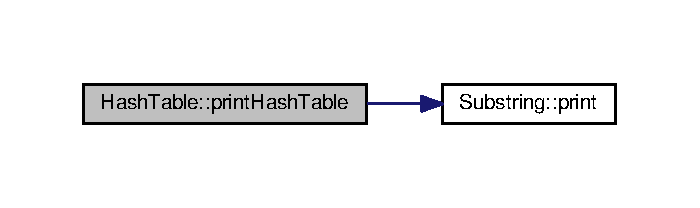
\includegraphics[width=336pt]{classHashTable_a9575e866f5584fadffbcce7b7771c33c_cgraph}
\end{center}
\end{figure}




\subsection{Member Data Documentation}
\hypertarget{classHashTable_ac09c30fbbee3c3a526220ed51074b957}{\index{Hash\+Table@{Hash\+Table}!hash\+Table\+Size@{hash\+Table\+Size}}
\index{hash\+Table\+Size@{hash\+Table\+Size}!Hash\+Table@{Hash\+Table}}
\subsubsection[{hash\+Table\+Size}]{\setlength{\rightskip}{0pt plus 5cm}template$<$typename Type\+Of\+Content$>$ int {\bf Hash\+Table}$<$ Type\+Of\+Content $>$\+::hash\+Table\+Size}}\label{classHashTable_ac09c30fbbee3c3a526220ed51074b957}


quantidade de valores diferentes possiveis para o valor da hash 



Definition at line 43 of file Hash\+Table.\+h.

\hypertarget{classHashTable_a1772210583a06ad2f1039e7fecbc588c}{\index{Hash\+Table@{Hash\+Table}!table@{table}}
\index{table@{table}!Hash\+Table@{Hash\+Table}}
\subsubsection[{table}]{\setlength{\rightskip}{0pt plus 5cm}template$<$typename Type\+Of\+Content$>$ {\bf List\+Of\+Substrings}$<$Type\+Of\+Content$>$$\ast$ {\bf Hash\+Table}$<$ Type\+Of\+Content $>$\+::table}}\label{classHashTable_a1772210583a06ad2f1039e7fecbc588c}


vetor de listas de substrings (uma para cada possivel valor de hash) 



Definition at line 46 of file Hash\+Table.\+h.



Referenced by R\+K\+R\+G\+S\+T$<$ Type\+Of\+Content $>$\+::scan\+Pattern().



The documentation for this class was generated from the following file\+:\begin{DoxyCompactItemize}
\item 
\hyperlink{HashTable_8h}{Hash\+Table.\+h}\end{DoxyCompactItemize}

\hypertarget{classLetter}{\section{Letter$<$ Type\+Of\+Content $>$ Class Template Reference}
\label{classLetter}\index{Letter$<$ Type\+Of\+Content $>$@{Letter$<$ Type\+Of\+Content $>$}}
}


{\ttfamily \#include $<$Letter.\+h$>$}

\subsection*{Public Attributes}
\begin{DoxyCompactItemize}
\item 
int \hyperlink{classLetter_a88ed419ad80a3c9e773f2c2dd0fafe97}{next\+Unmarked}
\begin{DoxyCompactList}\small\item\em Índice da \hyperlink{classLetter}{Letter} não marcada posterior a esta. \end{DoxyCompactList}\item 
int \hyperlink{classLetter_a8b0435db39f7a35dd3874f981d7f19e6}{previous\+Unmarked}
\begin{DoxyCompactList}\small\item\em Índice da \hyperlink{classLetter}{Letter} não marcada anterior a esta. \end{DoxyCompactList}\item 
bool \hyperlink{classLetter_a720835d4e8e538b206ce5cb93da530a8}{marked}
\begin{DoxyCompactList}\small\item\em True caso esta \hyperlink{classLetter}{Letter} está marcada e false caso contrário. \end{DoxyCompactList}\item 
Type\+Of\+Content \hyperlink{classLetter_a9b3d3b6fe677bf9e96a034f71beda5c4}{content}
\begin{DoxyCompactList}\small\item\em Conteúdo da \hyperlink{classLetter}{Letter}. \end{DoxyCompactList}\end{DoxyCompactItemize}


\subsection{Detailed Description}
\subsubsection*{template$<$typename Type\+Of\+Content$>$class Letter$<$ Type\+Of\+Content $>$}


\begin{DoxyTemplParams}{Template Parameters}
{\em Type\+Of\+Content} & tipo da letra do alfabeto utilizado. Tipo dos termos da pattern e da text Classe que armazena cada letra lida do alfabeto em questão \\
\hline
\end{DoxyTemplParams}


Definition at line 29 of file Letter.\+h.



\subsection{Member Data Documentation}
\hypertarget{classLetter_a9b3d3b6fe677bf9e96a034f71beda5c4}{\index{Letter@{Letter}!content@{content}}
\index{content@{content}!Letter@{Letter}}
\subsubsection[{content}]{\setlength{\rightskip}{0pt plus 5cm}template$<$typename Type\+Of\+Content$>$ Type\+Of\+Content {\bf Letter}$<$ Type\+Of\+Content $>$\+::content}}\label{classLetter_a9b3d3b6fe677bf9e96a034f71beda5c4}


Conteúdo da \hyperlink{classLetter}{Letter}. 



Definition at line 45 of file Letter.\+h.

\hypertarget{classLetter_a720835d4e8e538b206ce5cb93da530a8}{\index{Letter@{Letter}!marked@{marked}}
\index{marked@{marked}!Letter@{Letter}}
\subsubsection[{marked}]{\setlength{\rightskip}{0pt plus 5cm}template$<$typename Type\+Of\+Content$>$ bool {\bf Letter}$<$ Type\+Of\+Content $>$\+::marked}}\label{classLetter_a720835d4e8e538b206ce5cb93da530a8}


True caso esta \hyperlink{classLetter}{Letter} está marcada e false caso contrário. 



Definition at line 42 of file Letter.\+h.

\hypertarget{classLetter_a88ed419ad80a3c9e773f2c2dd0fafe97}{\index{Letter@{Letter}!next\+Unmarked@{next\+Unmarked}}
\index{next\+Unmarked@{next\+Unmarked}!Letter@{Letter}}
\subsubsection[{next\+Unmarked}]{\setlength{\rightskip}{0pt plus 5cm}template$<$typename Type\+Of\+Content$>$ int {\bf Letter}$<$ Type\+Of\+Content $>$\+::next\+Unmarked}}\label{classLetter_a88ed419ad80a3c9e773f2c2dd0fafe97}


Índice da \hyperlink{classLetter}{Letter} não marcada posterior a esta. 



Definition at line 37 of file Letter.\+h.

\hypertarget{classLetter_a8b0435db39f7a35dd3874f981d7f19e6}{\index{Letter@{Letter}!previous\+Unmarked@{previous\+Unmarked}}
\index{previous\+Unmarked@{previous\+Unmarked}!Letter@{Letter}}
\subsubsection[{previous\+Unmarked}]{\setlength{\rightskip}{0pt plus 5cm}template$<$typename Type\+Of\+Content$>$ int {\bf Letter}$<$ Type\+Of\+Content $>$\+::previous\+Unmarked}}\label{classLetter_a8b0435db39f7a35dd3874f981d7f19e6}


Índice da \hyperlink{classLetter}{Letter} não marcada anterior a esta. 



Definition at line 39 of file Letter.\+h.



The documentation for this class was generated from the following file\+:\begin{DoxyCompactItemize}
\item 
\hyperlink{Letter_8h}{Letter.\+h}\end{DoxyCompactItemize}

\hypertarget{classListOfMatches}{\section{List\+Of\+Matches Class Reference}
\label{classListOfMatches}\index{List\+Of\+Matches@{List\+Of\+Matches}}
}


{\ttfamily \#include $<$List\+Of\+Matches.\+h$>$}



Collaboration diagram for List\+Of\+Matches\+:\nopagebreak
\begin{figure}[H]
\begin{center}
\leavevmode
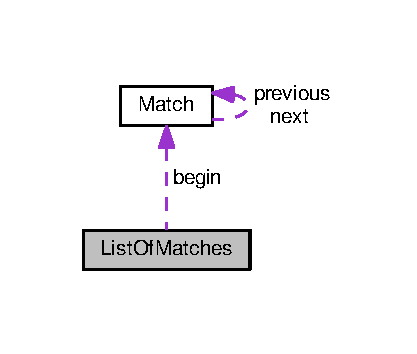
\includegraphics[width=200pt]{classListOfMatches__coll__graph}
\end{center}
\end{figure}
\subsection*{Public Member Functions}
\begin{DoxyCompactItemize}
\item 
\hyperlink{classListOfMatches_a072714a38619e642eda703dfa94fa79c}{List\+Of\+Matches} ()
\item 
void \hyperlink{classListOfMatches_a44472d7bbe64b949bf8ce289bda3134f}{insert} (int length, int pattern\+Index, int text\+Index)
\item 
\hyperlink{classMatch}{Match} $\ast$ \hyperlink{classListOfMatches_a58a6a1649e3731b0e9af20211e4fd03f}{remove} ()
\end{DoxyCompactItemize}
\subsection*{Public Attributes}
\begin{DoxyCompactItemize}
\item 
int \hyperlink{classListOfMatches_ab5b4c972df3758bed3fd5ace4d78a4c8}{number\+Of\+Matches}
\begin{DoxyCompactList}\small\item\em Número de casamentos (objetos da classe \hyperlink{classMatch}{Match}) na lista. \end{DoxyCompactList}\item 
\hyperlink{classMatch}{Match} $\ast$ \hyperlink{classListOfMatches_adc4925222fa338afdbbcdd7e5c37e2c9}{begin}
\begin{DoxyCompactList}\small\item\em Ponteiro para o início da lista. \end{DoxyCompactList}\end{DoxyCompactItemize}


\subsection{Detailed Description}
Lista de casamentos (objetos da classe \hyperlink{classMatch}{Match}) 

Definition at line 33 of file List\+Of\+Matches.\+h.



\subsection{Constructor \& Destructor Documentation}
\hypertarget{classListOfMatches_a072714a38619e642eda703dfa94fa79c}{\index{List\+Of\+Matches@{List\+Of\+Matches}!List\+Of\+Matches@{List\+Of\+Matches}}
\index{List\+Of\+Matches@{List\+Of\+Matches}!List\+Of\+Matches@{List\+Of\+Matches}}
\subsubsection[{List\+Of\+Matches}]{\setlength{\rightskip}{0pt plus 5cm}List\+Of\+Matches\+::\+List\+Of\+Matches (
\begin{DoxyParamCaption}
{}
\end{DoxyParamCaption}
)\hspace{0.3cm}{\ttfamily [inline]}}}\label{classListOfMatches_a072714a38619e642eda703dfa94fa79c}
Construtor de objeto da classe \hyperlink{classListOfMatches}{List\+Of\+Matches} 

Definition at line 43 of file List\+Of\+Matches.\+h.



\subsection{Member Function Documentation}
\hypertarget{classListOfMatches_a44472d7bbe64b949bf8ce289bda3134f}{\index{List\+Of\+Matches@{List\+Of\+Matches}!insert@{insert}}
\index{insert@{insert}!List\+Of\+Matches@{List\+Of\+Matches}}
\subsubsection[{insert}]{\setlength{\rightskip}{0pt plus 5cm}void List\+Of\+Matches\+::insert (
\begin{DoxyParamCaption}
\item[{int}]{length, }
\item[{int}]{pattern\+Index, }
\item[{int}]{text\+Index}
\end{DoxyParamCaption}
)}}\label{classListOfMatches_a44472d7bbe64b949bf8ce289bda3134f}
Insere casamento (objeto da classe \hyperlink{classMatch}{Match}) 
\begin{DoxyParams}{Parameters}
{\em length} & Tamanho do casamento (objeto da classe \hyperlink{classMatch}{Match}) a ser inserido. \\
\hline
{\em pattern\+Index} & Índice em pattern do casamento (objeto da classe \hyperlink{classMatch}{Match}) a ser inserido. \\
\hline
{\em text\+Index} & Índice em text do casamento (objeto da classe \hyperlink{classMatch}{Match}) a ser inserido. \\
\hline
\end{DoxyParams}


Definition at line 26 of file List\+Of\+Matches.\+cpp.



References begin, Match\+::length, Match\+::next, number\+Of\+Matches, and Match\+::previous.



Referenced by R\+K\+R\+G\+S\+T$<$ Type\+Of\+Content $>$\+::mark\+Arrays(), and R\+K\+R\+G\+S\+T$<$ Type\+Of\+Content $>$\+::scan\+Pattern().

\hypertarget{classListOfMatches_a58a6a1649e3731b0e9af20211e4fd03f}{\index{List\+Of\+Matches@{List\+Of\+Matches}!remove@{remove}}
\index{remove@{remove}!List\+Of\+Matches@{List\+Of\+Matches}}
\subsubsection[{remove}]{\setlength{\rightskip}{0pt plus 5cm}{\bf Match} $\ast$ List\+Of\+Matches\+::remove (
\begin{DoxyParamCaption}
{}
\end{DoxyParamCaption}
)}}\label{classListOfMatches_a58a6a1649e3731b0e9af20211e4fd03f}
Remove um match da lista 

Definition at line 78 of file List\+Of\+Matches.\+cpp.



References begin, Match\+::next, number\+Of\+Matches, and Match\+::previous.



Referenced by main(), and R\+K\+R\+G\+S\+T$<$ Type\+Of\+Content $>$\+::mark\+Arrays().



\subsection{Member Data Documentation}
\hypertarget{classListOfMatches_adc4925222fa338afdbbcdd7e5c37e2c9}{\index{List\+Of\+Matches@{List\+Of\+Matches}!begin@{begin}}
\index{begin@{begin}!List\+Of\+Matches@{List\+Of\+Matches}}
\subsubsection[{begin}]{\setlength{\rightskip}{0pt plus 5cm}{\bf Match}$\ast$ List\+Of\+Matches\+::begin}}\label{classListOfMatches_adc4925222fa338afdbbcdd7e5c37e2c9}


Ponteiro para o início da lista. 



Definition at line 39 of file List\+Of\+Matches.\+h.



Referenced by insert(), and remove().

\hypertarget{classListOfMatches_ab5b4c972df3758bed3fd5ace4d78a4c8}{\index{List\+Of\+Matches@{List\+Of\+Matches}!number\+Of\+Matches@{number\+Of\+Matches}}
\index{number\+Of\+Matches@{number\+Of\+Matches}!List\+Of\+Matches@{List\+Of\+Matches}}
\subsubsection[{number\+Of\+Matches}]{\setlength{\rightskip}{0pt plus 5cm}int List\+Of\+Matches\+::number\+Of\+Matches}}\label{classListOfMatches_ab5b4c972df3758bed3fd5ace4d78a4c8}


Número de casamentos (objetos da classe \hyperlink{classMatch}{Match}) na lista. 



Definition at line 37 of file List\+Of\+Matches.\+h.



Referenced by insert(), main(), R\+K\+R\+G\+S\+T$<$ Type\+Of\+Content $>$\+::mark\+Arrays(), and remove().



The documentation for this class was generated from the following files\+:\begin{DoxyCompactItemize}
\item 
\hyperlink{ListOfMatches_8h}{List\+Of\+Matches.\+h}\item 
\hyperlink{ListOfMatches_8cpp}{List\+Of\+Matches.\+cpp}\end{DoxyCompactItemize}

\hypertarget{classListOfSubstrings}{\section{List\+Of\+Substrings$<$ Type\+Of\+Content $>$ Class Template Reference}
\label{classListOfSubstrings}\index{List\+Of\+Substrings$<$ Type\+Of\+Content $>$@{List\+Of\+Substrings$<$ Type\+Of\+Content $>$}}
}


{\ttfamily \#include $<$List\+Of\+Substrings.\+h$>$}

\subsection*{Public Member Functions}
\begin{DoxyCompactItemize}
\item 
\hyperlink{classListOfSubstrings_ab8280100b0f6224eb4d36fc448d8eeb8}{List\+Of\+Substrings} ()
\begin{DoxyCompactList}\small\item\em Construtor de \hyperlink{classListOfSubstrings}{List\+Of\+Substrings}. \end{DoxyCompactList}\item 
\hyperlink{classListOfSubstrings_ae5aa0c336f8f5fab58a8d239cc5ab9d9}{$\sim$\+List\+Of\+Substrings} ()
\item 
void \hyperlink{classListOfSubstrings_a480372956993999a6e42e104cf264e32}{add\+Substring} (\hyperlink{classSubstring}{Substring}$<$ Type\+Of\+Content $>$ $\ast$substring)
\end{DoxyCompactItemize}
\subsection*{Public Attributes}
\begin{DoxyCompactItemize}
\item 
int \hyperlink{classListOfSubstrings_afbd8ea432d107cd2f1285c9fe5dd9b96}{number\+Of\+Substrings}
\begin{DoxyCompactList}\small\item\em Número de objetos da classe \hyperlink{classSubstring}{Substring} na lista. \end{DoxyCompactList}\item 
\hyperlink{classSubstring}{Substring}$<$ Type\+Of\+Content $>$ $\ast$ \hyperlink{classListOfSubstrings_aca3c37e86411bf80050bece7a1ec0df0}{begin}
\begin{DoxyCompactList}\small\item\em Ponteiro para o início da lista. \end{DoxyCompactList}\item 
\hyperlink{classSubstring}{Substring}$<$ Type\+Of\+Content $>$ $\ast$ \hyperlink{classListOfSubstrings_a4b4c8edcbdf74d6c6b0e21551e504b98}{end}
\begin{DoxyCompactList}\small\item\em Ponteiro para o fim da lista. \end{DoxyCompactList}\end{DoxyCompactItemize}


\subsection{Detailed Description}
\subsubsection*{template$<$typename Type\+Of\+Content$>$class List\+Of\+Substrings$<$ Type\+Of\+Content $>$}

Lista de objetos da classe \hyperlink{classSubstring}{Substring} 
\begin{DoxyTemplParams}{Template Parameters}
{\em Type\+Of\+Content} & tipo da letra do alfabeto utilizado. Tipo dos termos da pattern e da text \\
\hline
\end{DoxyTemplParams}
\begin{DoxySeeAlso}{See also}
\hyperlink{classSubstring}{Substring} 
\end{DoxySeeAlso}


Definition at line 34 of file List\+Of\+Substrings.\+h.



\subsection{Constructor \& Destructor Documentation}
\hypertarget{classListOfSubstrings_ab8280100b0f6224eb4d36fc448d8eeb8}{\index{List\+Of\+Substrings@{List\+Of\+Substrings}!List\+Of\+Substrings@{List\+Of\+Substrings}}
\index{List\+Of\+Substrings@{List\+Of\+Substrings}!List\+Of\+Substrings@{List\+Of\+Substrings}}
\subsubsection[{List\+Of\+Substrings}]{\setlength{\rightskip}{0pt plus 5cm}template$<$typename Type\+Of\+Content$>$ {\bf List\+Of\+Substrings}$<$ Type\+Of\+Content $>$\+::{\bf List\+Of\+Substrings} (
\begin{DoxyParamCaption}
{}
\end{DoxyParamCaption}
)\hspace{0.3cm}{\ttfamily [inline]}}}\label{classListOfSubstrings_ab8280100b0f6224eb4d36fc448d8eeb8}


Construtor de \hyperlink{classListOfSubstrings}{List\+Of\+Substrings}. 



Definition at line 48 of file List\+Of\+Substrings.\+h.

\hypertarget{classListOfSubstrings_ae5aa0c336f8f5fab58a8d239cc5ab9d9}{\index{List\+Of\+Substrings@{List\+Of\+Substrings}!````~List\+Of\+Substrings@{$\sim$\+List\+Of\+Substrings}}
\index{````~List\+Of\+Substrings@{$\sim$\+List\+Of\+Substrings}!List\+Of\+Substrings@{List\+Of\+Substrings}}
\subsubsection[{$\sim$\+List\+Of\+Substrings}]{\setlength{\rightskip}{0pt plus 5cm}template$<$typename Type\+Of\+Content$>$ {\bf List\+Of\+Substrings}$<$ Type\+Of\+Content $>$\+::$\sim${\bf List\+Of\+Substrings} (
\begin{DoxyParamCaption}
{}
\end{DoxyParamCaption}
)\hspace{0.3cm}{\ttfamily [inline]}}}\label{classListOfSubstrings_ae5aa0c336f8f5fab58a8d239cc5ab9d9}
Destrutor de \hyperlink{classListOfSubstrings}{List\+Of\+Substrings}. deletando cada um dos objetos da classe Substrings contidos na lista 

Definition at line 60 of file List\+Of\+Substrings.\+h.



References Substring$<$ Type\+Of\+Content $>$\+::next.



\subsection{Member Function Documentation}
\hypertarget{classListOfSubstrings_a480372956993999a6e42e104cf264e32}{\index{List\+Of\+Substrings@{List\+Of\+Substrings}!add\+Substring@{add\+Substring}}
\index{add\+Substring@{add\+Substring}!List\+Of\+Substrings@{List\+Of\+Substrings}}
\subsubsection[{add\+Substring}]{\setlength{\rightskip}{0pt plus 5cm}template$<$typename Type\+Of\+Content$>$ void {\bf List\+Of\+Substrings}$<$ Type\+Of\+Content $>$\+::add\+Substring (
\begin{DoxyParamCaption}
\item[{{\bf Substring}$<$ Type\+Of\+Content $>$ $\ast$}]{substring}
\end{DoxyParamCaption}
)\hspace{0.3cm}{\ttfamily [inline]}}}\label{classListOfSubstrings_a480372956993999a6e42e104cf264e32}
Adiciona uma nova substring a lista de substrings 
\begin{DoxyParams}{Parameters}
{\em substring} & substring que será adicionada. \\
\hline
\end{DoxyParams}


Definition at line 78 of file List\+Of\+Substrings.\+h.



References List\+Of\+Substrings$<$ Type\+Of\+Content $>$\+::end, Substring$<$ Type\+Of\+Content $>$\+::next, and Substring$<$ Type\+Of\+Content $>$\+::previous.



\subsection{Member Data Documentation}
\hypertarget{classListOfSubstrings_aca3c37e86411bf80050bece7a1ec0df0}{\index{List\+Of\+Substrings@{List\+Of\+Substrings}!begin@{begin}}
\index{begin@{begin}!List\+Of\+Substrings@{List\+Of\+Substrings}}
\subsubsection[{begin}]{\setlength{\rightskip}{0pt plus 5cm}template$<$typename Type\+Of\+Content$>$ {\bf Substring}$<$Type\+Of\+Content$>$$\ast$ {\bf List\+Of\+Substrings}$<$ Type\+Of\+Content $>$\+::begin}}\label{classListOfSubstrings_aca3c37e86411bf80050bece7a1ec0df0}


Ponteiro para o início da lista. 



Definition at line 42 of file List\+Of\+Substrings.\+h.

\hypertarget{classListOfSubstrings_a4b4c8edcbdf74d6c6b0e21551e504b98}{\index{List\+Of\+Substrings@{List\+Of\+Substrings}!end@{end}}
\index{end@{end}!List\+Of\+Substrings@{List\+Of\+Substrings}}
\subsubsection[{end}]{\setlength{\rightskip}{0pt plus 5cm}template$<$typename Type\+Of\+Content$>$ {\bf Substring}$<$Type\+Of\+Content$>$$\ast$ {\bf List\+Of\+Substrings}$<$ Type\+Of\+Content $>$\+::end}}\label{classListOfSubstrings_a4b4c8edcbdf74d6c6b0e21551e504b98}


Ponteiro para o fim da lista. 



Definition at line 45 of file List\+Of\+Substrings.\+h.



Referenced by List\+Of\+Substrings$<$ Type\+Of\+Content $>$\+::add\+Substring().

\hypertarget{classListOfSubstrings_afbd8ea432d107cd2f1285c9fe5dd9b96}{\index{List\+Of\+Substrings@{List\+Of\+Substrings}!number\+Of\+Substrings@{number\+Of\+Substrings}}
\index{number\+Of\+Substrings@{number\+Of\+Substrings}!List\+Of\+Substrings@{List\+Of\+Substrings}}
\subsubsection[{number\+Of\+Substrings}]{\setlength{\rightskip}{0pt plus 5cm}template$<$typename Type\+Of\+Content$>$ int {\bf List\+Of\+Substrings}$<$ Type\+Of\+Content $>$\+::number\+Of\+Substrings}}\label{classListOfSubstrings_afbd8ea432d107cd2f1285c9fe5dd9b96}


Número de objetos da classe \hyperlink{classSubstring}{Substring} na lista. 



Definition at line 39 of file List\+Of\+Substrings.\+h.



The documentation for this class was generated from the following file\+:\begin{DoxyCompactItemize}
\item 
\hyperlink{ListOfSubstrings_8h}{List\+Of\+Substrings.\+h}\end{DoxyCompactItemize}

\hypertarget{classListOfTiles}{\section{List\+Of\+Tiles Class Reference}
\label{classListOfTiles}\index{List\+Of\+Tiles@{List\+Of\+Tiles}}
}


{\ttfamily \#include $<$List\+Of\+Tiles.\+h$>$}



Collaboration diagram for List\+Of\+Tiles\+:\nopagebreak
\begin{figure}[H]
\begin{center}
\leavevmode
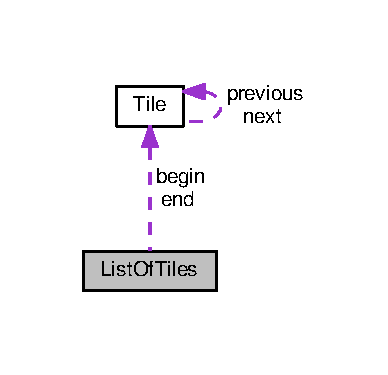
\includegraphics[width=186pt]{classListOfTiles__coll__graph}
\end{center}
\end{figure}
\subsection*{Public Member Functions}
\begin{DoxyCompactItemize}
\item 
\hyperlink{classListOfTiles_ad87132d4a7c3eb474797f3e3be24232c}{List\+Of\+Tiles} ()
\item 
\hyperlink{classListOfTiles_aff2ecd909d48a815199b949f0a0556cc}{$\sim$\+List\+Of\+Tiles} ()
\item 
void \hyperlink{classListOfTiles_a0d8226cb5174084dd6bc7d8854c1e3aa}{add\+Tile} (\hyperlink{classTile}{Tile} $\ast$tile)
\item 
void \hyperlink{classListOfTiles_a72a1b46b241ee17dc6f6ff9e5f291521}{print} ()
\item 
void \hyperlink{classListOfTiles_ac824d0c735f0f975663740da8d827511}{remove\+Tile} (int tile\+Begin\+Index, int tile\+End\+Index)
\end{DoxyCompactItemize}
\subsection*{Public Attributes}
\begin{DoxyCompactItemize}
\item 
\hyperlink{classTile}{Tile} $\ast$ \hyperlink{classListOfTiles_a19f2f2aac9802594a1080a199fa5b3b7}{begin}
\begin{DoxyCompactList}\small\item\em Ponteiro para o primeiro objeto do tipo \hyperlink{classTile}{Tile} na lista. \end{DoxyCompactList}\item 
\hyperlink{classTile}{Tile} $\ast$ \hyperlink{classListOfTiles_adebd46c83a63f0e0f385cc0170def3b3}{end}
\begin{DoxyCompactList}\small\item\em Ponteiro para o último objeto do tipo \hyperlink{classTile}{Tile} na lista. \end{DoxyCompactList}\item 
int \hyperlink{classListOfTiles_a6d6a5a454a10f1a9ea1fd4bc4dedf290}{number\+Of\+Tiles}
\begin{DoxyCompactList}\small\item\em Quantidade de objetos do tipo \hyperlink{classTile}{Tile} na lista. \end{DoxyCompactList}\end{DoxyCompactItemize}


\subsection{Detailed Description}
Classe que guarda objetos do tipo \hyperlink{classTile}{Tile} \begin{DoxySeeAlso}{See also}
\hyperlink{classTile}{Tile} 
\end{DoxySeeAlso}


Definition at line 39 of file List\+Of\+Tiles.\+h.



\subsection{Constructor \& Destructor Documentation}
\hypertarget{classListOfTiles_ad87132d4a7c3eb474797f3e3be24232c}{\index{List\+Of\+Tiles@{List\+Of\+Tiles}!List\+Of\+Tiles@{List\+Of\+Tiles}}
\index{List\+Of\+Tiles@{List\+Of\+Tiles}!List\+Of\+Tiles@{List\+Of\+Tiles}}
\subsubsection[{List\+Of\+Tiles}]{\setlength{\rightskip}{0pt plus 5cm}List\+Of\+Tiles\+::\+List\+Of\+Tiles (
\begin{DoxyParamCaption}
{}
\end{DoxyParamCaption}
)\hspace{0.3cm}{\ttfamily [inline]}}}\label{classListOfTiles_ad87132d4a7c3eb474797f3e3be24232c}
Construtor de um objeto da classe \hyperlink{classListOfTiles}{List\+Of\+Tiles} 

Definition at line 56 of file List\+Of\+Tiles.\+h.

\hypertarget{classListOfTiles_aff2ecd909d48a815199b949f0a0556cc}{\index{List\+Of\+Tiles@{List\+Of\+Tiles}!````~List\+Of\+Tiles@{$\sim$\+List\+Of\+Tiles}}
\index{````~List\+Of\+Tiles@{$\sim$\+List\+Of\+Tiles}!List\+Of\+Tiles@{List\+Of\+Tiles}}
\subsubsection[{$\sim$\+List\+Of\+Tiles}]{\setlength{\rightskip}{0pt plus 5cm}List\+Of\+Tiles\+::$\sim$\+List\+Of\+Tiles (
\begin{DoxyParamCaption}
{}
\end{DoxyParamCaption}
)\hspace{0.3cm}{\ttfamily [inline]}}}\label{classListOfTiles_aff2ecd909d48a815199b949f0a0556cc}
Destrutor de um objeto da classe \hyperlink{classListOfTiles}{List\+Of\+Tiles} 

Definition at line 66 of file List\+Of\+Tiles.\+h.



References begin, and Tile\+::next.



\subsection{Member Function Documentation}
\hypertarget{classListOfTiles_a0d8226cb5174084dd6bc7d8854c1e3aa}{\index{List\+Of\+Tiles@{List\+Of\+Tiles}!add\+Tile@{add\+Tile}}
\index{add\+Tile@{add\+Tile}!List\+Of\+Tiles@{List\+Of\+Tiles}}
\subsubsection[{add\+Tile}]{\setlength{\rightskip}{0pt plus 5cm}void List\+Of\+Tiles\+::add\+Tile (
\begin{DoxyParamCaption}
\item[{{\bf Tile} $\ast$}]{tile}
\end{DoxyParamCaption}
)\hspace{0.3cm}{\ttfamily [inline]}}}\label{classListOfTiles_a0d8226cb5174084dd6bc7d8854c1e3aa}
Adiciona um novo objeto da classe \hyperlink{classTile}{Tile} na lista 
\begin{DoxyParams}{Parameters}
{\em tile} & Ponteiro para o objeto da classe \hyperlink{classTile}{Tile} a ser adicionado \\
\hline
\end{DoxyParams}
\begin{DoxyReturn}{Returns}
Não há retorno 
\end{DoxyReturn}


Definition at line 89 of file List\+Of\+Tiles.\+h.



References end, Tile\+::next, and Tile\+::previous.

\hypertarget{classListOfTiles_a72a1b46b241ee17dc6f6ff9e5f291521}{\index{List\+Of\+Tiles@{List\+Of\+Tiles}!print@{print}}
\index{print@{print}!List\+Of\+Tiles@{List\+Of\+Tiles}}
\subsubsection[{print}]{\setlength{\rightskip}{0pt plus 5cm}void List\+Of\+Tiles\+::print (
\begin{DoxyParamCaption}
{}
\end{DoxyParamCaption}
)\hspace{0.3cm}{\ttfamily [inline]}}}\label{classListOfTiles_a72a1b46b241ee17dc6f6ff9e5f291521}
Imprime, para cada objeto da classe \hyperlink{classTile}{Tile} na lista, o seu índice de início e de fim. \begin{DoxyReturn}{Returns}
Não há retorno 
\end{DoxyReturn}


Definition at line 113 of file List\+Of\+Tiles.\+h.



References Tile\+::begin, begin, Tile\+::end, and Tile\+::next.

\hypertarget{classListOfTiles_ac824d0c735f0f975663740da8d827511}{\index{List\+Of\+Tiles@{List\+Of\+Tiles}!remove\+Tile@{remove\+Tile}}
\index{remove\+Tile@{remove\+Tile}!List\+Of\+Tiles@{List\+Of\+Tiles}}
\subsubsection[{remove\+Tile}]{\setlength{\rightskip}{0pt plus 5cm}void List\+Of\+Tiles\+::remove\+Tile (
\begin{DoxyParamCaption}
\item[{int}]{tile\+Begin\+Index, }
\item[{int}]{tile\+End\+Index}
\end{DoxyParamCaption}
)\hspace{0.3cm}{\ttfamily [inline]}}}\label{classListOfTiles_ac824d0c735f0f975663740da8d827511}
Remove objeto da classe \hyperlink{classTile}{Tile} 
\begin{DoxyParams}{Parameters}
{\em tile\+Begin\+Index} & Índice da primeira posição da tile a ser removida \\
\hline
{\em tile\+End\+Index} & Índice da última posição da tile a ser removida \\
\hline
\end{DoxyParams}
\begin{DoxyReturn}{Returns}
Não há retorno 
\end{DoxyReturn}


Definition at line 130 of file List\+Of\+Tiles.\+h.



References Tile\+::begin, begin, Tile\+::end, Tile\+::next, and Tile\+::previous.



\subsection{Member Data Documentation}
\hypertarget{classListOfTiles_a19f2f2aac9802594a1080a199fa5b3b7}{\index{List\+Of\+Tiles@{List\+Of\+Tiles}!begin@{begin}}
\index{begin@{begin}!List\+Of\+Tiles@{List\+Of\+Tiles}}
\subsubsection[{begin}]{\setlength{\rightskip}{0pt plus 5cm}{\bf Tile}$\ast$ List\+Of\+Tiles\+::begin}}\label{classListOfTiles_a19f2f2aac9802594a1080a199fa5b3b7}


Ponteiro para o primeiro objeto do tipo \hyperlink{classTile}{Tile} na lista. 



Definition at line 45 of file List\+Of\+Tiles.\+h.



Referenced by R\+K\+R\+G\+S\+T$<$ Type\+Of\+Content $>$\+::fill\+Text\+Hash\+Table(), R\+K\+R\+G\+S\+T$<$ Type\+Of\+Content $>$\+::find\+Pattern\+Substring(), print(), remove\+Tile(), and $\sim$\+List\+Of\+Tiles().

\hypertarget{classListOfTiles_adebd46c83a63f0e0f385cc0170def3b3}{\index{List\+Of\+Tiles@{List\+Of\+Tiles}!end@{end}}
\index{end@{end}!List\+Of\+Tiles@{List\+Of\+Tiles}}
\subsubsection[{end}]{\setlength{\rightskip}{0pt plus 5cm}{\bf Tile}$\ast$ List\+Of\+Tiles\+::end}}\label{classListOfTiles_adebd46c83a63f0e0f385cc0170def3b3}


Ponteiro para o último objeto do tipo \hyperlink{classTile}{Tile} na lista. 



Definition at line 48 of file List\+Of\+Tiles.\+h.



Referenced by add\+Tile().

\hypertarget{classListOfTiles_a6d6a5a454a10f1a9ea1fd4bc4dedf290}{\index{List\+Of\+Tiles@{List\+Of\+Tiles}!number\+Of\+Tiles@{number\+Of\+Tiles}}
\index{number\+Of\+Tiles@{number\+Of\+Tiles}!List\+Of\+Tiles@{List\+Of\+Tiles}}
\subsubsection[{number\+Of\+Tiles}]{\setlength{\rightskip}{0pt plus 5cm}int List\+Of\+Tiles\+::number\+Of\+Tiles}}\label{classListOfTiles_a6d6a5a454a10f1a9ea1fd4bc4dedf290}


Quantidade de objetos do tipo \hyperlink{classTile}{Tile} na lista. 



Definition at line 51 of file List\+Of\+Tiles.\+h.



The documentation for this class was generated from the following file\+:\begin{DoxyCompactItemize}
\item 
\hyperlink{ListOfTiles_8h}{List\+Of\+Tiles.\+h}\end{DoxyCompactItemize}

\hypertarget{classMatch}{\section{Match Class Reference}
\label{classMatch}\index{Match@{Match}}
}


{\ttfamily \#include $<$Match.\+h$>$}



Collaboration diagram for Match\+:\nopagebreak
\begin{figure}[H]
\begin{center}
\leavevmode
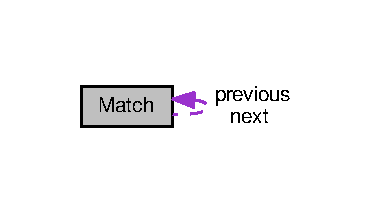
\includegraphics[width=181pt]{classMatch__coll__graph}
\end{center}
\end{figure}
\subsection*{Public Member Functions}
\begin{DoxyCompactItemize}
\item 
\hyperlink{classMatch_a05b81a2405d43e106a8b2488a4108c56}{Match} (int \hyperlink{classMatch_aa7e6b74eb7831de7a921ef7d3655d19a}{length}, int \hyperlink{classMatch_ac673bad1075e5499f0d857ed0a526fa2}{pattern\+Index}, int \hyperlink{classMatch_aee534a2e3d23f7d069a618e1cb7b6343}{text\+Index})
\item 
void \hyperlink{classMatch_a4f14830202018dc00166f78572c11c8f}{print} ()
\end{DoxyCompactItemize}
\subsection*{Public Attributes}
\begin{DoxyCompactItemize}
\item 
int \hyperlink{classMatch_aa7e6b74eb7831de7a921ef7d3655d19a}{length}
\begin{DoxyCompactList}\small\item\em tamanho do casamento \end{DoxyCompactList}\item 
int \hyperlink{classMatch_ac673bad1075e5499f0d857ed0a526fa2}{pattern\+Index}
\begin{DoxyCompactList}\small\item\em indice em pattern da primeira letra pertencente ao casamento \end{DoxyCompactList}\item 
int \hyperlink{classMatch_aee534a2e3d23f7d069a618e1cb7b6343}{text\+Index}
\begin{DoxyCompactList}\small\item\em indice em text da primeira letra pertencente ao casamento \end{DoxyCompactList}\item 
\hyperlink{classMatch}{Match} $\ast$ \hyperlink{classMatch_a992c150265becb5f6806d09bad8cea0c}{next}
\begin{DoxyCompactList}\small\item\em Ponteiro para o proximo casamento em uma estrutura que engloba um objeto desta classe. \end{DoxyCompactList}\item 
\hyperlink{classMatch}{Match} $\ast$ \hyperlink{classMatch_aec1e648b8eba83f2ed76182644ce91de}{previous}
\begin{DoxyCompactList}\small\item\em Ponteiro para o casamento anterior em uma estrutura que engloba um objeto desta classe. \end{DoxyCompactList}\end{DoxyCompactItemize}


\subsection{Detailed Description}
Classe que representa um casamento. 

Definition at line 29 of file Match.\+h.



\subsection{Constructor \& Destructor Documentation}
\hypertarget{classMatch_a05b81a2405d43e106a8b2488a4108c56}{\index{Match@{Match}!Match@{Match}}
\index{Match@{Match}!Match@{Match}}
\subsubsection[{Match}]{\setlength{\rightskip}{0pt plus 5cm}Match\+::\+Match (
\begin{DoxyParamCaption}
\item[{int}]{length, }
\item[{int}]{pattern\+Index, }
\item[{int}]{text\+Index}
\end{DoxyParamCaption}
)\hspace{0.3cm}{\ttfamily [inline]}}}\label{classMatch_a05b81a2405d43e106a8b2488a4108c56}
Construtor de um objeto da classe \hyperlink{classMatch}{Match} 
\begin{DoxyParams}{Parameters}
{\em length} & Tamanho do casamento. \\
\hline
{\em pattern\+Index} & Indice em pattern da primeira letra pertencente ao casamento. \\
\hline
{\em text\+Index} & Indice em pattern da primeira letra pertencente ao casamento. \\
\hline
\end{DoxyParams}


Definition at line 50 of file Match.\+h.



\subsection{Member Function Documentation}
\hypertarget{classMatch_a4f14830202018dc00166f78572c11c8f}{\index{Match@{Match}!print@{print}}
\index{print@{print}!Match@{Match}}
\subsubsection[{print}]{\setlength{\rightskip}{0pt plus 5cm}void Match\+::print (
\begin{DoxyParamCaption}
{}
\end{DoxyParamCaption}
)\hspace{0.3cm}{\ttfamily [inline]}}}\label{classMatch_a4f14830202018dc00166f78572c11c8f}
Método que imprime o conteúdo do objeto da classe \hyperlink{classMatch}{Match}. 

Definition at line 61 of file Match.\+h.



Referenced by main().



\subsection{Member Data Documentation}
\hypertarget{classMatch_aa7e6b74eb7831de7a921ef7d3655d19a}{\index{Match@{Match}!length@{length}}
\index{length@{length}!Match@{Match}}
\subsubsection[{length}]{\setlength{\rightskip}{0pt plus 5cm}int Match\+::length}}\label{classMatch_aa7e6b74eb7831de7a921ef7d3655d19a}


tamanho do casamento 



Definition at line 33 of file Match.\+h.



Referenced by List\+Of\+Matches\+::insert(), main(), R\+K\+R\+G\+S\+T$<$ Type\+Of\+Content $>$\+::mark\+Arrays(), R\+K\+R\+G\+S\+T$<$ Type\+Of\+Content $>$\+::mark\+Tokens(), and R\+K\+R\+G\+S\+T$<$ Type\+Of\+Content $>$\+::occluded().

\hypertarget{classMatch_a992c150265becb5f6806d09bad8cea0c}{\index{Match@{Match}!next@{next}}
\index{next@{next}!Match@{Match}}
\subsubsection[{next}]{\setlength{\rightskip}{0pt plus 5cm}{\bf Match}$\ast$ Match\+::next}}\label{classMatch_a992c150265becb5f6806d09bad8cea0c}


Ponteiro para o proximo casamento em uma estrutura que engloba um objeto desta classe. 



Definition at line 40 of file Match.\+h.



Referenced by List\+Of\+Matches\+::insert(), and List\+Of\+Matches\+::remove().

\hypertarget{classMatch_ac673bad1075e5499f0d857ed0a526fa2}{\index{Match@{Match}!pattern\+Index@{pattern\+Index}}
\index{pattern\+Index@{pattern\+Index}!Match@{Match}}
\subsubsection[{pattern\+Index}]{\setlength{\rightskip}{0pt plus 5cm}int Match\+::pattern\+Index}}\label{classMatch_ac673bad1075e5499f0d857ed0a526fa2}


indice em pattern da primeira letra pertencente ao casamento 



Definition at line 35 of file Match.\+h.



Referenced by main(), R\+K\+R\+G\+S\+T$<$ Type\+Of\+Content $>$\+::mark\+Arrays(), R\+K\+R\+G\+S\+T$<$ Type\+Of\+Content $>$\+::mark\+Tokens(), and R\+K\+R\+G\+S\+T$<$ Type\+Of\+Content $>$\+::occluded().

\hypertarget{classMatch_aec1e648b8eba83f2ed76182644ce91de}{\index{Match@{Match}!previous@{previous}}
\index{previous@{previous}!Match@{Match}}
\subsubsection[{previous}]{\setlength{\rightskip}{0pt plus 5cm}{\bf Match}$\ast$ Match\+::previous}}\label{classMatch_aec1e648b8eba83f2ed76182644ce91de}


Ponteiro para o casamento anterior em uma estrutura que engloba um objeto desta classe. 



Definition at line 42 of file Match.\+h.



Referenced by List\+Of\+Matches\+::insert(), and List\+Of\+Matches\+::remove().

\hypertarget{classMatch_aee534a2e3d23f7d069a618e1cb7b6343}{\index{Match@{Match}!text\+Index@{text\+Index}}
\index{text\+Index@{text\+Index}!Match@{Match}}
\subsubsection[{text\+Index}]{\setlength{\rightskip}{0pt plus 5cm}int Match\+::text\+Index}}\label{classMatch_aee534a2e3d23f7d069a618e1cb7b6343}


indice em text da primeira letra pertencente ao casamento 



Definition at line 37 of file Match.\+h.



Referenced by main(), R\+K\+R\+G\+S\+T$<$ Type\+Of\+Content $>$\+::mark\+Arrays(), R\+K\+R\+G\+S\+T$<$ Type\+Of\+Content $>$\+::mark\+Tokens(), and R\+K\+R\+G\+S\+T$<$ Type\+Of\+Content $>$\+::occluded().



The documentation for this class was generated from the following file\+:\begin{DoxyCompactItemize}
\item 
\hyperlink{Match_8h}{Match.\+h}\end{DoxyCompactItemize}

\hypertarget{classRandomNumber}{\section{Random\+Number Class Reference}
\label{classRandomNumber}\index{Random\+Number@{Random\+Number}}
}


{\ttfamily \#include $<$Random\+Number.\+h$>$}

\subsection*{Public Member Functions}
\begin{DoxyCompactItemize}
\item 
\hyperlink{classRandomNumber_a70176ac091c4e563d19658432b504fb3}{Random\+Number} ()
\begin{DoxyCompactList}\small\item\em Construtor que inicializa a semente da função que gera o número aleatório. \end{DoxyCompactList}\item 
int \hyperlink{classRandomNumber_ada5063d81ac44b99407ae29cc2faec6e}{new\+Random\+Number} (int min, int max)
\end{DoxyCompactItemize}


\subsection{Detailed Description}
Cria um número inteiro aleatório entre dois inteiros,min e max. 

Definition at line 30 of file Random\+Number.\+h.



\subsection{Constructor \& Destructor Documentation}
\hypertarget{classRandomNumber_a70176ac091c4e563d19658432b504fb3}{\index{Random\+Number@{Random\+Number}!Random\+Number@{Random\+Number}}
\index{Random\+Number@{Random\+Number}!Random\+Number@{Random\+Number}}
\subsubsection[{Random\+Number}]{\setlength{\rightskip}{0pt plus 5cm}Random\+Number\+::\+Random\+Number (
\begin{DoxyParamCaption}
{}
\end{DoxyParamCaption}
)\hspace{0.3cm}{\ttfamily [inline]}}}\label{classRandomNumber_a70176ac091c4e563d19658432b504fb3}


Construtor que inicializa a semente da função que gera o número aleatório. 



Definition at line 34 of file Random\+Number.\+h.



\subsection{Member Function Documentation}
\hypertarget{classRandomNumber_ada5063d81ac44b99407ae29cc2faec6e}{\index{Random\+Number@{Random\+Number}!new\+Random\+Number@{new\+Random\+Number}}
\index{new\+Random\+Number@{new\+Random\+Number}!Random\+Number@{Random\+Number}}
\subsubsection[{new\+Random\+Number}]{\setlength{\rightskip}{0pt plus 5cm}int Random\+Number\+::new\+Random\+Number (
\begin{DoxyParamCaption}
\item[{int}]{min, }
\item[{int}]{max}
\end{DoxyParamCaption}
)\hspace{0.3cm}{\ttfamily [inline]}}}\label{classRandomNumber_ada5063d81ac44b99407ae29cc2faec6e}
Gera um número aleatório x, sendo min $<$= x $<$= max 
\begin{DoxyParams}{Parameters}
{\em min} & Valor mínimo possível de ser atribuído ao número criado \\
\hline
{\em max} & Valor máximo possível de ser atribuído ao número criado \\
\hline
\end{DoxyParams}


Definition at line 44 of file Random\+Number.\+h.



Referenced by Random\+Prime\+::new\+Random\+Prime().



The documentation for this class was generated from the following file\+:\begin{DoxyCompactItemize}
\item 
\hyperlink{RandomNumber_8h}{Random\+Number.\+h}\end{DoxyCompactItemize}

\hypertarget{classRandomPrime}{\section{Random\+Prime Class Reference}
\label{classRandomPrime}\index{Random\+Prime@{Random\+Prime}}
}


{\ttfamily \#include $<$Random\+Prime.\+h$>$}



Collaboration diagram for Random\+Prime\+:\nopagebreak
\begin{figure}[H]
\begin{center}
\leavevmode
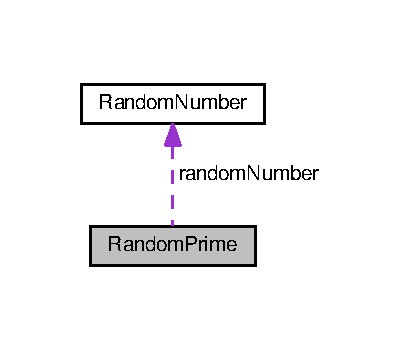
\includegraphics[width=193pt]{classRandomPrime__coll__graph}
\end{center}
\end{figure}
\subsection*{Public Member Functions}
\begin{DoxyCompactItemize}
\item 
\hyperlink{classRandomPrime_a941dadf444034d5cd4918f0f9ec6c1f5}{Random\+Prime} ()
\item 
\hyperlink{classRandomPrime_a5c42d9687ece6ea0cdee8ac0dd949f51}{$\sim$\+Random\+Prime} ()
\item 
bool \hyperlink{classRandomPrime_ad5dcc20963dcb83120db6e2c93749585}{is\+Prime} (int number)
\item 
int \hyperlink{classRandomPrime_a322ce83f7af45e67d009ff3ed19d0047}{new\+Random\+Prime} (int min, int max)
\end{DoxyCompactItemize}
\subsection*{Public Attributes}
\begin{DoxyCompactItemize}
\item 
\hyperlink{classRandomNumber}{Random\+Number} $\ast$ \hyperlink{classRandomPrime_aed4cde44e5f33444c1d0e02d061a6a22}{random\+Number}
\begin{DoxyCompactList}\small\item\em Ponteiro para a classe que cria um número aleatório, primo ou não. \end{DoxyCompactList}\end{DoxyCompactItemize}


\subsection{Detailed Description}
Classe que cria um número primo aleatório 

Definition at line 30 of file Random\+Prime.\+h.



\subsection{Constructor \& Destructor Documentation}
\hypertarget{classRandomPrime_a941dadf444034d5cd4918f0f9ec6c1f5}{\index{Random\+Prime@{Random\+Prime}!Random\+Prime@{Random\+Prime}}
\index{Random\+Prime@{Random\+Prime}!Random\+Prime@{Random\+Prime}}
\subsubsection[{Random\+Prime}]{\setlength{\rightskip}{0pt plus 5cm}Random\+Prime\+::\+Random\+Prime (
\begin{DoxyParamCaption}
{}
\end{DoxyParamCaption}
)\hspace{0.3cm}{\ttfamily [inline]}}}\label{classRandomPrime_a941dadf444034d5cd4918f0f9ec6c1f5}
Construtor da classe \hyperlink{classRandomPrime}{Random\+Prime} 

Definition at line 40 of file Random\+Prime.\+h.

\hypertarget{classRandomPrime_a5c42d9687ece6ea0cdee8ac0dd949f51}{\index{Random\+Prime@{Random\+Prime}!````~Random\+Prime@{$\sim$\+Random\+Prime}}
\index{````~Random\+Prime@{$\sim$\+Random\+Prime}!Random\+Prime@{Random\+Prime}}
\subsubsection[{$\sim$\+Random\+Prime}]{\setlength{\rightskip}{0pt plus 5cm}Random\+Prime\+::$\sim$\+Random\+Prime (
\begin{DoxyParamCaption}
{}
\end{DoxyParamCaption}
)\hspace{0.3cm}{\ttfamily [inline]}}}\label{classRandomPrime_a5c42d9687ece6ea0cdee8ac0dd949f51}
Destrutor da classe \hyperlink{classRandomPrime}{Random\+Prime} 

Definition at line 48 of file Random\+Prime.\+h.



References random\+Number.



\subsection{Member Function Documentation}
\hypertarget{classRandomPrime_ad5dcc20963dcb83120db6e2c93749585}{\index{Random\+Prime@{Random\+Prime}!is\+Prime@{is\+Prime}}
\index{is\+Prime@{is\+Prime}!Random\+Prime@{Random\+Prime}}
\subsubsection[{is\+Prime}]{\setlength{\rightskip}{0pt plus 5cm}bool Random\+Prime\+::is\+Prime (
\begin{DoxyParamCaption}
\item[{int}]{number}
\end{DoxyParamCaption}
)\hspace{0.3cm}{\ttfamily [inline]}}}\label{classRandomPrime_ad5dcc20963dcb83120db6e2c93749585}
Verifica se um certo número é primo ou não 
\begin{DoxyParams}{Parameters}
{\em number} & -\/ número que será verificado \\
\hline
\end{DoxyParams}
\begin{DoxyReturn}{Returns}
bool -\/ true caso seja primo e false caso contrário 
\end{DoxyReturn}


Definition at line 58 of file Random\+Prime.\+h.



Referenced by new\+Random\+Prime().

\hypertarget{classRandomPrime_a322ce83f7af45e67d009ff3ed19d0047}{\index{Random\+Prime@{Random\+Prime}!new\+Random\+Prime@{new\+Random\+Prime}}
\index{new\+Random\+Prime@{new\+Random\+Prime}!Random\+Prime@{Random\+Prime}}
\subsubsection[{new\+Random\+Prime}]{\setlength{\rightskip}{0pt plus 5cm}int Random\+Prime\+::new\+Random\+Prime (
\begin{DoxyParamCaption}
\item[{int}]{min, }
\item[{int}]{max}
\end{DoxyParamCaption}
)\hspace{0.3cm}{\ttfamily [inline]}}}\label{classRandomPrime_a322ce83f7af45e67d009ff3ed19d0047}
Gera um número primo aleatório 
\begin{DoxyParams}{Parameters}
{\em min} & -\/ menor número possível de ser retornado \\
\hline
{\em max} & -\/ maior número possível de ser retornado \\
\hline
\end{DoxyParams}
\begin{DoxyReturn}{Returns}
número primo gerado 
\end{DoxyReturn}


Definition at line 76 of file Random\+Prime.\+h.



References is\+Prime(), and Random\+Number\+::new\+Random\+Number().



Referenced by R\+K\+R\+G\+S\+T$<$ Type\+Of\+Content $>$\+::\+R\+K\+R\+G\+S\+T().



Here is the call graph for this function\+:\nopagebreak
\begin{figure}[H]
\begin{center}
\leavevmode
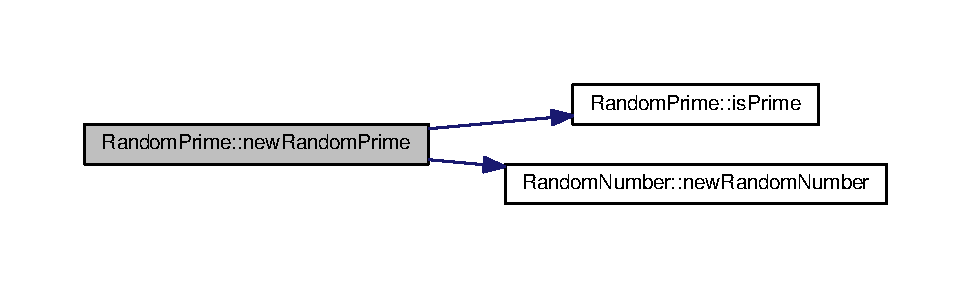
\includegraphics[width=350pt]{classRandomPrime_a322ce83f7af45e67d009ff3ed19d0047_cgraph}
\end{center}
\end{figure}




\subsection{Member Data Documentation}
\hypertarget{classRandomPrime_aed4cde44e5f33444c1d0e02d061a6a22}{\index{Random\+Prime@{Random\+Prime}!random\+Number@{random\+Number}}
\index{random\+Number@{random\+Number}!Random\+Prime@{Random\+Prime}}
\subsubsection[{random\+Number}]{\setlength{\rightskip}{0pt plus 5cm}{\bf Random\+Number}$\ast$ Random\+Prime\+::random\+Number}}\label{classRandomPrime_aed4cde44e5f33444c1d0e02d061a6a22}


Ponteiro para a classe que cria um número aleatório, primo ou não. 



Definition at line 35 of file Random\+Prime.\+h.



Referenced by $\sim$\+Random\+Prime().



The documentation for this class was generated from the following file\+:\begin{DoxyCompactItemize}
\item 
\hyperlink{RandomPrime_8h}{Random\+Prime.\+h}\end{DoxyCompactItemize}

\hypertarget{classReader}{\section{Reader$<$ Type\+Of\+Content $>$ Class Template Reference}
\label{classReader}\index{Reader$<$ Type\+Of\+Content $>$@{Reader$<$ Type\+Of\+Content $>$}}
}


{\ttfamily \#include $<$Reader.\+h$>$}

\subsection*{Public Member Functions}
\begin{DoxyCompactItemize}
\item 
\hyperlink{classReader_a8b5850f38fe8b78b426575da9c421ba3}{Reader} (\hyperlink{Main_8cpp_a4505c08c065b48840a30eedd9845cce2}{string} pattern\+File\+Name, \hyperlink{Main_8cpp_a4505c08c065b48840a30eedd9845cce2}{string} text\+File\+Name)
\item 
void \hyperlink{classReader_a481551db3ffcea967de48b4725cb8bcb}{print\+Files} ()
\item 
bool \hyperlink{classReader_a7fbe4bed605ebdd00ec00309cff2ca9d}{file\+Exist} (const \hyperlink{Reader_8h_a4505c08c065b48840a30eedd9845cce2}{std\+::string} \&name)
\item 
\hyperlink{classBox}{Box}$<$ Type\+Of\+Content $>$ $\ast$ \hyperlink{classReader_a8ef7d743eeaf83f2c47e56164145afb0}{files\+To\+Box} ()
\end{DoxyCompactItemize}
\subsection*{Public Attributes}
\begin{DoxyCompactItemize}
\item 
std\+::fstream \hyperlink{classReader_ab1b8cba2b947b66777f32cbf7743ba7e}{text\+File}
\begin{DoxyCompactList}\small\item\em arquivo que contem o texto \end{DoxyCompactList}\item 
std\+::fstream \hyperlink{classReader_ab38c2e4b4e9e31982fd77158fb88eeec}{pattern\+File}
\begin{DoxyCompactList}\small\item\em arquivo que contem o pattern \end{DoxyCompactList}\end{DoxyCompactItemize}


\subsection{Detailed Description}
\subsubsection*{template$<$typename Type\+Of\+Content$>$class Reader$<$ Type\+Of\+Content $>$}


\begin{DoxyTemplParams}{Template Parameters}
{\em Type\+Of\+Content} & tipo da letra do alfabeto utilizado. Tipo dos termos de text e pattern tipo usado para a leitura dos arquivos que contem o texto \\
\hline
\end{DoxyTemplParams}


Definition at line 45 of file Reader.\+h.



\subsection{Constructor \& Destructor Documentation}
\hypertarget{classReader_a8b5850f38fe8b78b426575da9c421ba3}{\index{Reader@{Reader}!Reader@{Reader}}
\index{Reader@{Reader}!Reader@{Reader}}
\subsubsection[{Reader}]{\setlength{\rightskip}{0pt plus 5cm}template$<$typename Type\+Of\+Content$>$ {\bf Reader}$<$ Type\+Of\+Content $>$\+::{\bf Reader} (
\begin{DoxyParamCaption}
\item[{{\bf string}}]{pattern\+File\+Name, }
\item[{{\bf string}}]{text\+File\+Name}
\end{DoxyParamCaption}
)\hspace{0.3cm}{\ttfamily [inline]}}}\label{classReader_a8b5850f38fe8b78b426575da9c421ba3}
Construtor que, atraves dos nomes dos arquivos, os abre. 
\begin{DoxyParams}{Parameters}
{\em pattern\+File\+Name} & nome do arquivo contendo pattern \\
\hline
{\em text\+File\+Name} & nome do arquivo contendo text \\
\hline
\end{DoxyParams}


Definition at line 60 of file Reader.\+h.



References Reader$<$ Type\+Of\+Content $>$\+::file\+Exist().



Here is the call graph for this function\+:\nopagebreak
\begin{figure}[H]
\begin{center}
\leavevmode
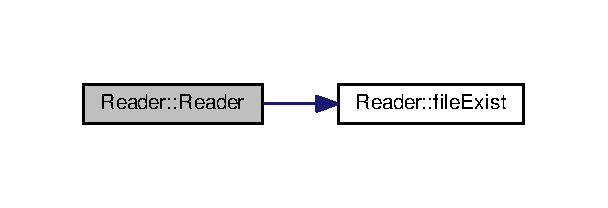
\includegraphics[width=292pt]{classReader_a8b5850f38fe8b78b426575da9c421ba3_cgraph}
\end{center}
\end{figure}




\subsection{Member Function Documentation}
\hypertarget{classReader_a7fbe4bed605ebdd00ec00309cff2ca9d}{\index{Reader@{Reader}!file\+Exist@{file\+Exist}}
\index{file\+Exist@{file\+Exist}!Reader@{Reader}}
\subsubsection[{file\+Exist}]{\setlength{\rightskip}{0pt plus 5cm}template$<$typename Type\+Of\+Content$>$ bool {\bf Reader}$<$ Type\+Of\+Content $>$\+::file\+Exist (
\begin{DoxyParamCaption}
\item[{const {\bf std\+::string} \&}]{name}
\end{DoxyParamCaption}
)\hspace{0.3cm}{\ttfamily [inline]}}}\label{classReader_a7fbe4bed605ebdd00ec00309cff2ca9d}


Definition at line 117 of file Reader.\+h.



Referenced by Reader$<$ Type\+Of\+Content $>$\+::\+Reader().

\hypertarget{classReader_a8ef7d743eeaf83f2c47e56164145afb0}{\index{Reader@{Reader}!files\+To\+Box@{files\+To\+Box}}
\index{files\+To\+Box@{files\+To\+Box}!Reader@{Reader}}
\subsubsection[{files\+To\+Box}]{\setlength{\rightskip}{0pt plus 5cm}template$<$typename Type\+Of\+Content$>$ {\bf Box}$<$Type\+Of\+Content$>$$\ast$ {\bf Reader}$<$ Type\+Of\+Content $>$\+::files\+To\+Box (
\begin{DoxyParamCaption}
{}
\end{DoxyParamCaption}
)\hspace{0.3cm}{\ttfamily [inline]}}}\label{classReader_a8ef7d743eeaf83f2c47e56164145afb0}
através dos arquivos encontrados no construtor, lê cada arquivo e para cada um adiciona seu respectivo conteúdo em um vetor de Letter$<$char$>$ diferente. Por fim, agrupa-\/os, junto aos seus tamanhos em um objeto do tipo \hyperlink{classBox}{Box} \begin{DoxyReturn}{Returns}
box contendo os vetores de Letter$<$char$>$ criados e seus tamanhos 
\end{DoxyReturn}
\begin{DoxySeeAlso}{See also}
\hyperlink{classLetter}{Letter} 

\hyperlink{classBox}{Box} 
\end{DoxySeeAlso}


Definition at line 141 of file Reader.\+h.



Referenced by main().

\hypertarget{classReader_a481551db3ffcea967de48b4725cb8bcb}{\index{Reader@{Reader}!print\+Files@{print\+Files}}
\index{print\+Files@{print\+Files}!Reader@{Reader}}
\subsubsection[{print\+Files}]{\setlength{\rightskip}{0pt plus 5cm}template$<$typename Type\+Of\+Content$>$ void {\bf Reader}$<$ Type\+Of\+Content $>$\+::print\+Files (
\begin{DoxyParamCaption}
{}
\end{DoxyParamCaption}
)\hspace{0.3cm}{\ttfamily [inline]}}}\label{classReader_a481551db3ffcea967de48b4725cb8bcb}
transforma os dados de um arquivo diretamente no tipo \hyperlink{classBox}{Box} Usado quando o dado a ser trabalho eh char. Quando for token, apos a leitura do arquivo eh necessario realizar um passo a mais para a tokenização \begin{DoxyReturn}{Returns}
void 
\end{DoxyReturn}


Definition at line 85 of file Reader.\+h.



\subsection{Member Data Documentation}
\hypertarget{classReader_ab38c2e4b4e9e31982fd77158fb88eeec}{\index{Reader@{Reader}!pattern\+File@{pattern\+File}}
\index{pattern\+File@{pattern\+File}!Reader@{Reader}}
\subsubsection[{pattern\+File}]{\setlength{\rightskip}{0pt plus 5cm}template$<$typename Type\+Of\+Content$>$ std\+::fstream {\bf Reader}$<$ Type\+Of\+Content $>$\+::pattern\+File}}\label{classReader_ab38c2e4b4e9e31982fd77158fb88eeec}


arquivo que contem o pattern 



Definition at line 53 of file Reader.\+h.

\hypertarget{classReader_ab1b8cba2b947b66777f32cbf7743ba7e}{\index{Reader@{Reader}!text\+File@{text\+File}}
\index{text\+File@{text\+File}!Reader@{Reader}}
\subsubsection[{text\+File}]{\setlength{\rightskip}{0pt plus 5cm}template$<$typename Type\+Of\+Content$>$ std\+::fstream {\bf Reader}$<$ Type\+Of\+Content $>$\+::text\+File}}\label{classReader_ab1b8cba2b947b66777f32cbf7743ba7e}


arquivo que contem o texto 



Definition at line 49 of file Reader.\+h.



The documentation for this class was generated from the following file\+:\begin{DoxyCompactItemize}
\item 
\hyperlink{Reader_8h}{Reader.\+h}\end{DoxyCompactItemize}

\hypertarget{classRKRGST}{\section{R\+K\+R\+G\+S\+T$<$ Type\+Of\+Content $>$ Class Template Reference}
\label{classRKRGST}\index{R\+K\+R\+G\+S\+T$<$ Type\+Of\+Content $>$@{R\+K\+R\+G\+S\+T$<$ Type\+Of\+Content $>$}}
}


{\ttfamily \#include $<$R\+K\+R\+G\+S\+T.\+h$>$}



Collaboration diagram for R\+K\+R\+G\+S\+T$<$ Type\+Of\+Content $>$\+:\nopagebreak
\begin{figure}[H]
\begin{center}
\leavevmode
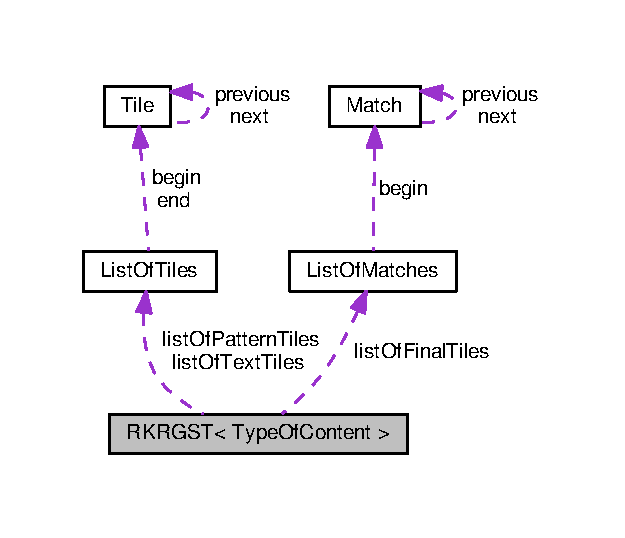
\includegraphics[width=300pt]{classRKRGST__coll__graph}
\end{center}
\end{figure}
\subsection*{Public Member Functions}
\begin{DoxyCompactItemize}
\item 
\hyperlink{classRKRGST_a66390e97e207872a55ea6ee0d3b2c0ee}{R\+K\+R\+G\+S\+T} (\hyperlink{classBox}{Box}$<$ Type\+Of\+Content $>$ $\ast$\hyperlink{classRKRGST_ae0737f82fb5c44b9edd663a9ed00a7fe}{box}, int \hyperlink{classRKRGST_ad4e450cff7656afab26be8eb27c4f87c}{initial\+Search\+Length}, int \hyperlink{classRKRGST_aaf28410e7b3c34bcfbffd17cd0d014b2}{minimum\+Search\+Length}, int \hyperlink{classRKRGST_a49054fd9d1f1fc34a5c2dedaba5e6f14}{base\+Length})
\item 
void \hyperlink{classRKRGST_aef01e8fd6c0e17482724c0f3fd7ad89f}{execute} ()
\item 
void \hyperlink{classRKRGST_a469647a68dc845b14b01d37505eee6d1}{mark\+Arrays} (int search\+Length, \hyperlink{classListOfMatches}{List\+Of\+Matches} $\ast$list\+Of\+Matches)
\item 
int \hyperlink{classRKRGST_a4ef9cf20505986d0f023a5384fdf844c}{scan\+Pattern} (int search\+Length, \hyperlink{classListOfMatches}{List\+Of\+Matches} $\ast$list\+Of\+Matches)
\item 
int \hyperlink{classRKRGST_a37cf8598f504f175035a83a69cfeaa08}{find\+Pattern\+Substring} (int search\+Length, \hyperlink{classHashTable}{Hash\+Table}$<$ Type\+Of\+Content $>$ $\ast$text\+Hash\+Table, int actual\+Index)
\item 
void \hyperlink{classRKRGST_a12e85e53ee2298818cead4ffe76eb8b3}{fill\+Text\+Hash\+Table} (int search\+Length, \hyperlink{classHashTable}{Hash\+Table}$<$ Type\+Of\+Content $>$ $\ast$text\+Hash\+Table)
\item 
bool \hyperlink{classRKRGST_aa2b3943e1897025c9f8293ee98edabca}{occluded} (\hyperlink{classBox}{Box}$<$ Type\+Of\+Content $>$ $\ast$\hyperlink{classRKRGST_ae0737f82fb5c44b9edd663a9ed00a7fe}{box}, \hyperlink{classMatch}{Match} $\ast$match)
\item 
void \hyperlink{classRKRGST_af44ddce704c698ee3cb38a7262a36874}{mark\+Tokens} (\hyperlink{classBox}{Box}$<$ Type\+Of\+Content $>$ $\ast$\hyperlink{classRKRGST_ae0737f82fb5c44b9edd663a9ed00a7fe}{box}, \hyperlink{classMatch}{Match} $\ast$match)
\end{DoxyCompactItemize}
\subsection*{Public Attributes}
\begin{DoxyCompactItemize}
\item 
int \hyperlink{classRKRGST_ad4e450cff7656afab26be8eb27c4f87c}{initial\+Search\+Length}
\begin{DoxyCompactList}\small\item\em Tamanho inicial do padrão buscado. \end{DoxyCompactList}\item 
int \hyperlink{classRKRGST_aaf28410e7b3c34bcfbffd17cd0d014b2}{minimum\+Search\+Length}
\begin{DoxyCompactList}\small\item\em Tamanho mínimo a ser buscado. \end{DoxyCompactList}\item 
int \hyperlink{classRKRGST_aea66b780697be63c91342029335ad8ef}{prime\+Number}
\begin{DoxyCompactList}\small\item\em Número primo utilizado na hash. \end{DoxyCompactList}\item 
\hyperlink{classBox}{Box}$<$ Type\+Of\+Content $>$ $\ast$ \hyperlink{classRKRGST_ae0737f82fb5c44b9edd663a9ed00a7fe}{box}
\begin{DoxyCompactList}\small\item\em Container de dados que guarda a palavra que compõe a Text, a palavra que contém a Pattern e seus respectivos tamanhos. \end{DoxyCompactList}\item 
\hyperlink{classListOfTiles}{List\+Of\+Tiles} $\ast$ \hyperlink{classRKRGST_ad2335f6d83faf621a99b66c680f32b5d}{list\+Of\+Pattern\+Tiles}
\begin{DoxyCompactList}\small\item\em Ponteiro para um objeto da classe \hyperlink{classListOfTiles}{List\+Of\+Tiles} que contém uma lista de objetos da classe \hyperlink{classTile}{Tile} relativos à Pattern. \end{DoxyCompactList}\item 
\hyperlink{classListOfTiles}{List\+Of\+Tiles} $\ast$ \hyperlink{classRKRGST_a03afdb90a534a2420da654ddadb032c2}{list\+Of\+Text\+Tiles}
\begin{DoxyCompactList}\small\item\em Ponteiro para um objeto da classe \hyperlink{classListOfTiles}{List\+Of\+Tiles} que contém uma lista de objetos da classe \hyperlink{classTile}{Tile} relativos à Text. \end{DoxyCompactList}\item 
int \hyperlink{classRKRGST_a49054fd9d1f1fc34a5c2dedaba5e6f14}{base\+Length}
\begin{DoxyCompactList}\small\item\em Tamanho da base dos números gerados pela \hyperlink{classRollingHash}{Rolling\+Hash}. \end{DoxyCompactList}\item 
int \hyperlink{classRKRGST_aaebf5b2da8490b6fc1ea06300914256e}{length\+Of\+Tokens\+Tiled}
\item 
\hyperlink{classListOfMatches}{List\+Of\+Matches} $\ast$ \hyperlink{classRKRGST_a1ae736b742c0cbcdd6d30c5201d4181b}{list\+Of\+Final\+Tiles}
\end{DoxyCompactItemize}


\subsection{Detailed Description}
\subsubsection*{template$<$typename Type\+Of\+Content$>$class R\+K\+R\+G\+S\+T$<$ Type\+Of\+Content $>$}


\begin{DoxyTemplParams}{Template Parameters}
{\em Type\+Of\+Content} & tipo da letra do alfabeto utilizado. Tipo dos termos da pattern e da text Classe contendo todos os algoritmos realizados pelo \hyperlink{classRKRGST}{R\+K\+R\+G\+S\+T} \\
\hline
\end{DoxyTemplParams}


Definition at line 48 of file R\+K\+R\+G\+S\+T.\+h.



\subsection{Constructor \& Destructor Documentation}
\hypertarget{classRKRGST_a66390e97e207872a55ea6ee0d3b2c0ee}{\index{R\+K\+R\+G\+S\+T@{R\+K\+R\+G\+S\+T}!R\+K\+R\+G\+S\+T@{R\+K\+R\+G\+S\+T}}
\index{R\+K\+R\+G\+S\+T@{R\+K\+R\+G\+S\+T}!R\+K\+R\+G\+S\+T@{R\+K\+R\+G\+S\+T}}
\subsubsection[{R\+K\+R\+G\+S\+T}]{\setlength{\rightskip}{0pt plus 5cm}template$<$typename Type\+Of\+Content$>$ {\bf R\+K\+R\+G\+S\+T}$<$ Type\+Of\+Content $>$\+::{\bf R\+K\+R\+G\+S\+T} (
\begin{DoxyParamCaption}
\item[{{\bf Box}$<$ Type\+Of\+Content $>$ $\ast$}]{box, }
\item[{int}]{initial\+Search\+Length, }
\item[{int}]{minimum\+Search\+Length, }
\item[{int}]{base\+Length}
\end{DoxyParamCaption}
)\hspace{0.3cm}{\ttfamily [inline]}}}\label{classRKRGST_a66390e97e207872a55ea6ee0d3b2c0ee}
Construtor de objeto da classe \hyperlink{classRKRGST}{R\+K\+R\+G\+S\+T} 
\begin{DoxyParams}{Parameters}
{\em box} & Container de dados que guarda a palavra que compõe a Text, a palavra que contém a Pattern e seus respectivos tamanhos \\
\hline
{\em initial\+Search\+Length} & Tamanho inicial do padrão buscado \\
\hline
{\em minimum\+Search\+Length} & Tamanho mínimo a ser buscado \\
\hline
{\em base\+Length} & Tamanho da base dos números gerados pela \hyperlink{classRollingHash}{Rolling\+Hash}. \\
\hline
\end{DoxyParams}


Definition at line 86 of file R\+K\+R\+G\+S\+T.\+h.



References R\+K\+R\+G\+S\+T$<$ Type\+Of\+Content $>$\+::base\+Length, R\+K\+R\+G\+S\+T$<$ Type\+Of\+Content $>$\+::box, R\+K\+R\+G\+S\+T$<$ Type\+Of\+Content $>$\+::initial\+Search\+Length, R\+K\+R\+G\+S\+T$<$ Type\+Of\+Content $>$\+::minimum\+Search\+Length, and Random\+Prime\+::new\+Random\+Prime().



Here is the call graph for this function\+:\nopagebreak
\begin{figure}[H]
\begin{center}
\leavevmode
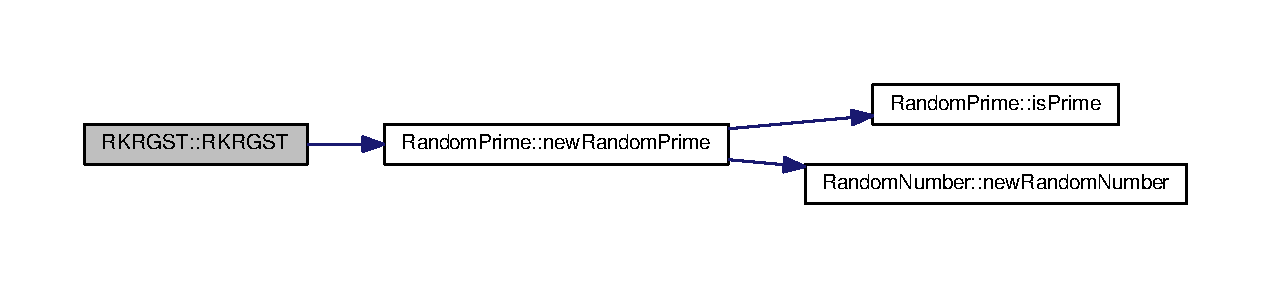
\includegraphics[width=350pt]{classRKRGST_a66390e97e207872a55ea6ee0d3b2c0ee_cgraph}
\end{center}
\end{figure}




\subsection{Member Function Documentation}
\hypertarget{classRKRGST_aef01e8fd6c0e17482724c0f3fd7ad89f}{\index{R\+K\+R\+G\+S\+T@{R\+K\+R\+G\+S\+T}!execute@{execute}}
\index{execute@{execute}!R\+K\+R\+G\+S\+T@{R\+K\+R\+G\+S\+T}}
\subsubsection[{execute}]{\setlength{\rightskip}{0pt plus 5cm}template$<$typename Type\+Of\+Content$>$ void {\bf R\+K\+R\+G\+S\+T}$<$ Type\+Of\+Content $>$\+::execute (
\begin{DoxyParamCaption}
{}
\end{DoxyParamCaption}
)\hspace{0.3cm}{\ttfamily [inline]}}}\label{classRKRGST_aef01e8fd6c0e17482724c0f3fd7ad89f}
Método que executa t odo o algoritmo \hyperlink{classRKRGST}{R\+K\+R\+G\+S\+T} 

Definition at line 104 of file R\+K\+R\+G\+S\+T.\+h.



References R\+K\+R\+G\+S\+T$<$ Type\+Of\+Content $>$\+::initial\+Search\+Length, R\+K\+R\+G\+S\+T$<$ Type\+Of\+Content $>$\+::mark\+Arrays(), M\+A\+X\+\_\+\+L\+E\+N\+G\+T\+H, R\+K\+R\+G\+S\+T$<$ Type\+Of\+Content $>$\+::minimum\+Search\+Length, and R\+K\+R\+G\+S\+T$<$ Type\+Of\+Content $>$\+::scan\+Pattern().



Referenced by main().



Here is the call graph for this function\+:\nopagebreak
\begin{figure}[H]
\begin{center}
\leavevmode
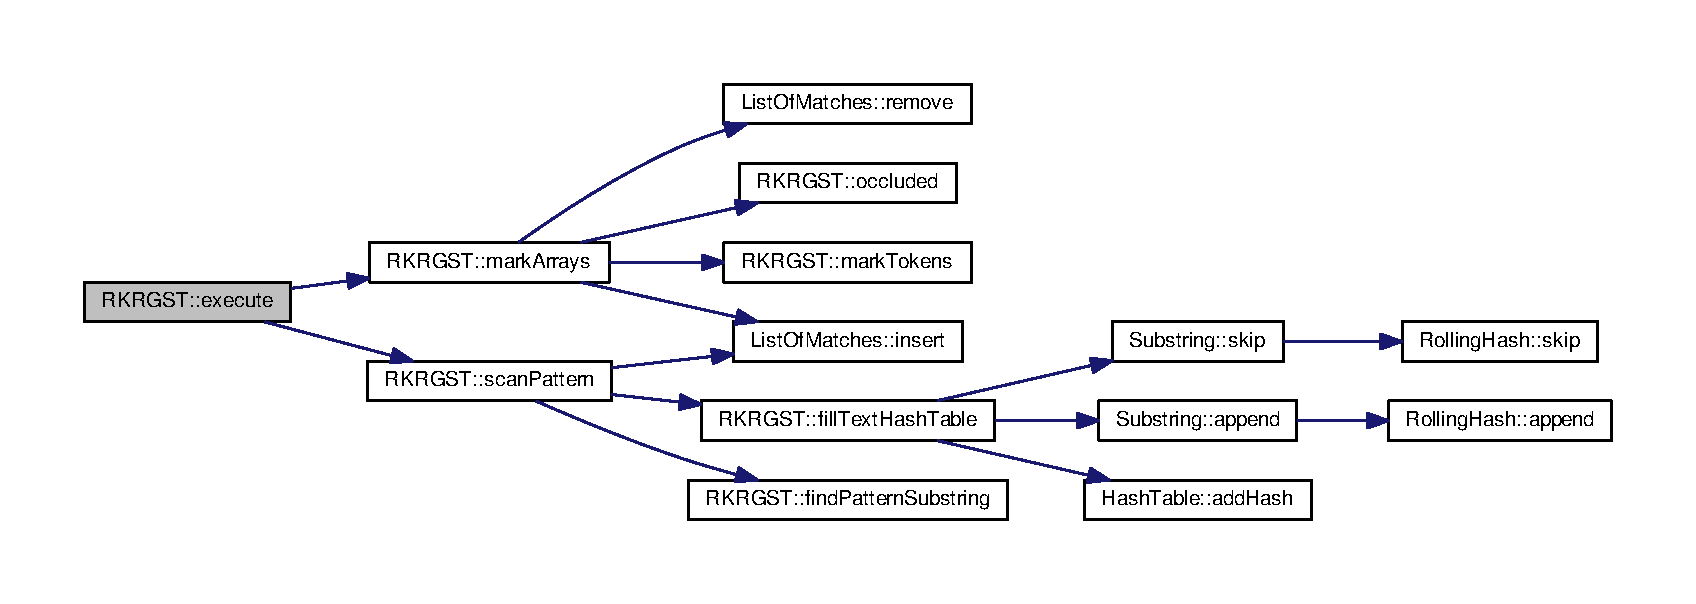
\includegraphics[width=350pt]{classRKRGST_aef01e8fd6c0e17482724c0f3fd7ad89f_cgraph}
\end{center}
\end{figure}


\hypertarget{classRKRGST_a12e85e53ee2298818cead4ffe76eb8b3}{\index{R\+K\+R\+G\+S\+T@{R\+K\+R\+G\+S\+T}!fill\+Text\+Hash\+Table@{fill\+Text\+Hash\+Table}}
\index{fill\+Text\+Hash\+Table@{fill\+Text\+Hash\+Table}!R\+K\+R\+G\+S\+T@{R\+K\+R\+G\+S\+T}}
\subsubsection[{fill\+Text\+Hash\+Table}]{\setlength{\rightskip}{0pt plus 5cm}template$<$typename Type\+Of\+Content$>$ void {\bf R\+K\+R\+G\+S\+T}$<$ Type\+Of\+Content $>$\+::fill\+Text\+Hash\+Table (
\begin{DoxyParamCaption}
\item[{int}]{search\+Length, }
\item[{{\bf Hash\+Table}$<$ Type\+Of\+Content $>$ $\ast$}]{text\+Hash\+Table}
\end{DoxyParamCaption}
)\hspace{0.3cm}{\ttfamily [inline]}}}\label{classRKRGST_a12e85e53ee2298818cead4ffe76eb8b3}
Preenche a tabela de hash do texto com todas as substrings de tamanho search\+Length não marcadas 
\begin{DoxyParams}{Parameters}
{\em search\+Length} & Tamanho das substrings buscadas. \\
\hline
{\em text\+Hash\+Table} & Tabela de Hash das subcadeias de text. \\
\hline
\end{DoxyParams}
\begin{DoxySeeAlso}{See also}
\hyperlink{classHashTable}{Hash\+Table} 
\end{DoxySeeAlso}


Definition at line 397 of file R\+K\+R\+G\+S\+T.\+h.



References Hash\+Table$<$ Type\+Of\+Content $>$\+::add\+Hash(), Substring$<$ Type\+Of\+Content $>$\+::append(), R\+K\+R\+G\+S\+T$<$ Type\+Of\+Content $>$\+::base\+Length, Tile\+::begin, List\+Of\+Tiles\+::begin, Substring$<$ Type\+Of\+Content $>$\+::begin, Tile\+::end, Substring$<$ Type\+Of\+Content $>$\+::end, Tile\+::next, Substring$<$ Type\+Of\+Content $>$\+::next, Substring$<$ Type\+Of\+Content $>$\+::previous, R\+K\+R\+G\+S\+T$<$ Type\+Of\+Content $>$\+::prime\+Number, Substring$<$ Type\+Of\+Content $>$\+::rolling\+Hash, Substring$<$ Type\+Of\+Content $>$\+::skip(), Substring$<$ Type\+Of\+Content $>$\+::string, Box$<$ Type\+Of\+Content $>$\+::text, and Box$<$ Type\+Of\+Content $>$\+::text\+Size.



Referenced by R\+K\+R\+G\+S\+T$<$ Type\+Of\+Content $>$\+::scan\+Pattern().



Here is the call graph for this function\+:\nopagebreak
\begin{figure}[H]
\begin{center}
\leavevmode
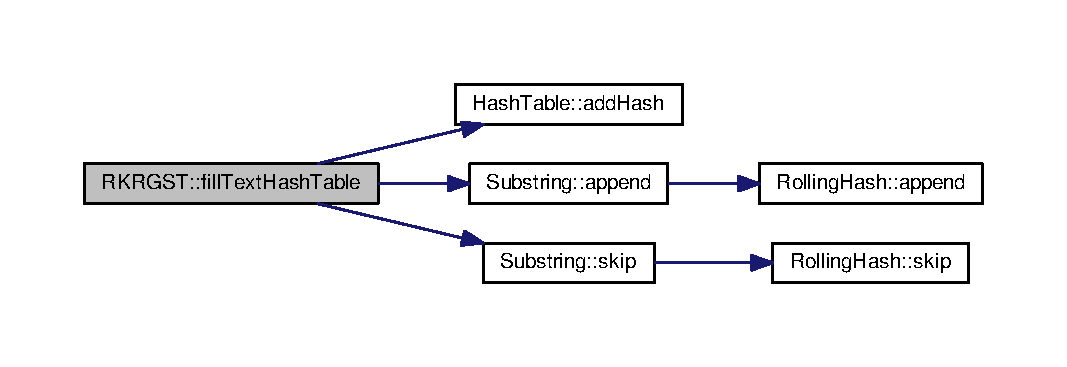
\includegraphics[width=350pt]{classRKRGST_a12e85e53ee2298818cead4ffe76eb8b3_cgraph}
\end{center}
\end{figure}


\hypertarget{classRKRGST_a37cf8598f504f175035a83a69cfeaa08}{\index{R\+K\+R\+G\+S\+T@{R\+K\+R\+G\+S\+T}!find\+Pattern\+Substring@{find\+Pattern\+Substring}}
\index{find\+Pattern\+Substring@{find\+Pattern\+Substring}!R\+K\+R\+G\+S\+T@{R\+K\+R\+G\+S\+T}}
\subsubsection[{find\+Pattern\+Substring}]{\setlength{\rightskip}{0pt plus 5cm}template$<$typename Type\+Of\+Content$>$ int {\bf R\+K\+R\+G\+S\+T}$<$ Type\+Of\+Content $>$\+::find\+Pattern\+Substring (
\begin{DoxyParamCaption}
\item[{int}]{search\+Length, }
\item[{{\bf Hash\+Table}$<$ Type\+Of\+Content $>$ $\ast$}]{text\+Hash\+Table, }
\item[{int}]{actual\+Index}
\end{DoxyParamCaption}
)\hspace{0.3cm}{\ttfamily [inline]}}}\label{classRKRGST_a37cf8598f504f175035a83a69cfeaa08}
Encontra o índice do início de uma substring de tamanho search\+Length. Nenhuma as suas letras podem estar marcadas. 
\begin{DoxyParams}{Parameters}
{\em search\+Length} & Tamanho das substrings buscadas. \\
\hline
{\em text\+Hash\+Table} & Tabela de Hash das subcadeias de text. \\
\hline
{\em actual\+Index} & indice da letra do pattern \\
\hline
\end{DoxyParams}
\begin{DoxyReturn}{Returns}
Retorna o índice inicial da substring ou -\/1 caso não haja substring de tamanho search\+Length sem letras marcadas. 
\end{DoxyReturn}


Definition at line 319 of file R\+K\+R\+G\+S\+T.\+h.



References Tile\+::begin, List\+Of\+Tiles\+::begin, Tile\+::end, Tile\+::next, Box$<$ Type\+Of\+Content $>$\+::pattern, and Box$<$ Type\+Of\+Content $>$\+::pattern\+Size.



Referenced by R\+K\+R\+G\+S\+T$<$ Type\+Of\+Content $>$\+::scan\+Pattern().

\hypertarget{classRKRGST_a469647a68dc845b14b01d37505eee6d1}{\index{R\+K\+R\+G\+S\+T@{R\+K\+R\+G\+S\+T}!mark\+Arrays@{mark\+Arrays}}
\index{mark\+Arrays@{mark\+Arrays}!R\+K\+R\+G\+S\+T@{R\+K\+R\+G\+S\+T}}
\subsubsection[{mark\+Arrays}]{\setlength{\rightskip}{0pt plus 5cm}template$<$typename Type\+Of\+Content$>$ void {\bf R\+K\+R\+G\+S\+T}$<$ Type\+Of\+Content $>$\+::mark\+Arrays (
\begin{DoxyParamCaption}
\item[{int}]{search\+Length, }
\item[{{\bf List\+Of\+Matches} $\ast$}]{list\+Of\+Matches}
\end{DoxyParamCaption}
)\hspace{0.3cm}{\ttfamily [inline]}}}\label{classRKRGST_a469647a68dc845b14b01d37505eee6d1}
Método que marca as letras de um casamento 
\begin{DoxyParams}{Parameters}
{\em search\+Length} & Tamanho do casamento. \\
\hline
{\em list\+Of\+Matches} & Casamentos a serem marcados. \\
\hline
\end{DoxyParams}


Definition at line 157 of file R\+K\+R\+G\+S\+T.\+h.



References List\+Of\+Matches\+::insert(), Match\+::length, R\+K\+R\+G\+S\+T$<$ Type\+Of\+Content $>$\+::mark\+Tokens(), List\+Of\+Matches\+::number\+Of\+Matches, R\+K\+R\+G\+S\+T$<$ Type\+Of\+Content $>$\+::occluded(), Match\+::pattern\+Index, List\+Of\+Matches\+::remove(), and Match\+::text\+Index.



Referenced by R\+K\+R\+G\+S\+T$<$ Type\+Of\+Content $>$\+::execute().



Here is the call graph for this function\+:\nopagebreak
\begin{figure}[H]
\begin{center}
\leavevmode
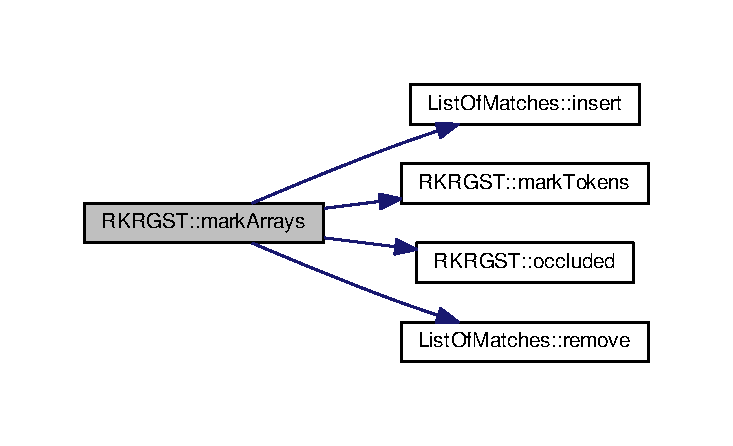
\includegraphics[width=350pt]{classRKRGST_a469647a68dc845b14b01d37505eee6d1_cgraph}
\end{center}
\end{figure}


\hypertarget{classRKRGST_af44ddce704c698ee3cb38a7262a36874}{\index{R\+K\+R\+G\+S\+T@{R\+K\+R\+G\+S\+T}!mark\+Tokens@{mark\+Tokens}}
\index{mark\+Tokens@{mark\+Tokens}!R\+K\+R\+G\+S\+T@{R\+K\+R\+G\+S\+T}}
\subsubsection[{mark\+Tokens}]{\setlength{\rightskip}{0pt plus 5cm}template$<$typename Type\+Of\+Content$>$ void {\bf R\+K\+R\+G\+S\+T}$<$ Type\+Of\+Content $>$\+::mark\+Tokens (
\begin{DoxyParamCaption}
\item[{{\bf Box}$<$ Type\+Of\+Content $>$ $\ast$}]{box, }
\item[{{\bf Match} $\ast$}]{match}
\end{DoxyParamCaption}
)\hspace{0.3cm}{\ttfamily [inline]}}}\label{classRKRGST_af44ddce704c698ee3cb38a7262a36874}
Marca os tokens de um casamento 
\begin{DoxyParams}{Parameters}
{\em box} & Objeto contendo text, pattern e seus respectivos tamanhos. \\
\hline
{\em match} & Casamento a ser marcado \\
\hline
\end{DoxyParams}


Definition at line 637 of file R\+K\+R\+G\+S\+T.\+h.



References Match\+::length, Box$<$ Type\+Of\+Content $>$\+::pattern, Match\+::pattern\+Index, Box$<$ Type\+Of\+Content $>$\+::text, and Match\+::text\+Index.



Referenced by R\+K\+R\+G\+S\+T$<$ Type\+Of\+Content $>$\+::mark\+Arrays().

\hypertarget{classRKRGST_aa2b3943e1897025c9f8293ee98edabca}{\index{R\+K\+R\+G\+S\+T@{R\+K\+R\+G\+S\+T}!occluded@{occluded}}
\index{occluded@{occluded}!R\+K\+R\+G\+S\+T@{R\+K\+R\+G\+S\+T}}
\subsubsection[{occluded}]{\setlength{\rightskip}{0pt plus 5cm}template$<$typename Type\+Of\+Content$>$ bool {\bf R\+K\+R\+G\+S\+T}$<$ Type\+Of\+Content $>$\+::occluded (
\begin{DoxyParamCaption}
\item[{{\bf Box}$<$ Type\+Of\+Content $>$ $\ast$}]{box, }
\item[{{\bf Match} $\ast$}]{match}
\end{DoxyParamCaption}
)\hspace{0.3cm}{\ttfamily [inline]}}}\label{classRKRGST_aa2b3943e1897025c9f8293ee98edabca}
Verifica se o casamento é ocluso por algum tile. 
\begin{DoxyParams}{Parameters}
{\em box} & Objeto contendo text, pattern e seus respectivos tamanhos. \\
\hline
{\em match} & Casamento a ser verificado \\
\hline
\end{DoxyParams}


Definition at line 616 of file R\+K\+R\+G\+S\+T.\+h.



References Match\+::length, Box$<$ Type\+Of\+Content $>$\+::pattern, Match\+::pattern\+Index, Box$<$ Type\+Of\+Content $>$\+::text, and Match\+::text\+Index.



Referenced by R\+K\+R\+G\+S\+T$<$ Type\+Of\+Content $>$\+::mark\+Arrays().

\hypertarget{classRKRGST_a4ef9cf20505986d0f023a5384fdf844c}{\index{R\+K\+R\+G\+S\+T@{R\+K\+R\+G\+S\+T}!scan\+Pattern@{scan\+Pattern}}
\index{scan\+Pattern@{scan\+Pattern}!R\+K\+R\+G\+S\+T@{R\+K\+R\+G\+S\+T}}
\subsubsection[{scan\+Pattern}]{\setlength{\rightskip}{0pt plus 5cm}template$<$typename Type\+Of\+Content$>$ int {\bf R\+K\+R\+G\+S\+T}$<$ Type\+Of\+Content $>$\+::scan\+Pattern (
\begin{DoxyParamCaption}
\item[{int}]{search\+Length, }
\item[{{\bf List\+Of\+Matches} $\ast$}]{list\+Of\+Matches}
\end{DoxyParamCaption}
)\hspace{0.3cm}{\ttfamily [inline]}}}\label{classRKRGST_a4ef9cf20505986d0f023a5384fdf844c}
Buscando casamentos de tamanho search\+Length 
\begin{DoxyParams}{Parameters}
{\em search\+Length} & Tamanho do casamento sendo buscado. \\
\hline
{\em list\+Of\+Matches} & Lista de casamentos encontrados na scan\+Pattern. \\
\hline
\end{DoxyParams}
Tabela de Hash contendo as substrings de Text 

Definition at line 190 of file R\+K\+R\+G\+S\+T.\+h.



References R\+K\+R\+G\+S\+T$<$ Type\+Of\+Content $>$\+::base\+Length, Substring$<$ Type\+Of\+Content $>$\+::begin, R\+K\+R\+G\+S\+T$<$ Type\+Of\+Content $>$\+::fill\+Text\+Hash\+Table(), R\+K\+R\+G\+S\+T$<$ Type\+Of\+Content $>$\+::find\+Pattern\+Substring(), List\+Of\+Matches\+::insert(), M\+A\+X\+\_\+\+L\+E\+N\+G\+T\+H, Substring$<$ Type\+Of\+Content $>$\+::next, Box$<$ Type\+Of\+Content $>$\+::pattern, Box$<$ Type\+Of\+Content $>$\+::pattern\+Size, R\+K\+R\+G\+S\+T$<$ Type\+Of\+Content $>$\+::prime\+Number, Substring$<$ Type\+Of\+Content $>$\+::rolling\+Hash, Substring$<$ Type\+Of\+Content $>$\+::string, Hash\+Table$<$ Type\+Of\+Content $>$\+::table, and Box$<$ Type\+Of\+Content $>$\+::text\+Size.



Referenced by R\+K\+R\+G\+S\+T$<$ Type\+Of\+Content $>$\+::execute().



Here is the call graph for this function\+:\nopagebreak
\begin{figure}[H]
\begin{center}
\leavevmode
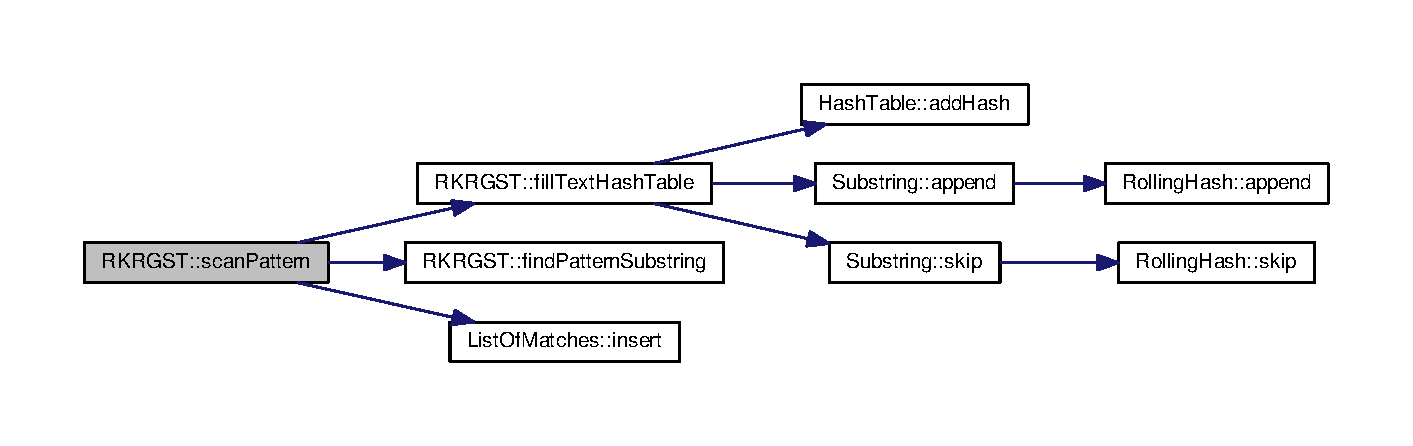
\includegraphics[width=350pt]{classRKRGST_a4ef9cf20505986d0f023a5384fdf844c_cgraph}
\end{center}
\end{figure}




\subsection{Member Data Documentation}
\hypertarget{classRKRGST_a49054fd9d1f1fc34a5c2dedaba5e6f14}{\index{R\+K\+R\+G\+S\+T@{R\+K\+R\+G\+S\+T}!base\+Length@{base\+Length}}
\index{base\+Length@{base\+Length}!R\+K\+R\+G\+S\+T@{R\+K\+R\+G\+S\+T}}
\subsubsection[{base\+Length}]{\setlength{\rightskip}{0pt plus 5cm}template$<$typename Type\+Of\+Content$>$ int {\bf R\+K\+R\+G\+S\+T}$<$ Type\+Of\+Content $>$\+::base\+Length}}\label{classRKRGST_a49054fd9d1f1fc34a5c2dedaba5e6f14}


Tamanho da base dos números gerados pela \hyperlink{classRollingHash}{Rolling\+Hash}. 



Definition at line 71 of file R\+K\+R\+G\+S\+T.\+h.



Referenced by R\+K\+R\+G\+S\+T$<$ Type\+Of\+Content $>$\+::fill\+Text\+Hash\+Table(), R\+K\+R\+G\+S\+T$<$ Type\+Of\+Content $>$\+::\+R\+K\+R\+G\+S\+T(), and R\+K\+R\+G\+S\+T$<$ Type\+Of\+Content $>$\+::scan\+Pattern().

\hypertarget{classRKRGST_ae0737f82fb5c44b9edd663a9ed00a7fe}{\index{R\+K\+R\+G\+S\+T@{R\+K\+R\+G\+S\+T}!box@{box}}
\index{box@{box}!R\+K\+R\+G\+S\+T@{R\+K\+R\+G\+S\+T}}
\subsubsection[{box}]{\setlength{\rightskip}{0pt plus 5cm}template$<$typename Type\+Of\+Content$>$ {\bf Box}$<$ Type\+Of\+Content $>$$\ast$ {\bf R\+K\+R\+G\+S\+T}$<$ Type\+Of\+Content $>$\+::box}}\label{classRKRGST_ae0737f82fb5c44b9edd663a9ed00a7fe}


Container de dados que guarda a palavra que compõe a Text, a palavra que contém a Pattern e seus respectivos tamanhos. 



Definition at line 62 of file R\+K\+R\+G\+S\+T.\+h.



Referenced by R\+K\+R\+G\+S\+T$<$ Type\+Of\+Content $>$\+::\+R\+K\+R\+G\+S\+T().

\hypertarget{classRKRGST_ad4e450cff7656afab26be8eb27c4f87c}{\index{R\+K\+R\+G\+S\+T@{R\+K\+R\+G\+S\+T}!initial\+Search\+Length@{initial\+Search\+Length}}
\index{initial\+Search\+Length@{initial\+Search\+Length}!R\+K\+R\+G\+S\+T@{R\+K\+R\+G\+S\+T}}
\subsubsection[{initial\+Search\+Length}]{\setlength{\rightskip}{0pt plus 5cm}template$<$typename Type\+Of\+Content$>$ int {\bf R\+K\+R\+G\+S\+T}$<$ Type\+Of\+Content $>$\+::initial\+Search\+Length}}\label{classRKRGST_ad4e450cff7656afab26be8eb27c4f87c}


Tamanho inicial do padrão buscado. 



Definition at line 54 of file R\+K\+R\+G\+S\+T.\+h.



Referenced by R\+K\+R\+G\+S\+T$<$ Type\+Of\+Content $>$\+::execute(), and R\+K\+R\+G\+S\+T$<$ Type\+Of\+Content $>$\+::\+R\+K\+R\+G\+S\+T().

\hypertarget{classRKRGST_aaebf5b2da8490b6fc1ea06300914256e}{\index{R\+K\+R\+G\+S\+T@{R\+K\+R\+G\+S\+T}!length\+Of\+Tokens\+Tiled@{length\+Of\+Tokens\+Tiled}}
\index{length\+Of\+Tokens\+Tiled@{length\+Of\+Tokens\+Tiled}!R\+K\+R\+G\+S\+T@{R\+K\+R\+G\+S\+T}}
\subsubsection[{length\+Of\+Tokens\+Tiled}]{\setlength{\rightskip}{0pt plus 5cm}template$<$typename Type\+Of\+Content$>$ int {\bf R\+K\+R\+G\+S\+T}$<$ Type\+Of\+Content $>$\+::length\+Of\+Tokens\+Tiled}}\label{classRKRGST_aaebf5b2da8490b6fc1ea06300914256e}


Definition at line 73 of file R\+K\+R\+G\+S\+T.\+h.



Referenced by main().

\hypertarget{classRKRGST_a1ae736b742c0cbcdd6d30c5201d4181b}{\index{R\+K\+R\+G\+S\+T@{R\+K\+R\+G\+S\+T}!list\+Of\+Final\+Tiles@{list\+Of\+Final\+Tiles}}
\index{list\+Of\+Final\+Tiles@{list\+Of\+Final\+Tiles}!R\+K\+R\+G\+S\+T@{R\+K\+R\+G\+S\+T}}
\subsubsection[{list\+Of\+Final\+Tiles}]{\setlength{\rightskip}{0pt plus 5cm}template$<$typename Type\+Of\+Content$>$ {\bf List\+Of\+Matches}$\ast$ {\bf R\+K\+R\+G\+S\+T}$<$ Type\+Of\+Content $>$\+::list\+Of\+Final\+Tiles}}\label{classRKRGST_a1ae736b742c0cbcdd6d30c5201d4181b}


Definition at line 75 of file R\+K\+R\+G\+S\+T.\+h.



Referenced by main().

\hypertarget{classRKRGST_ad2335f6d83faf621a99b66c680f32b5d}{\index{R\+K\+R\+G\+S\+T@{R\+K\+R\+G\+S\+T}!list\+Of\+Pattern\+Tiles@{list\+Of\+Pattern\+Tiles}}
\index{list\+Of\+Pattern\+Tiles@{list\+Of\+Pattern\+Tiles}!R\+K\+R\+G\+S\+T@{R\+K\+R\+G\+S\+T}}
\subsubsection[{list\+Of\+Pattern\+Tiles}]{\setlength{\rightskip}{0pt plus 5cm}template$<$typename Type\+Of\+Content$>$ {\bf List\+Of\+Tiles}$\ast$ {\bf R\+K\+R\+G\+S\+T}$<$ Type\+Of\+Content $>$\+::list\+Of\+Pattern\+Tiles}}\label{classRKRGST_ad2335f6d83faf621a99b66c680f32b5d}


Ponteiro para um objeto da classe \hyperlink{classListOfTiles}{List\+Of\+Tiles} que contém uma lista de objetos da classe \hyperlink{classTile}{Tile} relativos à Pattern. 



Definition at line 65 of file R\+K\+R\+G\+S\+T.\+h.

\hypertarget{classRKRGST_a03afdb90a534a2420da654ddadb032c2}{\index{R\+K\+R\+G\+S\+T@{R\+K\+R\+G\+S\+T}!list\+Of\+Text\+Tiles@{list\+Of\+Text\+Tiles}}
\index{list\+Of\+Text\+Tiles@{list\+Of\+Text\+Tiles}!R\+K\+R\+G\+S\+T@{R\+K\+R\+G\+S\+T}}
\subsubsection[{list\+Of\+Text\+Tiles}]{\setlength{\rightskip}{0pt plus 5cm}template$<$typename Type\+Of\+Content$>$ {\bf List\+Of\+Tiles}$\ast$ {\bf R\+K\+R\+G\+S\+T}$<$ Type\+Of\+Content $>$\+::list\+Of\+Text\+Tiles}}\label{classRKRGST_a03afdb90a534a2420da654ddadb032c2}


Ponteiro para um objeto da classe \hyperlink{classListOfTiles}{List\+Of\+Tiles} que contém uma lista de objetos da classe \hyperlink{classTile}{Tile} relativos à Text. 



Definition at line 68 of file R\+K\+R\+G\+S\+T.\+h.

\hypertarget{classRKRGST_aaf28410e7b3c34bcfbffd17cd0d014b2}{\index{R\+K\+R\+G\+S\+T@{R\+K\+R\+G\+S\+T}!minimum\+Search\+Length@{minimum\+Search\+Length}}
\index{minimum\+Search\+Length@{minimum\+Search\+Length}!R\+K\+R\+G\+S\+T@{R\+K\+R\+G\+S\+T}}
\subsubsection[{minimum\+Search\+Length}]{\setlength{\rightskip}{0pt plus 5cm}template$<$typename Type\+Of\+Content$>$ int {\bf R\+K\+R\+G\+S\+T}$<$ Type\+Of\+Content $>$\+::minimum\+Search\+Length}}\label{classRKRGST_aaf28410e7b3c34bcfbffd17cd0d014b2}


Tamanho mínimo a ser buscado. 



Definition at line 56 of file R\+K\+R\+G\+S\+T.\+h.



Referenced by R\+K\+R\+G\+S\+T$<$ Type\+Of\+Content $>$\+::execute(), and R\+K\+R\+G\+S\+T$<$ Type\+Of\+Content $>$\+::\+R\+K\+R\+G\+S\+T().

\hypertarget{classRKRGST_aea66b780697be63c91342029335ad8ef}{\index{R\+K\+R\+G\+S\+T@{R\+K\+R\+G\+S\+T}!prime\+Number@{prime\+Number}}
\index{prime\+Number@{prime\+Number}!R\+K\+R\+G\+S\+T@{R\+K\+R\+G\+S\+T}}
\subsubsection[{prime\+Number}]{\setlength{\rightskip}{0pt plus 5cm}template$<$typename Type\+Of\+Content$>$ int {\bf R\+K\+R\+G\+S\+T}$<$ Type\+Of\+Content $>$\+::prime\+Number}}\label{classRKRGST_aea66b780697be63c91342029335ad8ef}


Número primo utilizado na hash. 



Definition at line 59 of file R\+K\+R\+G\+S\+T.\+h.



Referenced by R\+K\+R\+G\+S\+T$<$ Type\+Of\+Content $>$\+::fill\+Text\+Hash\+Table(), and R\+K\+R\+G\+S\+T$<$ Type\+Of\+Content $>$\+::scan\+Pattern().



The documentation for this class was generated from the following file\+:\begin{DoxyCompactItemize}
\item 
\hyperlink{RKRGST_8h}{R\+K\+R\+G\+S\+T.\+h}\end{DoxyCompactItemize}

\hypertarget{classRollingHash}{\section{Rolling\+Hash$<$ Type\+Of\+Content $>$ Class Template Reference}
\label{classRollingHash}\index{Rolling\+Hash$<$ Type\+Of\+Content $>$@{Rolling\+Hash$<$ Type\+Of\+Content $>$}}
}


{\ttfamily \#include $<$Rolling\+Hash.\+h$>$}

\subsection*{Public Member Functions}
\begin{DoxyCompactItemize}
\item 
\hyperlink{classRollingHash_a23a92a45f616ddec85966845b5facb2e}{Rolling\+Hash} (int \hyperlink{classRollingHash_aea18bfbf983b35d528fa634d5f08c810}{base\+Length}, int random\+Prime, \hyperlink{classLetter}{Letter}$<$ Type\+Of\+Content $>$ $\ast$\hyperlink{Main_8cpp_a4505c08c065b48840a30eedd9845cce2}{string})
\item 
int \hyperlink{classRollingHash_a234a787077388a3825a9218702ce8647}{get\+Hash\+Value} ()
\item 
void \hyperlink{classRollingHash_a26ee45299e367c88ab8c80801dd007fc}{append} (int i)
\item 
void \hyperlink{classRollingHash_aa4f2a75c882a87d7cce490663c8e01be}{skip} ()
\item 
void \hyperlink{classRollingHash_a3a1b45d3adddedb05d92e89d5fd0f5ae}{print} ()
\item 
bool \hyperlink{classRollingHash_a2d7db74aad6ab8e34e1829c3ddf79989}{operator==} (const \hyperlink{classRollingHash}{Rolling\+Hash} \&other) const 
\end{DoxyCompactItemize}
\subsection*{Public Attributes}
\begin{DoxyCompactItemize}
\item 
long long \hyperlink{classRollingHash_af12ead08746ce29672d41151f0d3ac21}{hash\+Value}
\begin{DoxyCompactList}\small\item\em valor da hash referente ao conteudo da fila \end{DoxyCompactList}\item 
int \hyperlink{classRollingHash_a5b021104f9f93bb2265a2046d7edaaed}{prime\+Number}
\item 
int \hyperlink{classRollingHash_ae2e7e5cffeada00e493fbd9daed2a298}{length}
\begin{DoxyCompactList}\small\item\em quantidade de termos sendo usados para construir a hash \end{DoxyCompactList}\item 
int \hyperlink{classRollingHash_aea18bfbf983b35d528fa634d5f08c810}{base\+Length}
\begin{DoxyCompactList}\small\item\em base do alfabeto utilizado na criação da hash \end{DoxyCompactList}\item 
\hyperlink{classLetter}{Letter}$<$ Type\+Of\+Content $>$ $\ast$ \hyperlink{classRollingHash_af85ff74e2d593d4bc48a9c73732d18ec}{string}
\begin{DoxyCompactList}\small\item\em ponteiro para a palavra que será usada na Rolling Hash \end{DoxyCompactList}\item 
int \hyperlink{classRollingHash_ae1516e16a6167fbe36b46af49614c6af}{begin}
\begin{DoxyCompactList}\small\item\em índice do início do trecho para o qual a Rolling Hash se refere. \end{DoxyCompactList}\item 
int \hyperlink{classRollingHash_aa3f8e695a18340a65fbe29abc46e90ff}{end}
\begin{DoxyCompactList}\small\item\em índice do fim do trecho para o qual a Rolling Hash se refere. \end{DoxyCompactList}\end{DoxyCompactItemize}


\subsection{Detailed Description}
\subsubsection*{template$<$typename Type\+Of\+Content$>$class Rolling\+Hash$<$ Type\+Of\+Content $>$}


\begin{DoxyTemplParams}{Template Parameters}
{\em Type\+Of\+Content} & tipo da letra do alfabeto utilizado. Tipo do termo adicionado a fila classe que realiza a implementação da Rolling Hash \\
\hline
\end{DoxyTemplParams}


Definition at line 40 of file Rolling\+Hash.\+h.



\subsection{Constructor \& Destructor Documentation}
\hypertarget{classRollingHash_a23a92a45f616ddec85966845b5facb2e}{\index{Rolling\+Hash@{Rolling\+Hash}!Rolling\+Hash@{Rolling\+Hash}}
\index{Rolling\+Hash@{Rolling\+Hash}!Rolling\+Hash@{Rolling\+Hash}}
\subsubsection[{Rolling\+Hash}]{\setlength{\rightskip}{0pt plus 5cm}template$<$typename Type\+Of\+Content$>$ {\bf Rolling\+Hash}$<$ Type\+Of\+Content $>$\+::{\bf Rolling\+Hash} (
\begin{DoxyParamCaption}
\item[{int}]{base\+Length, }
\item[{int}]{random\+Prime, }
\item[{{\bf Letter}$<$ Type\+Of\+Content $>$ $\ast$}]{string}
\end{DoxyParamCaption}
)\hspace{0.3cm}{\ttfamily [inline]}}}\label{classRollingHash_a23a92a45f616ddec85966845b5facb2e}
Construtor da Rolling Hash 
\begin{DoxyParams}{Parameters}
{\em base\+Length} & base do alfabeto utilizado na criação da hash \\
\hline
{\em random\+Prime} & número primo utizado para limitar o valor da hash evitando overflow \\
\hline
{\em string} & ponteiro para a palavra que será usada na Rolling Hash \\
\hline
\end{DoxyParams}
primo escolhido deve ser maior ou igual que tamanho da string, ou seja, prime\+Number $>$= length 

Definition at line 74 of file Rolling\+Hash.\+h.



References Rolling\+Hash$<$ Type\+Of\+Content $>$\+::base\+Length, and Rolling\+Hash$<$ Type\+Of\+Content $>$\+::string.



\subsection{Member Function Documentation}
\hypertarget{classRollingHash_a26ee45299e367c88ab8c80801dd007fc}{\index{Rolling\+Hash@{Rolling\+Hash}!append@{append}}
\index{append@{append}!Rolling\+Hash@{Rolling\+Hash}}
\subsubsection[{append}]{\setlength{\rightskip}{0pt plus 5cm}template$<$typename Type\+Of\+Content$>$ void {\bf Rolling\+Hash}$<$ Type\+Of\+Content $>$\+::append (
\begin{DoxyParamCaption}
\item[{int}]{i}
\end{DoxyParamCaption}
)\hspace{0.3cm}{\ttfamily [inline]}}}\label{classRollingHash_a26ee45299e367c88ab8c80801dd007fc}
adiciona uma nova letra a hash, atualizando o valor de hash, length e fila 
\begin{DoxyParams}{Parameters}
{\em i} & Ponteiro para a localização da letra cujo tipo é Type\+Of\+Content e que será adicionada \\
\hline
\end{DoxyParams}
\begin{DoxyReturn}{Returns}
void 
\end{DoxyReturn}


Definition at line 107 of file Rolling\+Hash.\+h.



References Rolling\+Hash$<$ Type\+Of\+Content $>$\+::base\+Length, Rolling\+Hash$<$ Type\+Of\+Content $>$\+::end, and Rolling\+Hash$<$ Type\+Of\+Content $>$\+::prime\+Number.



Referenced by Substring$<$ Type\+Of\+Content $>$\+::append(), and Substring$<$ Type\+Of\+Content $>$\+::\+Substring().

\hypertarget{classRollingHash_a234a787077388a3825a9218702ce8647}{\index{Rolling\+Hash@{Rolling\+Hash}!get\+Hash\+Value@{get\+Hash\+Value}}
\index{get\+Hash\+Value@{get\+Hash\+Value}!Rolling\+Hash@{Rolling\+Hash}}
\subsubsection[{get\+Hash\+Value}]{\setlength{\rightskip}{0pt plus 5cm}template$<$typename Type\+Of\+Content$>$ int {\bf Rolling\+Hash}$<$ Type\+Of\+Content $>$\+::get\+Hash\+Value (
\begin{DoxyParamCaption}
{}
\end{DoxyParamCaption}
)\hspace{0.3cm}{\ttfamily [inline]}}}\label{classRollingHash_a234a787077388a3825a9218702ce8647}
retorna o valor de hash atual \begin{DoxyReturn}{Returns}
void 
\end{DoxyReturn}


Definition at line 94 of file Rolling\+Hash.\+h.



References Rolling\+Hash$<$ Type\+Of\+Content $>$\+::hash\+Value.

\hypertarget{classRollingHash_a2d7db74aad6ab8e34e1829c3ddf79989}{\index{Rolling\+Hash@{Rolling\+Hash}!operator==@{operator==}}
\index{operator==@{operator==}!Rolling\+Hash@{Rolling\+Hash}}
\subsubsection[{operator==}]{\setlength{\rightskip}{0pt plus 5cm}template$<$typename Type\+Of\+Content$>$ bool {\bf Rolling\+Hash}$<$ Type\+Of\+Content $>$\+::operator== (
\begin{DoxyParamCaption}
\item[{const {\bf Rolling\+Hash}$<$ Type\+Of\+Content $>$ \&}]{other}
\end{DoxyParamCaption}
) const\hspace{0.3cm}{\ttfamily [inline]}}}\label{classRollingHash_a2d7db74aad6ab8e34e1829c3ddf79989}
sobreescrevendo o operador == para que possamos comparar o conteúdo da \hyperlink{classRollingHash}{Rolling\+Hash}, ou seja, o conteúdo guardado na fila. Isto é útil durante a verificação de igualdade entre duas \hyperlink{classRollingHash}{Rolling\+Hash} cujos valores de hash delas são iguais. 
\begin{DoxyParams}{Parameters}
{\em other} & a segunda \hyperlink{classRollingHash}{Rolling\+Hash} sendo comparada \\
\hline
\end{DoxyParams}
\begin{DoxyReturn}{Returns}
retorna true caso os conteúdos delas sejam iguais. Falso caso contrário 
\end{DoxyReturn}


Definition at line 176 of file Rolling\+Hash.\+h.



References Rolling\+Hash$<$ Type\+Of\+Content $>$\+::begin, Rolling\+Hash$<$ Type\+Of\+Content $>$\+::end, and Rolling\+Hash$<$ Type\+Of\+Content $>$\+::string.

\hypertarget{classRollingHash_a3a1b45d3adddedb05d92e89d5fd0f5ae}{\index{Rolling\+Hash@{Rolling\+Hash}!print@{print}}
\index{print@{print}!Rolling\+Hash@{Rolling\+Hash}}
\subsubsection[{print}]{\setlength{\rightskip}{0pt plus 5cm}template$<$typename Type\+Of\+Content$>$ void {\bf Rolling\+Hash}$<$ Type\+Of\+Content $>$\+::print (
\begin{DoxyParamCaption}
{}
\end{DoxyParamCaption}
)\hspace{0.3cm}{\ttfamily [inline]}}}\label{classRollingHash_a3a1b45d3adddedb05d92e89d5fd0f5ae}
imprime o valor da hash atual e os termos que serviram para a sua criação \begin{DoxyReturn}{Returns}
void 
\end{DoxyReturn}


Definition at line 161 of file Rolling\+Hash.\+h.

\hypertarget{classRollingHash_aa4f2a75c882a87d7cce490663c8e01be}{\index{Rolling\+Hash@{Rolling\+Hash}!skip@{skip}}
\index{skip@{skip}!Rolling\+Hash@{Rolling\+Hash}}
\subsubsection[{skip}]{\setlength{\rightskip}{0pt plus 5cm}template$<$typename Type\+Of\+Content$>$ void {\bf Rolling\+Hash}$<$ Type\+Of\+Content $>$\+::skip (
\begin{DoxyParamCaption}
{}
\end{DoxyParamCaption}
)\hspace{0.3cm}{\ttfamily [inline]}}}\label{classRollingHash_aa4f2a75c882a87d7cce490663c8e01be}
retira a primeira letra da fila, ou seja, a mais antiga \begin{DoxyReturn}{Returns}
void 
\end{DoxyReturn}


Definition at line 130 of file Rolling\+Hash.\+h.



References Rolling\+Hash$<$ Type\+Of\+Content $>$\+::hash\+Value, and Rolling\+Hash$<$ Type\+Of\+Content $>$\+::prime\+Number.



Referenced by Substring$<$ Type\+Of\+Content $>$\+::skip().



\subsection{Member Data Documentation}
\hypertarget{classRollingHash_aea18bfbf983b35d528fa634d5f08c810}{\index{Rolling\+Hash@{Rolling\+Hash}!base\+Length@{base\+Length}}
\index{base\+Length@{base\+Length}!Rolling\+Hash@{Rolling\+Hash}}
\subsubsection[{base\+Length}]{\setlength{\rightskip}{0pt plus 5cm}template$<$typename Type\+Of\+Content$>$ int {\bf Rolling\+Hash}$<$ Type\+Of\+Content $>$\+::base\+Length}}\label{classRollingHash_aea18bfbf983b35d528fa634d5f08c810}


base do alfabeto utilizado na criação da hash 



Definition at line 57 of file Rolling\+Hash.\+h.



Referenced by Rolling\+Hash$<$ Type\+Of\+Content $>$\+::append(), and Rolling\+Hash$<$ Type\+Of\+Content $>$\+::\+Rolling\+Hash().

\hypertarget{classRollingHash_ae1516e16a6167fbe36b46af49614c6af}{\index{Rolling\+Hash@{Rolling\+Hash}!begin@{begin}}
\index{begin@{begin}!Rolling\+Hash@{Rolling\+Hash}}
\subsubsection[{begin}]{\setlength{\rightskip}{0pt plus 5cm}template$<$typename Type\+Of\+Content$>$ int {\bf Rolling\+Hash}$<$ Type\+Of\+Content $>$\+::begin}}\label{classRollingHash_ae1516e16a6167fbe36b46af49614c6af}


índice do início do trecho para o qual a Rolling Hash se refere. 



Definition at line 63 of file Rolling\+Hash.\+h.



Referenced by Rolling\+Hash$<$ Type\+Of\+Content $>$\+::operator==(), and Substring$<$ Type\+Of\+Content $>$\+::print().

\hypertarget{classRollingHash_aa3f8e695a18340a65fbe29abc46e90ff}{\index{Rolling\+Hash@{Rolling\+Hash}!end@{end}}
\index{end@{end}!Rolling\+Hash@{Rolling\+Hash}}
\subsubsection[{end}]{\setlength{\rightskip}{0pt plus 5cm}template$<$typename Type\+Of\+Content$>$ int {\bf Rolling\+Hash}$<$ Type\+Of\+Content $>$\+::end}}\label{classRollingHash_aa3f8e695a18340a65fbe29abc46e90ff}


índice do fim do trecho para o qual a Rolling Hash se refere. 



Definition at line 66 of file Rolling\+Hash.\+h.



Referenced by Substring$<$ Type\+Of\+Content $>$\+::append(), Rolling\+Hash$<$ Type\+Of\+Content $>$\+::append(), Rolling\+Hash$<$ Type\+Of\+Content $>$\+::operator==(), and Substring$<$ Type\+Of\+Content $>$\+::print().

\hypertarget{classRollingHash_af12ead08746ce29672d41151f0d3ac21}{\index{Rolling\+Hash@{Rolling\+Hash}!hash\+Value@{hash\+Value}}
\index{hash\+Value@{hash\+Value}!Rolling\+Hash@{Rolling\+Hash}}
\subsubsection[{hash\+Value}]{\setlength{\rightskip}{0pt plus 5cm}template$<$typename Type\+Of\+Content$>$ long long {\bf Rolling\+Hash}$<$ Type\+Of\+Content $>$\+::hash\+Value}}\label{classRollingHash_af12ead08746ce29672d41151f0d3ac21}


valor da hash referente ao conteudo da fila 



Definition at line 46 of file Rolling\+Hash.\+h.



Referenced by Rolling\+Hash$<$ Type\+Of\+Content $>$\+::get\+Hash\+Value(), Substring$<$ Type\+Of\+Content $>$\+::print(), and Rolling\+Hash$<$ Type\+Of\+Content $>$\+::skip().

\hypertarget{classRollingHash_ae2e7e5cffeada00e493fbd9daed2a298}{\index{Rolling\+Hash@{Rolling\+Hash}!length@{length}}
\index{length@{length}!Rolling\+Hash@{Rolling\+Hash}}
\subsubsection[{length}]{\setlength{\rightskip}{0pt plus 5cm}template$<$typename Type\+Of\+Content$>$ int {\bf Rolling\+Hash}$<$ Type\+Of\+Content $>$\+::length}}\label{classRollingHash_ae2e7e5cffeada00e493fbd9daed2a298}


quantidade de termos sendo usados para construir a hash 



Definition at line 54 of file Rolling\+Hash.\+h.

\hypertarget{classRollingHash_a5b021104f9f93bb2265a2046d7edaaed}{\index{Rolling\+Hash@{Rolling\+Hash}!prime\+Number@{prime\+Number}}
\index{prime\+Number@{prime\+Number}!Rolling\+Hash@{Rolling\+Hash}}
\subsubsection[{prime\+Number}]{\setlength{\rightskip}{0pt plus 5cm}template$<$typename Type\+Of\+Content$>$ int {\bf Rolling\+Hash}$<$ Type\+Of\+Content $>$\+::prime\+Number}}\label{classRollingHash_a5b021104f9f93bb2265a2046d7edaaed}
numero primo utilizado para limitar o valor da hash evitando overflow 

Definition at line 51 of file Rolling\+Hash.\+h.



Referenced by Rolling\+Hash$<$ Type\+Of\+Content $>$\+::append(), and Rolling\+Hash$<$ Type\+Of\+Content $>$\+::skip().

\hypertarget{classRollingHash_af85ff74e2d593d4bc48a9c73732d18ec}{\index{Rolling\+Hash@{Rolling\+Hash}!string@{string}}
\index{string@{string}!Rolling\+Hash@{Rolling\+Hash}}
\subsubsection[{string}]{\setlength{\rightskip}{0pt plus 5cm}template$<$typename Type\+Of\+Content$>$ {\bf Letter}$<$Type\+Of\+Content$>$$\ast$ {\bf Rolling\+Hash}$<$ Type\+Of\+Content $>$\+::{\bf string}}}\label{classRollingHash_af85ff74e2d593d4bc48a9c73732d18ec}


ponteiro para a palavra que será usada na Rolling Hash 



Definition at line 60 of file Rolling\+Hash.\+h.



Referenced by Rolling\+Hash$<$ Type\+Of\+Content $>$\+::operator==(), and Rolling\+Hash$<$ Type\+Of\+Content $>$\+::\+Rolling\+Hash().



The documentation for this class was generated from the following file\+:\begin{DoxyCompactItemize}
\item 
\hyperlink{RollingHash_8h}{Rolling\+Hash.\+h}\end{DoxyCompactItemize}

\hypertarget{classSubstring}{\section{Substring$<$ Type\+Of\+Content $>$ Class Template Reference}
\label{classSubstring}\index{Substring$<$ Type\+Of\+Content $>$@{Substring$<$ Type\+Of\+Content $>$}}
}


{\ttfamily \#include $<$Substring.\+h$>$}

\subsection*{Public Member Functions}
\begin{DoxyCompactItemize}
\item 
\hyperlink{classSubstring_a065a95aaacde32e5b623f0a52d3ca180}{Substring} (\hyperlink{classLetter}{Letter}$<$ Type\+Of\+Content $>$ $\ast$\hyperlink{Main_8cpp_a4505c08c065b48840a30eedd9845cce2}{string}, int \hyperlink{classSubstring_a88e2864cc7847c7f57815de891246cfe}{begin}, int \hyperlink{classSubstring_a5a223bd1f3483d1ee55f4b3997a48862}{end}, int base\+Length, int prime\+Number)
\item 
\hyperlink{classSubstring_ac486fd7645e645efd9c5a07b5e664b20}{$\sim$\+Substring} ()
\item 
void \hyperlink{classSubstring_ae5eb3f9712352741b8bf65b2b231356c}{append} ()
\item 
void \hyperlink{classSubstring_a618432b07f7469537bd8de5c9dccc02f}{skip} ()
\item 
void \hyperlink{classSubstring_a217db9ee47a8cc5db31a671606e039b5}{print} ()
\end{DoxyCompactItemize}
\subsection*{Public Attributes}
\begin{DoxyCompactItemize}
\item 
\hyperlink{classLetter}{Letter}$<$ Type\+Of\+Content $>$ $\ast$ \hyperlink{classSubstring_a8d1fd97efa348288f4b39bea36a8e879}{string}
\begin{DoxyCompactList}\small\item\em Ponteiro para a string que a contém. \end{DoxyCompactList}\item 
\hyperlink{classSubstring}{Substring}$<$ Type\+Of\+Content $>$ $\ast$ \hyperlink{classSubstring_a5965b296a10e4a5fd874913f07754451}{next}
\begin{DoxyCompactList}\small\item\em Ponteiro para a próxima substring na lista. \end{DoxyCompactList}\item 
\hyperlink{classSubstring}{Substring}$<$ Type\+Of\+Content $>$ $\ast$ \hyperlink{classSubstring_a992d0f85409426c420d243ac18d2bca5}{previous}
\begin{DoxyCompactList}\small\item\em Ponteiro para a substring anterior na lista. \end{DoxyCompactList}\item 
\hyperlink{classRollingHash}{Rolling\+Hash}$<$ Type\+Of\+Content $>$ $\ast$ \hyperlink{classSubstring_a84e0e55a0ecbd5f74d25441df0edc68e}{rolling\+Hash}
\begin{DoxyCompactList}\small\item\em ponteiro para a hash relativa ao seu conteúdo \end{DoxyCompactList}\item 
int \hyperlink{classSubstring_a88e2864cc7847c7f57815de891246cfe}{begin}
\begin{DoxyCompactList}\small\item\em Índice inicial da substring na sua string de origem. \end{DoxyCompactList}\item 
int \hyperlink{classSubstring_a5a223bd1f3483d1ee55f4b3997a48862}{end}
\begin{DoxyCompactList}\small\item\em Índice inicial da substring na sua string de origem. \end{DoxyCompactList}\end{DoxyCompactItemize}


\subsection{Detailed Description}
\subsubsection*{template$<$typename Type\+Of\+Content$>$class Substring$<$ Type\+Of\+Content $>$}


\begin{DoxyTemplParams}{Template Parameters}
{\em Type\+Of\+Content} & tipo da letra do alfabeto utilizado. Tipo do termo da substring. Classe referente a um candidato a \hyperlink{classTile}{Tile}. além do seu ponteiro para a string que contém, índice de início e de fim, também possui uma \hyperlink{classRollingHash}{Rolling\+Hash} para o seu conteúdo \\
\hline
\end{DoxyTemplParams}


Definition at line 37 of file Substring.\+h.



\subsection{Constructor \& Destructor Documentation}
\hypertarget{classSubstring_a065a95aaacde32e5b623f0a52d3ca180}{\index{Substring@{Substring}!Substring@{Substring}}
\index{Substring@{Substring}!Substring@{Substring}}
\subsubsection[{Substring}]{\setlength{\rightskip}{0pt plus 5cm}template$<$typename Type\+Of\+Content$>$ {\bf Substring}$<$ Type\+Of\+Content $>$\+::{\bf Substring} (
\begin{DoxyParamCaption}
\item[{{\bf Letter}$<$ Type\+Of\+Content $>$ $\ast$}]{string, }
\item[{int}]{begin, }
\item[{int}]{end, }
\item[{int}]{base\+Length, }
\item[{int}]{prime\+Number}
\end{DoxyParamCaption}
)\hspace{0.3cm}{\ttfamily [inline]}}}\label{classSubstring_a065a95aaacde32e5b623f0a52d3ca180}
Construtor da classe \hyperlink{classSubstring}{Substring} 
\begin{DoxyParams}{Parameters}
{\em string} & ponteiro para a string que a contém \\
\hline
{\em begin} & índice para sua posição inicial na string que a contém \\
\hline
{\em end} & índice para sua posição final na string que a contém \\
\hline
{\em base\+Length} & base do alfabeto ao qual pertence cada termo da string \\
\hline
{\em prime\+Number} & número primo usado para evitar overflow do valor de hash \\
\hline
{\em begin} & Índice inicial da substring na sua string de origem \\
\hline
{\em end} & Índice inicial da substring na sua string de origem \\
\hline
\end{DoxyParams}


Definition at line 68 of file Substring.\+h.



References Rolling\+Hash$<$ Type\+Of\+Content $>$\+::append(), Substring$<$ Type\+Of\+Content $>$\+::begin, Substring$<$ Type\+Of\+Content $>$\+::end, and Substring$<$ Type\+Of\+Content $>$\+::string.



Here is the call graph for this function\+:\nopagebreak
\begin{figure}[H]
\begin{center}
\leavevmode
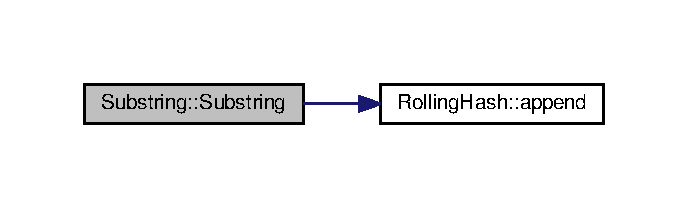
\includegraphics[width=330pt]{classSubstring_a065a95aaacde32e5b623f0a52d3ca180_cgraph}
\end{center}
\end{figure}


\hypertarget{classSubstring_ac486fd7645e645efd9c5a07b5e664b20}{\index{Substring@{Substring}!````~Substring@{$\sim$\+Substring}}
\index{````~Substring@{$\sim$\+Substring}!Substring@{Substring}}
\subsubsection[{$\sim$\+Substring}]{\setlength{\rightskip}{0pt plus 5cm}template$<$typename Type\+Of\+Content$>$ {\bf Substring}$<$ Type\+Of\+Content $>$\+::$\sim${\bf Substring} (
\begin{DoxyParamCaption}
{}
\end{DoxyParamCaption}
)\hspace{0.3cm}{\ttfamily [inline]}}}\label{classSubstring_ac486fd7645e645efd9c5a07b5e664b20}
Destrutor da classe \hyperlink{classSubstring}{Substring} 

Definition at line 88 of file Substring.\+h.



References Substring$<$ Type\+Of\+Content $>$\+::rolling\+Hash.



\subsection{Member Function Documentation}
\hypertarget{classSubstring_ae5eb3f9712352741b8bf65b2b231356c}{\index{Substring@{Substring}!append@{append}}
\index{append@{append}!Substring@{Substring}}
\subsubsection[{append}]{\setlength{\rightskip}{0pt plus 5cm}template$<$typename Type\+Of\+Content$>$ void {\bf Substring}$<$ Type\+Of\+Content $>$\+::append (
\begin{DoxyParamCaption}
{}
\end{DoxyParamCaption}
)\hspace{0.3cm}{\ttfamily [inline]}}}\label{classSubstring_ae5eb3f9712352741b8bf65b2b231356c}
Método que adiciona um novo termo a substring. Isto é feito através do ponteiro para a string que a contém. Adicionamos o termo posterior a substring. \begin{DoxySeeAlso}{See also}
\hyperlink{classRollingHash}{Rolling\+Hash} 
\end{DoxySeeAlso}
\begin{DoxyReturn}{Returns}
void 
\end{DoxyReturn}


Definition at line 100 of file Substring.\+h.



References Rolling\+Hash$<$ Type\+Of\+Content $>$\+::append(), and Rolling\+Hash$<$ Type\+Of\+Content $>$\+::end.



Referenced by R\+K\+R\+G\+S\+T$<$ Type\+Of\+Content $>$\+::fill\+Text\+Hash\+Table().



Here is the call graph for this function\+:\nopagebreak
\begin{figure}[H]
\begin{center}
\leavevmode
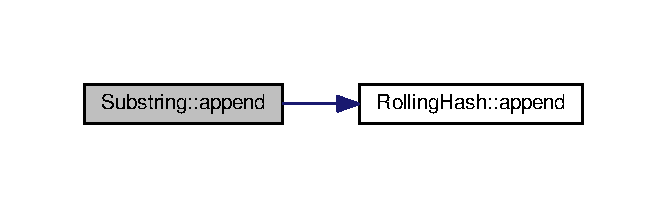
\includegraphics[width=320pt]{classSubstring_ae5eb3f9712352741b8bf65b2b231356c_cgraph}
\end{center}
\end{figure}


\hypertarget{classSubstring_a217db9ee47a8cc5db31a671606e039b5}{\index{Substring@{Substring}!print@{print}}
\index{print@{print}!Substring@{Substring}}
\subsubsection[{print}]{\setlength{\rightskip}{0pt plus 5cm}template$<$typename Type\+Of\+Content$>$ void {\bf Substring}$<$ Type\+Of\+Content $>$\+::print (
\begin{DoxyParamCaption}
{}
\end{DoxyParamCaption}
)\hspace{0.3cm}{\ttfamily [inline]}}}\label{classSubstring_a217db9ee47a8cc5db31a671606e039b5}
Imprimindo indices e valor de hash da substring \begin{DoxySeeAlso}{See also}
\hyperlink{classRollingHash}{Rolling\+Hash} 
\end{DoxySeeAlso}
\begin{DoxyReturn}{Returns}
void 
\end{DoxyReturn}


Definition at line 124 of file Substring.\+h.



References Rolling\+Hash$<$ Type\+Of\+Content $>$\+::begin, Rolling\+Hash$<$ Type\+Of\+Content $>$\+::end, and Rolling\+Hash$<$ Type\+Of\+Content $>$\+::hash\+Value.



Referenced by Hash\+Table$<$ Type\+Of\+Content $>$\+::print\+Hash\+Table().

\hypertarget{classSubstring_a618432b07f7469537bd8de5c9dccc02f}{\index{Substring@{Substring}!skip@{skip}}
\index{skip@{skip}!Substring@{Substring}}
\subsubsection[{skip}]{\setlength{\rightskip}{0pt plus 5cm}template$<$typename Type\+Of\+Content$>$ void {\bf Substring}$<$ Type\+Of\+Content $>$\+::skip (
\begin{DoxyParamCaption}
{}
\end{DoxyParamCaption}
)\hspace{0.3cm}{\ttfamily [inline]}}}\label{classSubstring_a618432b07f7469537bd8de5c9dccc02f}
Método que remove um termo da substring. \begin{DoxySeeAlso}{See also}
\hyperlink{classRollingHash}{Rolling\+Hash} 
\end{DoxySeeAlso}
\begin{DoxyReturn}{Returns}
void 
\end{DoxyReturn}


Definition at line 112 of file Substring.\+h.



References Rolling\+Hash$<$ Type\+Of\+Content $>$\+::skip().



Referenced by R\+K\+R\+G\+S\+T$<$ Type\+Of\+Content $>$\+::fill\+Text\+Hash\+Table().



Here is the call graph for this function\+:\nopagebreak
\begin{figure}[H]
\begin{center}
\leavevmode
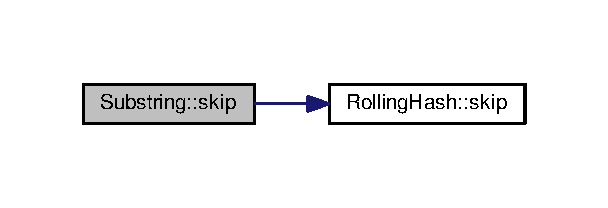
\includegraphics[width=292pt]{classSubstring_a618432b07f7469537bd8de5c9dccc02f_cgraph}
\end{center}
\end{figure}




\subsection{Member Data Documentation}
\hypertarget{classSubstring_a88e2864cc7847c7f57815de891246cfe}{\index{Substring@{Substring}!begin@{begin}}
\index{begin@{begin}!Substring@{Substring}}
\subsubsection[{begin}]{\setlength{\rightskip}{0pt plus 5cm}template$<$typename Type\+Of\+Content$>$ int {\bf Substring}$<$ Type\+Of\+Content $>$\+::begin}}\label{classSubstring_a88e2864cc7847c7f57815de891246cfe}


Índice inicial da substring na sua string de origem. 



Definition at line 52 of file Substring.\+h.



Referenced by R\+K\+R\+G\+S\+T$<$ Type\+Of\+Content $>$\+::fill\+Text\+Hash\+Table(), R\+K\+R\+G\+S\+T$<$ Type\+Of\+Content $>$\+::scan\+Pattern(), and Substring$<$ Type\+Of\+Content $>$\+::\+Substring().

\hypertarget{classSubstring_a5a223bd1f3483d1ee55f4b3997a48862}{\index{Substring@{Substring}!end@{end}}
\index{end@{end}!Substring@{Substring}}
\subsubsection[{end}]{\setlength{\rightskip}{0pt plus 5cm}template$<$typename Type\+Of\+Content$>$ int {\bf Substring}$<$ Type\+Of\+Content $>$\+::end}}\label{classSubstring_a5a223bd1f3483d1ee55f4b3997a48862}


Índice inicial da substring na sua string de origem. 



Definition at line 55 of file Substring.\+h.



Referenced by R\+K\+R\+G\+S\+T$<$ Type\+Of\+Content $>$\+::fill\+Text\+Hash\+Table(), and Substring$<$ Type\+Of\+Content $>$\+::\+Substring().

\hypertarget{classSubstring_a5965b296a10e4a5fd874913f07754451}{\index{Substring@{Substring}!next@{next}}
\index{next@{next}!Substring@{Substring}}
\subsubsection[{next}]{\setlength{\rightskip}{0pt plus 5cm}template$<$typename Type\+Of\+Content$>$ {\bf Substring}$<$Type\+Of\+Content$>$$\ast$ {\bf Substring}$<$ Type\+Of\+Content $>$\+::next}}\label{classSubstring_a5965b296a10e4a5fd874913f07754451}


Ponteiro para a próxima substring na lista. 



Definition at line 44 of file Substring.\+h.



Referenced by List\+Of\+Substrings$<$ Type\+Of\+Content $>$\+::add\+Substring(), R\+K\+R\+G\+S\+T$<$ Type\+Of\+Content $>$\+::fill\+Text\+Hash\+Table(), Hash\+Table$<$ Type\+Of\+Content $>$\+::print\+Hash\+Table(), R\+K\+R\+G\+S\+T$<$ Type\+Of\+Content $>$\+::scan\+Pattern(), and List\+Of\+Substrings$<$ Type\+Of\+Content $>$\+::$\sim$\+List\+Of\+Substrings().

\hypertarget{classSubstring_a992d0f85409426c420d243ac18d2bca5}{\index{Substring@{Substring}!previous@{previous}}
\index{previous@{previous}!Substring@{Substring}}
\subsubsection[{previous}]{\setlength{\rightskip}{0pt plus 5cm}template$<$typename Type\+Of\+Content$>$ {\bf Substring}$<$Type\+Of\+Content$>$$\ast$ {\bf Substring}$<$ Type\+Of\+Content $>$\+::previous}}\label{classSubstring_a992d0f85409426c420d243ac18d2bca5}


Ponteiro para a substring anterior na lista. 



Definition at line 46 of file Substring.\+h.



Referenced by List\+Of\+Substrings$<$ Type\+Of\+Content $>$\+::add\+Substring(), and R\+K\+R\+G\+S\+T$<$ Type\+Of\+Content $>$\+::fill\+Text\+Hash\+Table().

\hypertarget{classSubstring_a84e0e55a0ecbd5f74d25441df0edc68e}{\index{Substring@{Substring}!rolling\+Hash@{rolling\+Hash}}
\index{rolling\+Hash@{rolling\+Hash}!Substring@{Substring}}
\subsubsection[{rolling\+Hash}]{\setlength{\rightskip}{0pt plus 5cm}template$<$typename Type\+Of\+Content$>$ {\bf Rolling\+Hash}$<$Type\+Of\+Content$>$$\ast$ {\bf Substring}$<$ Type\+Of\+Content $>$\+::rolling\+Hash}}\label{classSubstring_a84e0e55a0ecbd5f74d25441df0edc68e}


ponteiro para a hash relativa ao seu conteúdo 



Definition at line 49 of file Substring.\+h.



Referenced by Hash\+Table$<$ Type\+Of\+Content $>$\+::add\+Hash(), R\+K\+R\+G\+S\+T$<$ Type\+Of\+Content $>$\+::fill\+Text\+Hash\+Table(), R\+K\+R\+G\+S\+T$<$ Type\+Of\+Content $>$\+::scan\+Pattern(), and Substring$<$ Type\+Of\+Content $>$\+::$\sim$\+Substring().

\hypertarget{classSubstring_a8d1fd97efa348288f4b39bea36a8e879}{\index{Substring@{Substring}!string@{string}}
\index{string@{string}!Substring@{Substring}}
\subsubsection[{string}]{\setlength{\rightskip}{0pt plus 5cm}template$<$typename Type\+Of\+Content$>$ {\bf Letter}$<$Type\+Of\+Content$>$$\ast$ {\bf Substring}$<$ Type\+Of\+Content $>$\+::{\bf string}}}\label{classSubstring_a8d1fd97efa348288f4b39bea36a8e879}


Ponteiro para a string que a contém. 



Definition at line 42 of file Substring.\+h.



Referenced by R\+K\+R\+G\+S\+T$<$ Type\+Of\+Content $>$\+::fill\+Text\+Hash\+Table(), R\+K\+R\+G\+S\+T$<$ Type\+Of\+Content $>$\+::scan\+Pattern(), and Substring$<$ Type\+Of\+Content $>$\+::\+Substring().



The documentation for this class was generated from the following file\+:\begin{DoxyCompactItemize}
\item 
\hyperlink{Substring_8h}{Substring.\+h}\end{DoxyCompactItemize}

\hypertarget{classTile}{\section{Tile Class Reference}
\label{classTile}\index{Tile@{Tile}}
}


{\ttfamily \#include $<$Tile.\+h$>$}



Collaboration diagram for Tile\+:\nopagebreak
\begin{figure}[H]
\begin{center}
\leavevmode
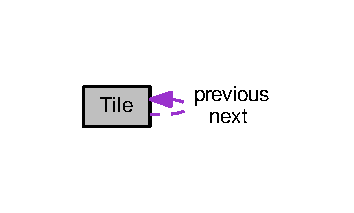
\includegraphics[width=170pt]{classTile__coll__graph}
\end{center}
\end{figure}
\subsection*{Public Member Functions}
\begin{DoxyCompactItemize}
\item 
\hyperlink{classTile_a4f59f006f6a5e1cd5cc5b269a29d067b}{Tile} (int \hyperlink{classTile_abf2eb9ed61ada2b1a35386e5f20bd350}{begin}, int \hyperlink{classTile_a39ee840ddb65bf9ad1fb12667e92993c}{end})
\end{DoxyCompactItemize}
\subsection*{Public Attributes}
\begin{DoxyCompactItemize}
\item 
\hyperlink{classTile}{Tile} $\ast$ \hyperlink{classTile_a3c9f5e6070368625c8bfc8b9d30282ca}{next}
\begin{DoxyCompactList}\small\item\em ponteiro para o próximo objeto da classe \hyperlink{classTile}{Tile} contido na mesma lista que este \end{DoxyCompactList}\item 
\hyperlink{classTile}{Tile} $\ast$ \hyperlink{classTile_ac5e5e631733d14196575bd39d5df8923}{previous}
\begin{DoxyCompactList}\small\item\em ponteiro para o prévio objeto da classe \hyperlink{classTile}{Tile} contido na mesma lista que este \end{DoxyCompactList}\item 
int \hyperlink{classTile_abf2eb9ed61ada2b1a35386e5f20bd350}{begin}
\begin{DoxyCompactList}\small\item\em Índice para a letra inicial deste \hyperlink{classTile}{Tile} na string. \end{DoxyCompactList}\item 
int \hyperlink{classTile_a39ee840ddb65bf9ad1fb12667e92993c}{end}
\begin{DoxyCompactList}\small\item\em Índice para a letra final deste \hyperlink{classTile}{Tile} na string. \end{DoxyCompactList}\end{DoxyCompactItemize}


\subsection{Detailed Description}
Classe referente a uma \hyperlink{classTile}{Tile}. 

Definition at line 31 of file Tile.\+h.



\subsection{Constructor \& Destructor Documentation}
\hypertarget{classTile_a4f59f006f6a5e1cd5cc5b269a29d067b}{\index{Tile@{Tile}!Tile@{Tile}}
\index{Tile@{Tile}!Tile@{Tile}}
\subsubsection[{Tile}]{\setlength{\rightskip}{0pt plus 5cm}Tile\+::\+Tile (
\begin{DoxyParamCaption}
\item[{int}]{begin, }
\item[{int}]{end}
\end{DoxyParamCaption}
)\hspace{0.3cm}{\ttfamily [inline]}}}\label{classTile_a4f59f006f6a5e1cd5cc5b269a29d067b}
Construtor de um objeto da classe \hyperlink{classTile}{Tile} 
\begin{DoxyParams}{Parameters}
{\em begin} & Índice da posição inicial do \hyperlink{classTile}{Tile} na string \\
\hline
{\em end} & Índice da posição final do \hyperlink{classTile}{Tile} na string \\
\hline
\end{DoxyParams}


Definition at line 50 of file Tile.\+h.



References begin, and end.



\subsection{Member Data Documentation}
\hypertarget{classTile_abf2eb9ed61ada2b1a35386e5f20bd350}{\index{Tile@{Tile}!begin@{begin}}
\index{begin@{begin}!Tile@{Tile}}
\subsubsection[{begin}]{\setlength{\rightskip}{0pt plus 5cm}int Tile\+::begin}}\label{classTile_abf2eb9ed61ada2b1a35386e5f20bd350}


Índice para a letra inicial deste \hyperlink{classTile}{Tile} na string. 



Definition at line 40 of file Tile.\+h.



Referenced by R\+K\+R\+G\+S\+T$<$ Type\+Of\+Content $>$\+::fill\+Text\+Hash\+Table(), R\+K\+R\+G\+S\+T$<$ Type\+Of\+Content $>$\+::find\+Pattern\+Substring(), List\+Of\+Tiles\+::print(), List\+Of\+Tiles\+::remove\+Tile(), and Tile().

\hypertarget{classTile_a39ee840ddb65bf9ad1fb12667e92993c}{\index{Tile@{Tile}!end@{end}}
\index{end@{end}!Tile@{Tile}}
\subsubsection[{end}]{\setlength{\rightskip}{0pt plus 5cm}int Tile\+::end}}\label{classTile_a39ee840ddb65bf9ad1fb12667e92993c}


Índice para a letra final deste \hyperlink{classTile}{Tile} na string. 



Definition at line 43 of file Tile.\+h.



Referenced by R\+K\+R\+G\+S\+T$<$ Type\+Of\+Content $>$\+::fill\+Text\+Hash\+Table(), R\+K\+R\+G\+S\+T$<$ Type\+Of\+Content $>$\+::find\+Pattern\+Substring(), List\+Of\+Tiles\+::print(), List\+Of\+Tiles\+::remove\+Tile(), and Tile().

\hypertarget{classTile_a3c9f5e6070368625c8bfc8b9d30282ca}{\index{Tile@{Tile}!next@{next}}
\index{next@{next}!Tile@{Tile}}
\subsubsection[{next}]{\setlength{\rightskip}{0pt plus 5cm}{\bf Tile}$\ast$ Tile\+::next}}\label{classTile_a3c9f5e6070368625c8bfc8b9d30282ca}


ponteiro para o próximo objeto da classe \hyperlink{classTile}{Tile} contido na mesma lista que este 



Definition at line 35 of file Tile.\+h.



Referenced by List\+Of\+Tiles\+::add\+Tile(), R\+K\+R\+G\+S\+T$<$ Type\+Of\+Content $>$\+::fill\+Text\+Hash\+Table(), R\+K\+R\+G\+S\+T$<$ Type\+Of\+Content $>$\+::find\+Pattern\+Substring(), List\+Of\+Tiles\+::print(), List\+Of\+Tiles\+::remove\+Tile(), and List\+Of\+Tiles\+::$\sim$\+List\+Of\+Tiles().

\hypertarget{classTile_ac5e5e631733d14196575bd39d5df8923}{\index{Tile@{Tile}!previous@{previous}}
\index{previous@{previous}!Tile@{Tile}}
\subsubsection[{previous}]{\setlength{\rightskip}{0pt plus 5cm}{\bf Tile}$\ast$ Tile\+::previous}}\label{classTile_ac5e5e631733d14196575bd39d5df8923}


ponteiro para o prévio objeto da classe \hyperlink{classTile}{Tile} contido na mesma lista que este 



Definition at line 37 of file Tile.\+h.



Referenced by List\+Of\+Tiles\+::add\+Tile(), and List\+Of\+Tiles\+::remove\+Tile().



The documentation for this class was generated from the following file\+:\begin{DoxyCompactItemize}
\item 
\hyperlink{Tile_8h}{Tile.\+h}\end{DoxyCompactItemize}

\chapter{File Documentation}
\hypertarget{Box_8h}{\section{Box.\+h File Reference}
\label{Box_8h}\index{Box.\+h@{Box.\+h}}
}
{\ttfamily \#include \char`\"{}Letter.\+h\char`\"{}}\\*
{\ttfamily \#include $<$stdio.\+h$>$}\\*
Include dependency graph for Box.\+h\+:\nopagebreak
\begin{figure}[H]
\begin{center}
\leavevmode
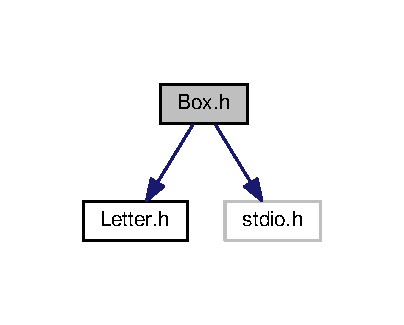
\includegraphics[width=194pt]{Box_8h__incl}
\end{center}
\end{figure}
This graph shows which files directly or indirectly include this file\+:\nopagebreak
\begin{figure}[H]
\begin{center}
\leavevmode
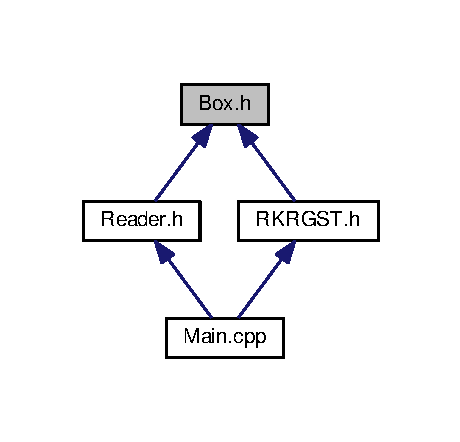
\includegraphics[width=221pt]{Box_8h__dep__incl}
\end{center}
\end{figure}
\subsection*{Classes}
\begin{DoxyCompactItemize}
\item 
class \hyperlink{classBox}{Box$<$ Type\+Of\+Content $>$}
\end{DoxyCompactItemize}

\hypertarget{HashTable_8h}{\section{Hash\+Table.\+h File Reference}
\label{HashTable_8h}\index{Hash\+Table.\+h@{Hash\+Table.\+h}}
}
{\ttfamily \#include \char`\"{}List\+Of\+Substrings.\+h\char`\"{}}\\*
{\ttfamily \#include $<$iostream$>$}\\*
Include dependency graph for Hash\+Table.\+h\+:\nopagebreak
\begin{figure}[H]
\begin{center}
\leavevmode
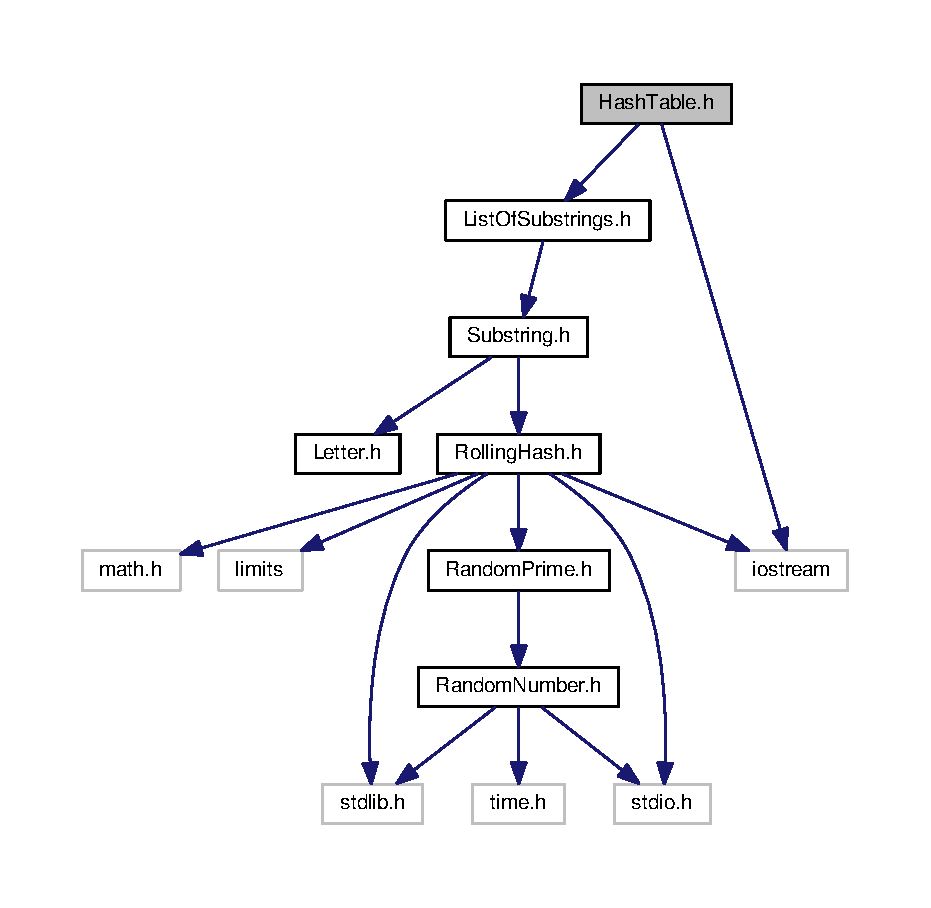
\includegraphics[width=350pt]{HashTable_8h__incl}
\end{center}
\end{figure}
This graph shows which files directly or indirectly include this file\+:\nopagebreak
\begin{figure}[H]
\begin{center}
\leavevmode
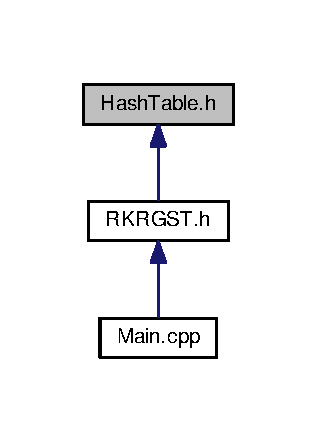
\includegraphics[width=152pt]{HashTable_8h__dep__incl}
\end{center}
\end{figure}
\subsection*{Classes}
\begin{DoxyCompactItemize}
\item 
class \hyperlink{classHashTable}{Hash\+Table$<$ Type\+Of\+Content $>$}
\end{DoxyCompactItemize}

\hypertarget{Letter_8h}{\section{Letter.\+h File Reference}
\label{Letter_8h}\index{Letter.\+h@{Letter.\+h}}
}
This graph shows which files directly or indirectly include this file\+:\nopagebreak
\begin{figure}[H]
\begin{center}
\leavevmode
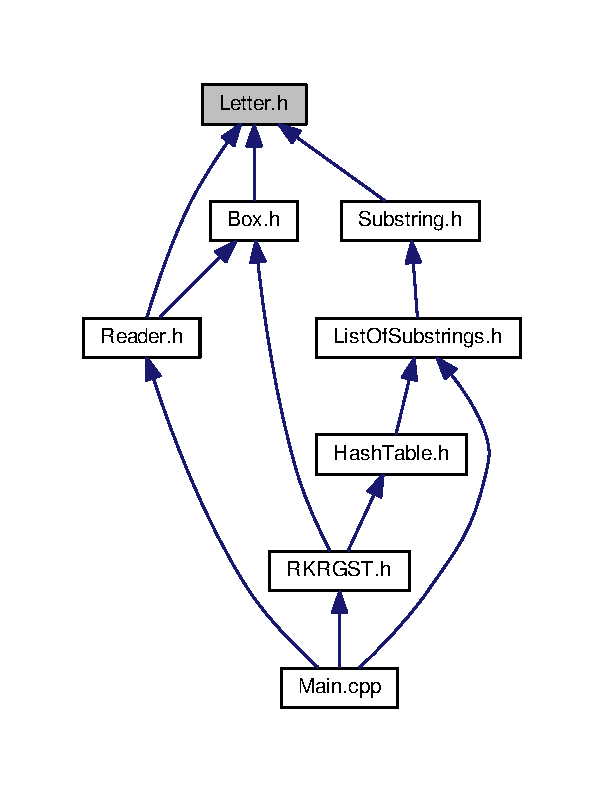
\includegraphics[width=289pt]{Letter_8h__dep__incl}
\end{center}
\end{figure}
\subsection*{Classes}
\begin{DoxyCompactItemize}
\item 
class \hyperlink{classLetter}{Letter$<$ Type\+Of\+Content $>$}
\end{DoxyCompactItemize}

\hypertarget{ListOfMatches_8cpp}{\section{List\+Of\+Matches.\+cpp File Reference}
\label{ListOfMatches_8cpp}\index{List\+Of\+Matches.\+cpp@{List\+Of\+Matches.\+cpp}}
}
{\ttfamily \#include \char`\"{}List\+Of\+Matches.\+h\char`\"{}}\\*
Include dependency graph for List\+Of\+Matches.\+cpp\+:\nopagebreak
\begin{figure}[H]
\begin{center}
\leavevmode
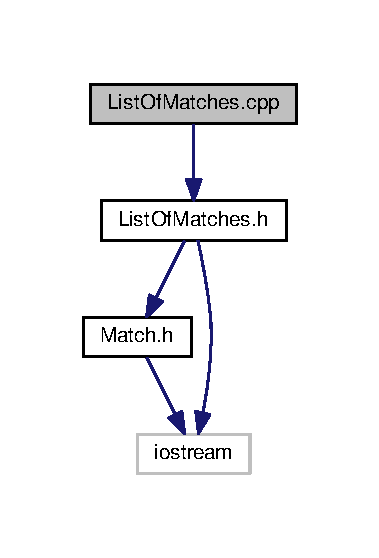
\includegraphics[width=182pt]{ListOfMatches_8cpp__incl}
\end{center}
\end{figure}

\hypertarget{ListOfMatches_8h}{\section{List\+Of\+Matches.\+h File Reference}
\label{ListOfMatches_8h}\index{List\+Of\+Matches.\+h@{List\+Of\+Matches.\+h}}
}
{\ttfamily \#include \char`\"{}Match.\+h\char`\"{}}\\*
{\ttfamily \#include $<$iostream$>$}\\*
Include dependency graph for List\+Of\+Matches.\+h\+:\nopagebreak
\begin{figure}[H]
\begin{center}
\leavevmode
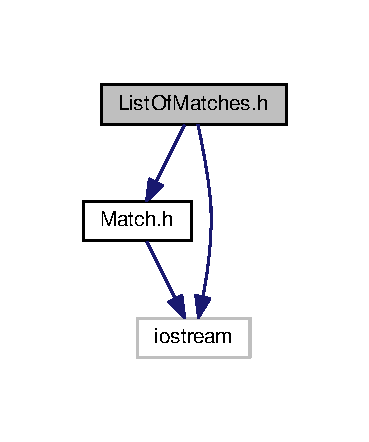
\includegraphics[width=177pt]{ListOfMatches_8h__incl}
\end{center}
\end{figure}
This graph shows which files directly or indirectly include this file\+:\nopagebreak
\begin{figure}[H]
\begin{center}
\leavevmode
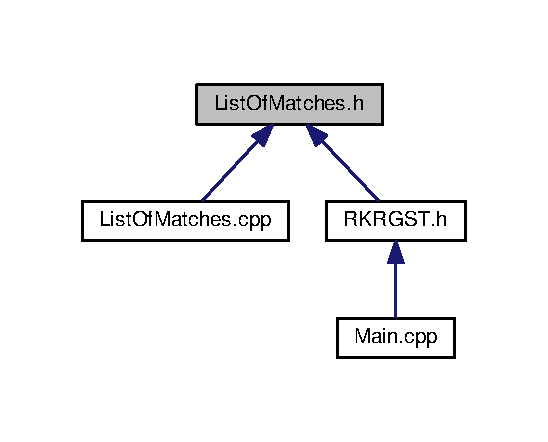
\includegraphics[width=263pt]{ListOfMatches_8h__dep__incl}
\end{center}
\end{figure}
\subsection*{Classes}
\begin{DoxyCompactItemize}
\item 
class \hyperlink{classListOfMatches}{List\+Of\+Matches}
\end{DoxyCompactItemize}

\hypertarget{ListOfSubstrings_8h}{\section{List\+Of\+Substrings.\+h File Reference}
\label{ListOfSubstrings_8h}\index{List\+Of\+Substrings.\+h@{List\+Of\+Substrings.\+h}}
}
{\ttfamily \#include \char`\"{}Substring.\+h\char`\"{}}\\*
Include dependency graph for List\+Of\+Substrings.\+h\+:\nopagebreak
\begin{figure}[H]
\begin{center}
\leavevmode
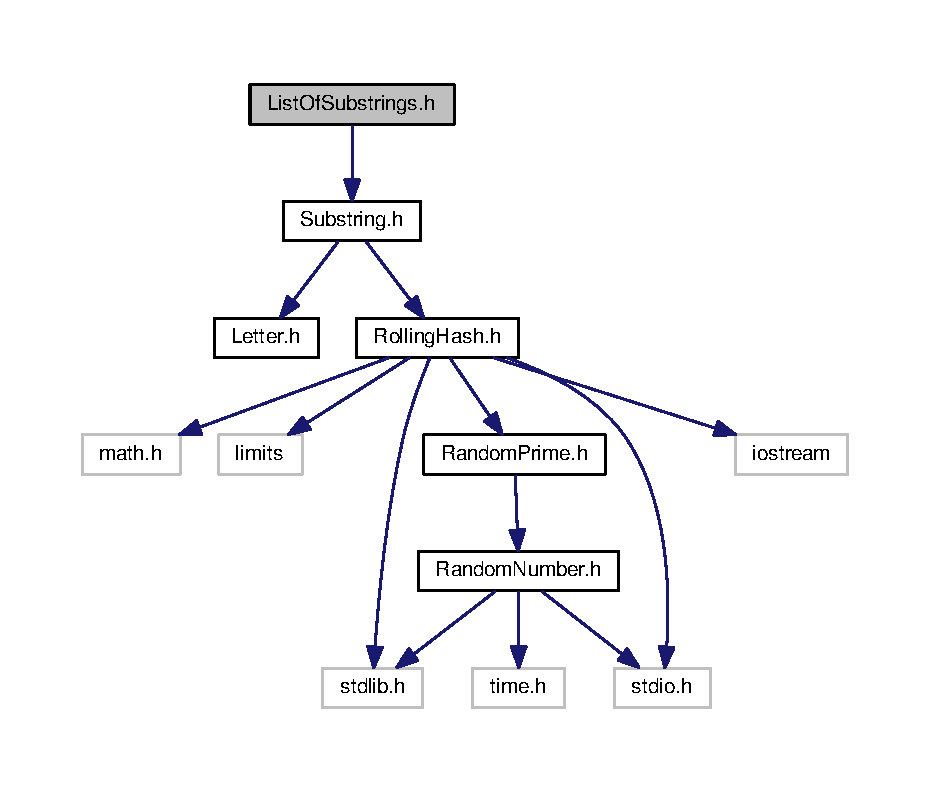
\includegraphics[width=350pt]{ListOfSubstrings_8h__incl}
\end{center}
\end{figure}
This graph shows which files directly or indirectly include this file\+:\nopagebreak
\begin{figure}[H]
\begin{center}
\leavevmode
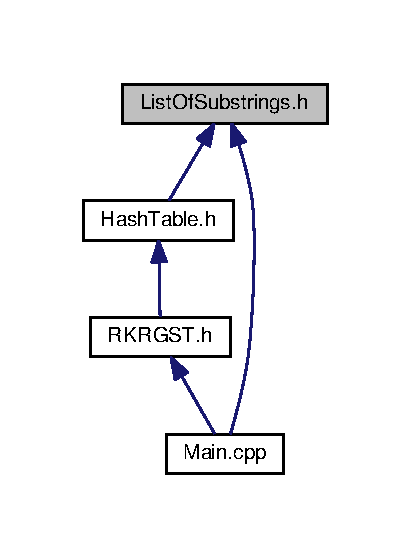
\includegraphics[width=196pt]{ListOfSubstrings_8h__dep__incl}
\end{center}
\end{figure}
\subsection*{Classes}
\begin{DoxyCompactItemize}
\item 
class \hyperlink{classListOfSubstrings}{List\+Of\+Substrings$<$ Type\+Of\+Content $>$}
\end{DoxyCompactItemize}

\hypertarget{ListOfTiles_8h}{\section{List\+Of\+Tiles.\+h File Reference}
\label{ListOfTiles_8h}\index{List\+Of\+Tiles.\+h@{List\+Of\+Tiles.\+h}}
}
{\ttfamily \#include \char`\"{}Tile.\+h\char`\"{}}\\*
{\ttfamily \#include $<$stdio.\+h$>$}\\*
Include dependency graph for List\+Of\+Tiles.\+h\+:\nopagebreak
\begin{figure}[H]
\begin{center}
\leavevmode
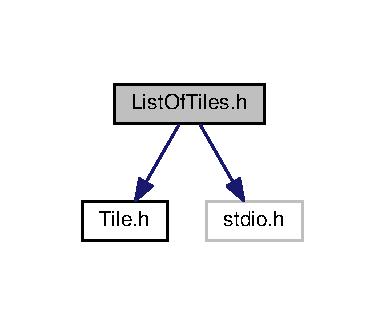
\includegraphics[width=185pt]{ListOfTiles_8h__incl}
\end{center}
\end{figure}
This graph shows which files directly or indirectly include this file\+:\nopagebreak
\begin{figure}[H]
\begin{center}
\leavevmode
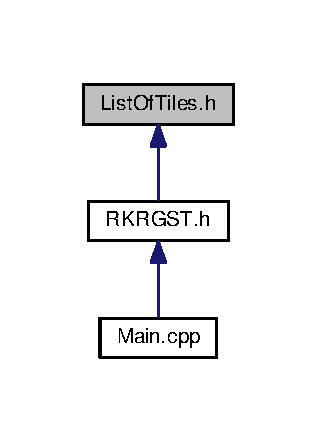
\includegraphics[width=152pt]{ListOfTiles_8h__dep__incl}
\end{center}
\end{figure}
\subsection*{Classes}
\begin{DoxyCompactItemize}
\item 
class \hyperlink{classListOfTiles}{List\+Of\+Tiles}
\end{DoxyCompactItemize}

\hypertarget{Main_8cpp}{\section{Main.\+cpp File Reference}
\label{Main_8cpp}\index{Main.\+cpp@{Main.\+cpp}}
}
{\ttfamily \#include \char`\"{}List\+Of\+Substrings.\+h\char`\"{}}\\*
{\ttfamily \#include \char`\"{}Reader.\+h\char`\"{}}\\*
{\ttfamily \#include \char`\"{}R\+K\+R\+G\+S\+T.\+h\char`\"{}}\\*
{\ttfamily \#include $<$iomanip$>$}\\*
{\ttfamily \#include $<$sys/time.\+h$>$}\\*
Include dependency graph for Main.\+cpp\+:\nopagebreak
\begin{figure}[H]
\begin{center}
\leavevmode
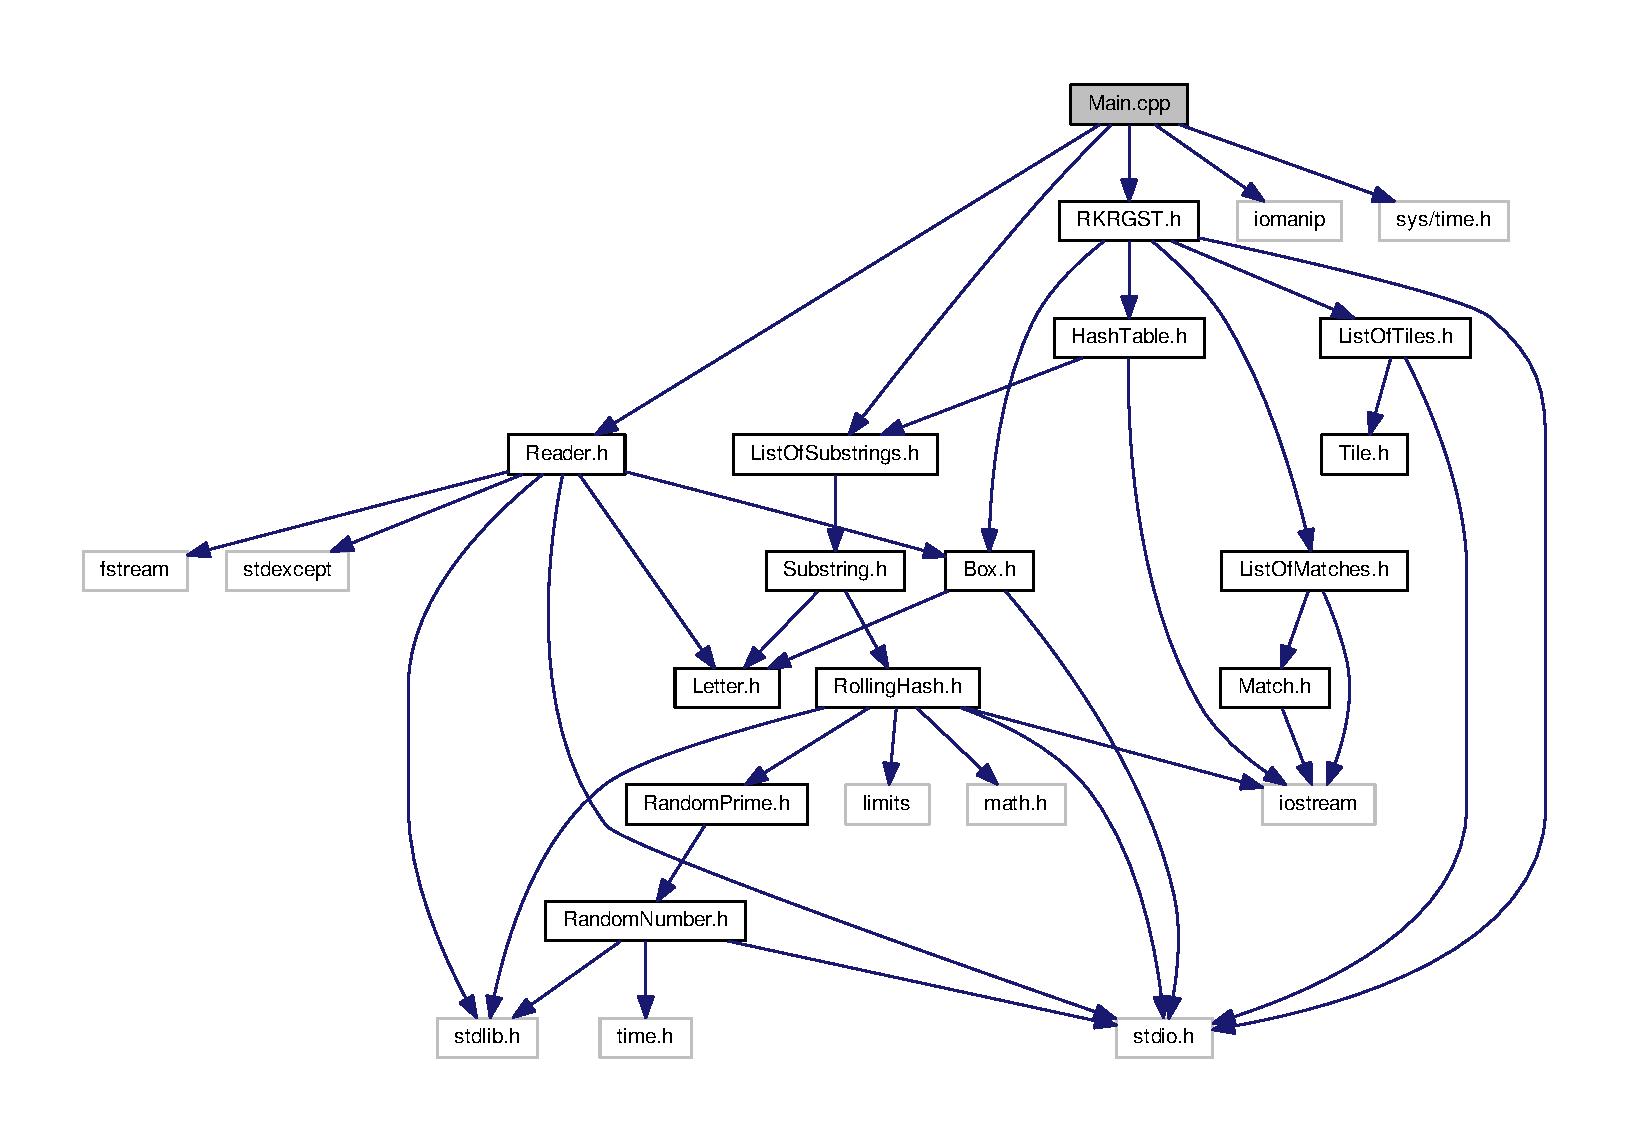
\includegraphics[width=350pt]{Main_8cpp__incl}
\end{center}
\end{figure}
\subsection*{Macros}
\begin{DoxyCompactItemize}
\item 
\#define \hyperlink{Main_8cpp_a79bcfb6bde984f42d1124b068a509af7}{B\+A\+S\+E}~2
\end{DoxyCompactItemize}
\subsection*{Typedefs}
\begin{DoxyCompactItemize}
\item 
typedef char $\ast$ \hyperlink{Main_8cpp_a4505c08c065b48840a30eedd9845cce2}{string}
\end{DoxyCompactItemize}
\subsection*{Functions}
\begin{DoxyCompactItemize}
\item 
double \hyperlink{Main_8cpp_a4437edd7fd2832790c13ba3179bcc64d}{get\+Time} ()
\item 
int \hyperlink{Main_8cpp_a3c04138a5bfe5d72780bb7e82a18e627}{main} (int argc, char $\ast$$\ast$argv)
\end{DoxyCompactItemize}


\subsection{Macro Definition Documentation}
\hypertarget{Main_8cpp_a79bcfb6bde984f42d1124b068a509af7}{\index{Main.\+cpp@{Main.\+cpp}!B\+A\+S\+E@{B\+A\+S\+E}}
\index{B\+A\+S\+E@{B\+A\+S\+E}!Main.\+cpp@{Main.\+cpp}}
\subsubsection[{B\+A\+S\+E}]{\setlength{\rightskip}{0pt plus 5cm}\#define B\+A\+S\+E~2}}\label{Main_8cpp_a79bcfb6bde984f42d1124b068a509af7}


Definition at line 35 of file Main.\+cpp.



Referenced by main().



\subsection{Typedef Documentation}
\hypertarget{Main_8cpp_a4505c08c065b48840a30eedd9845cce2}{\index{Main.\+cpp@{Main.\+cpp}!string@{string}}
\index{string@{string}!Main.\+cpp@{Main.\+cpp}}
\subsubsection[{string}]{\setlength{\rightskip}{0pt plus 5cm}typedef char$\ast$ {\bf string}}}\label{Main_8cpp_a4505c08c065b48840a30eedd9845cce2}


Definition at line 38 of file Main.\+cpp.



\subsection{Function Documentation}
\hypertarget{Main_8cpp_a4437edd7fd2832790c13ba3179bcc64d}{\index{Main.\+cpp@{Main.\+cpp}!get\+Time@{get\+Time}}
\index{get\+Time@{get\+Time}!Main.\+cpp@{Main.\+cpp}}
\subsubsection[{get\+Time}]{\setlength{\rightskip}{0pt plus 5cm}double get\+Time (
\begin{DoxyParamCaption}
{}
\end{DoxyParamCaption}
)}}\label{Main_8cpp_a4437edd7fd2832790c13ba3179bcc64d}


Definition at line 50 of file Main.\+cpp.



Referenced by main().

\hypertarget{Main_8cpp_a3c04138a5bfe5d72780bb7e82a18e627}{\index{Main.\+cpp@{Main.\+cpp}!main@{main}}
\index{main@{main}!Main.\+cpp@{Main.\+cpp}}
\subsubsection[{main}]{\setlength{\rightskip}{0pt plus 5cm}int main (
\begin{DoxyParamCaption}
\item[{int}]{argc, }
\item[{char $\ast$$\ast$}]{argv}
\end{DoxyParamCaption}
)}}\label{Main_8cpp_a3c04138a5bfe5d72780bb7e82a18e627}


Definition at line 58 of file Main.\+cpp.



References B\+A\+S\+E, R\+K\+R\+G\+S\+T$<$ Type\+Of\+Content $>$\+::execute(), Reader$<$ Type\+Of\+Content $>$\+::files\+To\+Box(), get\+Time(), Match\+::length, R\+K\+R\+G\+S\+T$<$ Type\+Of\+Content $>$\+::length\+Of\+Tokens\+Tiled, R\+K\+R\+G\+S\+T$<$ Type\+Of\+Content $>$\+::list\+Of\+Final\+Tiles, List\+Of\+Matches\+::number\+Of\+Matches, Match\+::pattern\+Index, Match\+::print(), List\+Of\+Matches\+::remove(), and Match\+::text\+Index.



Here is the call graph for this function\+:\nopagebreak
\begin{figure}[H]
\begin{center}
\leavevmode
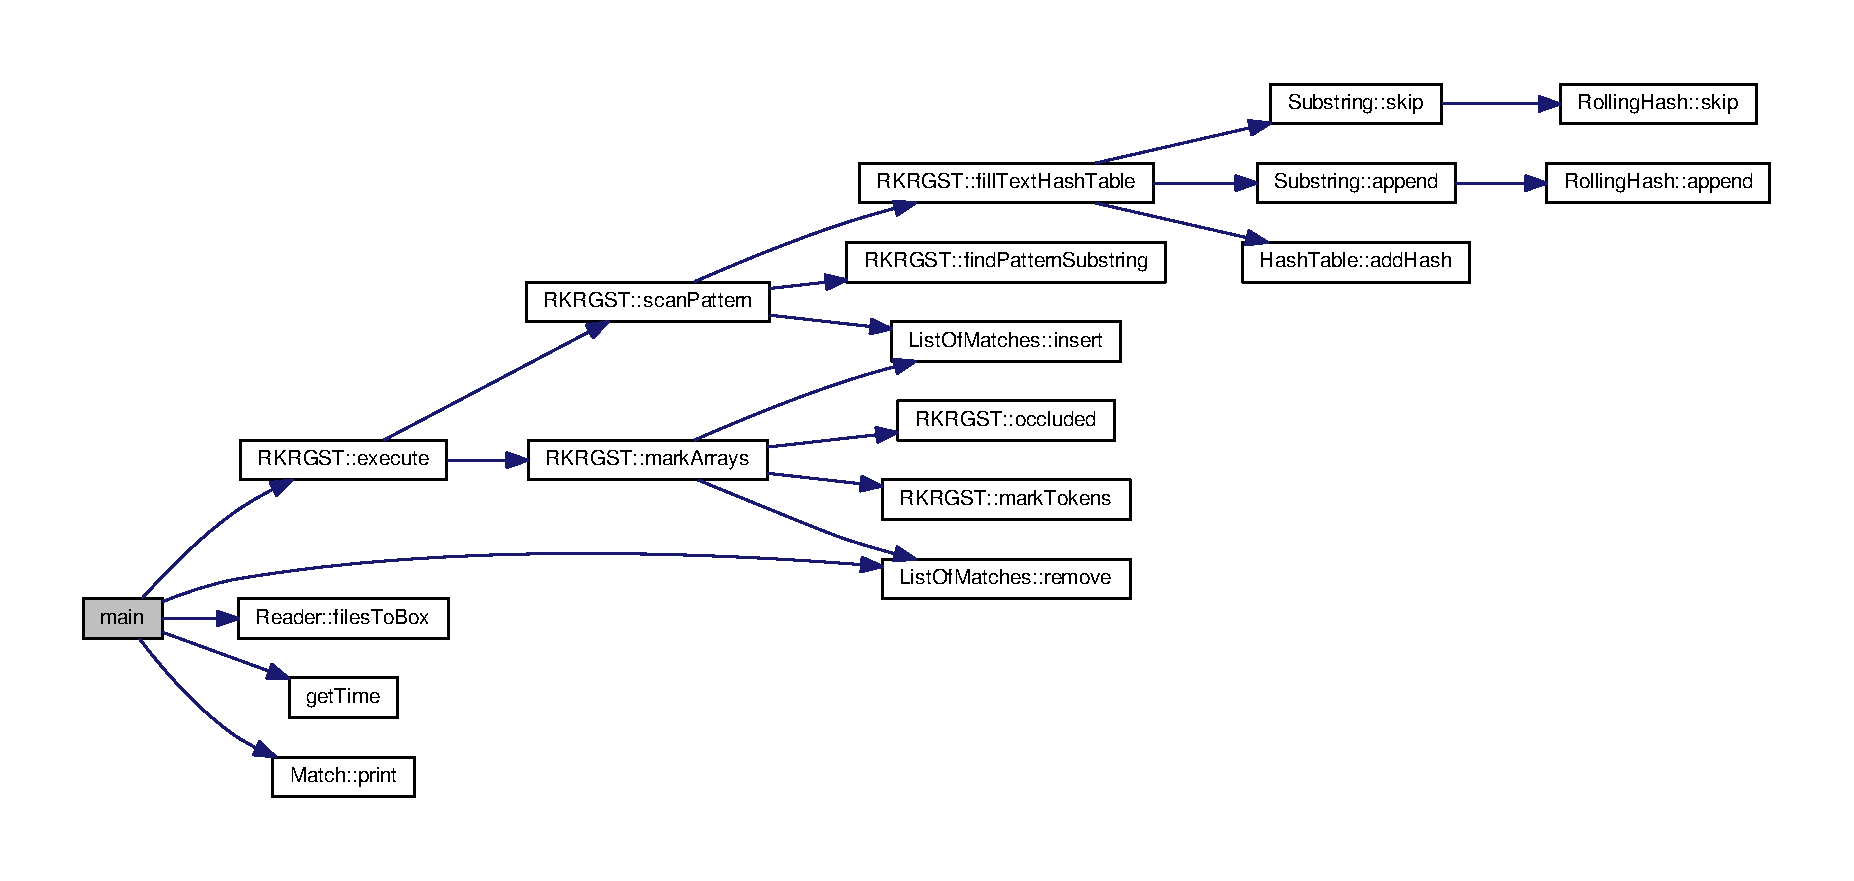
\includegraphics[width=350pt]{Main_8cpp_a3c04138a5bfe5d72780bb7e82a18e627_cgraph}
\end{center}
\end{figure}



\hypertarget{Match_8h}{\section{Match.\+h File Reference}
\label{Match_8h}\index{Match.\+h@{Match.\+h}}
}
{\ttfamily \#include $<$iostream$>$}\\*
Include dependency graph for Match.\+h\+:\nopagebreak
\begin{figure}[H]
\begin{center}
\leavevmode
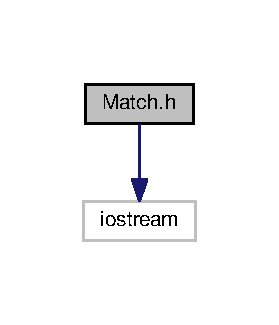
\includegraphics[width=134pt]{Match_8h__incl}
\end{center}
\end{figure}
This graph shows which files directly or indirectly include this file\+:\nopagebreak
\begin{figure}[H]
\begin{center}
\leavevmode
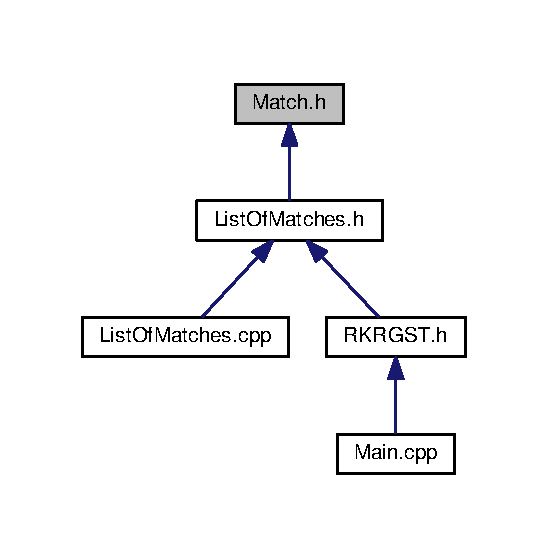
\includegraphics[width=263pt]{Match_8h__dep__incl}
\end{center}
\end{figure}
\subsection*{Classes}
\begin{DoxyCompactItemize}
\item 
class \hyperlink{classMatch}{Match}
\end{DoxyCompactItemize}

\hypertarget{RandomNumber_8h}{\section{Random\+Number.\+h File Reference}
\label{RandomNumber_8h}\index{Random\+Number.\+h@{Random\+Number.\+h}}
}
{\ttfamily \#include $<$stdlib.\+h$>$}\\*
{\ttfamily \#include $<$time.\+h$>$}\\*
{\ttfamily \#include $<$stdio.\+h$>$}\\*
Include dependency graph for Random\+Number.\+h\+:\nopagebreak
\begin{figure}[H]
\begin{center}
\leavevmode
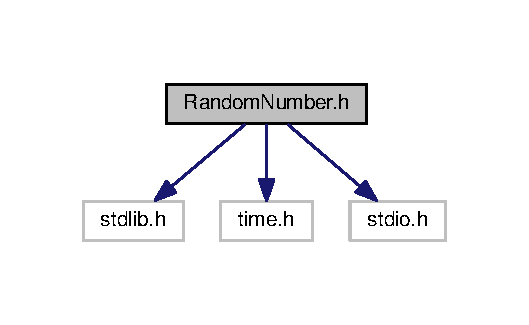
\includegraphics[width=254pt]{RandomNumber_8h__incl}
\end{center}
\end{figure}
This graph shows which files directly or indirectly include this file\+:\nopagebreak
\begin{figure}[H]
\begin{center}
\leavevmode
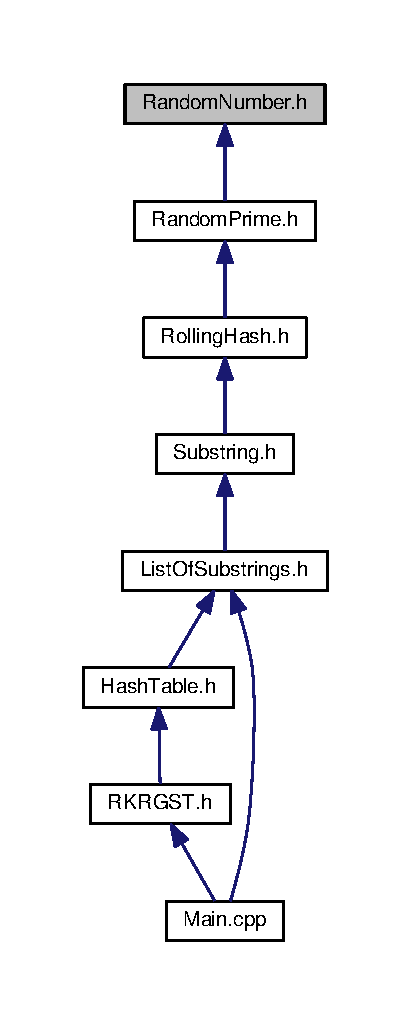
\includegraphics[width=196pt]{RandomNumber_8h__dep__incl}
\end{center}
\end{figure}
\subsection*{Classes}
\begin{DoxyCompactItemize}
\item 
class \hyperlink{classRandomNumber}{Random\+Number}
\end{DoxyCompactItemize}

\hypertarget{RandomPrime_8h}{\section{Random\+Prime.\+h File Reference}
\label{RandomPrime_8h}\index{Random\+Prime.\+h@{Random\+Prime.\+h}}
}
{\ttfamily \#include \char`\"{}Random\+Number.\+h\char`\"{}}\\*
Include dependency graph for Random\+Prime.\+h\+:\nopagebreak
\begin{figure}[H]
\begin{center}
\leavevmode
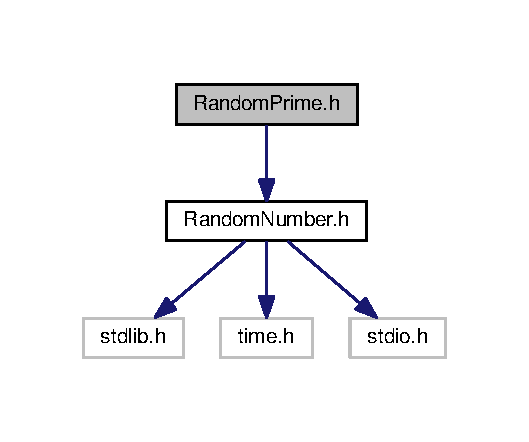
\includegraphics[width=254pt]{RandomPrime_8h__incl}
\end{center}
\end{figure}
This graph shows which files directly or indirectly include this file\+:\nopagebreak
\begin{figure}[H]
\begin{center}
\leavevmode
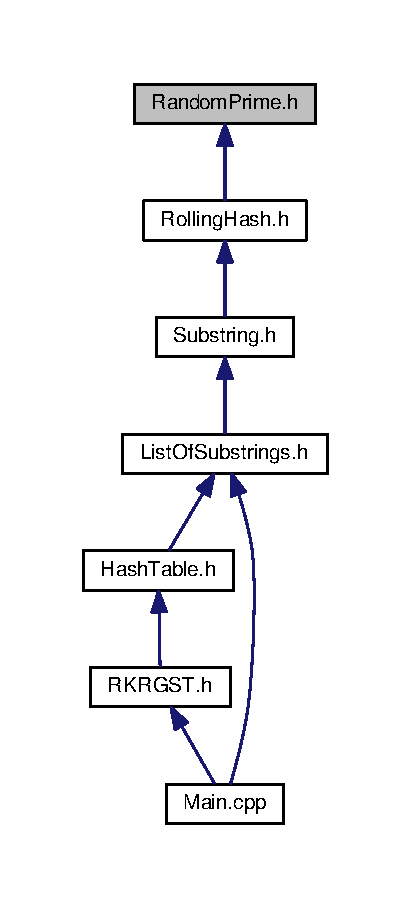
\includegraphics[width=196pt]{RandomPrime_8h__dep__incl}
\end{center}
\end{figure}
\subsection*{Classes}
\begin{DoxyCompactItemize}
\item 
class \hyperlink{classRandomPrime}{Random\+Prime}
\end{DoxyCompactItemize}

\hypertarget{Reader_8h}{\section{Reader.\+h File Reference}
\label{Reader_8h}\index{Reader.\+h@{Reader.\+h}}
}
{\ttfamily \#include \char`\"{}Letter.\+h\char`\"{}}\\*
{\ttfamily \#include \char`\"{}Box.\+h\char`\"{}}\\*
{\ttfamily \#include $<$stdio.\+h$>$}\\*
{\ttfamily \#include $<$stdlib.\+h$>$}\\*
{\ttfamily \#include $<$fstream$>$}\\*
{\ttfamily \#include $<$stdexcept$>$}\\*
Include dependency graph for Reader.\+h\+:\nopagebreak
\begin{figure}[H]
\begin{center}
\leavevmode
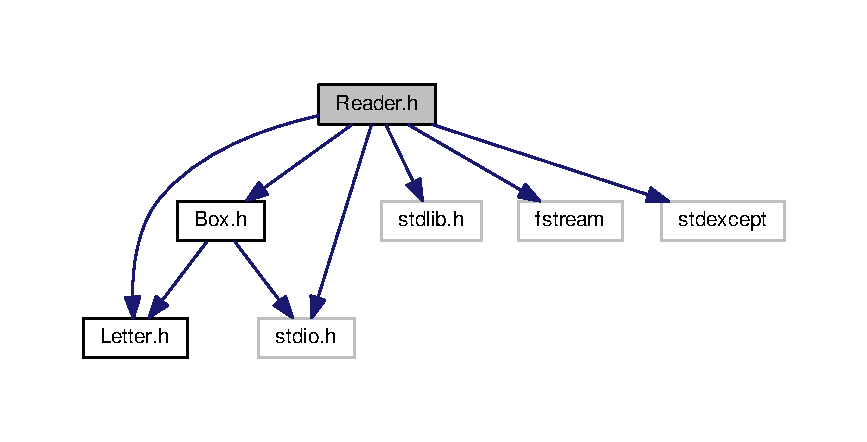
\includegraphics[width=350pt]{Reader_8h__incl}
\end{center}
\end{figure}
This graph shows which files directly or indirectly include this file\+:\nopagebreak
\begin{figure}[H]
\begin{center}
\leavevmode
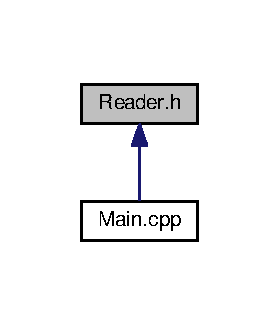
\includegraphics[width=134pt]{Reader_8h__dep__incl}
\end{center}
\end{figure}
\subsection*{Classes}
\begin{DoxyCompactItemize}
\item 
class \hyperlink{classReader}{Reader$<$ Type\+Of\+Content $>$}
\end{DoxyCompactItemize}
\subsection*{Typedefs}
\begin{DoxyCompactItemize}
\item 
typedef char $\ast$ \hyperlink{Reader_8h_a4505c08c065b48840a30eedd9845cce2}{string}
\end{DoxyCompactItemize}


\subsection{Typedef Documentation}
\hypertarget{Reader_8h_a4505c08c065b48840a30eedd9845cce2}{\index{Reader.\+h@{Reader.\+h}!string@{string}}
\index{string@{string}!Reader.\+h@{Reader.\+h}}
\subsubsection[{string}]{\setlength{\rightskip}{0pt plus 5cm}typedef char$\ast$ {\bf string}}}\label{Reader_8h_a4505c08c065b48840a30eedd9845cce2}


Definition at line 37 of file Reader.\+h.


\hypertarget{RKRGST_8h}{\section{R\+K\+R\+G\+S\+T.\+h File Reference}
\label{RKRGST_8h}\index{R\+K\+R\+G\+S\+T.\+h@{R\+K\+R\+G\+S\+T.\+h}}
}
{\ttfamily \#include \char`\"{}Box.\+h\char`\"{}}\\*
{\ttfamily \#include \char`\"{}List\+Of\+Tiles.\+h\char`\"{}}\\*
{\ttfamily \#include \char`\"{}Hash\+Table.\+h\char`\"{}}\\*
{\ttfamily \#include \char`\"{}List\+Of\+Matches.\+h\char`\"{}}\\*
{\ttfamily \#include $<$stdio.\+h$>$}\\*
Include dependency graph for R\+K\+R\+G\+S\+T.\+h\+:\nopagebreak
\begin{figure}[H]
\begin{center}
\leavevmode
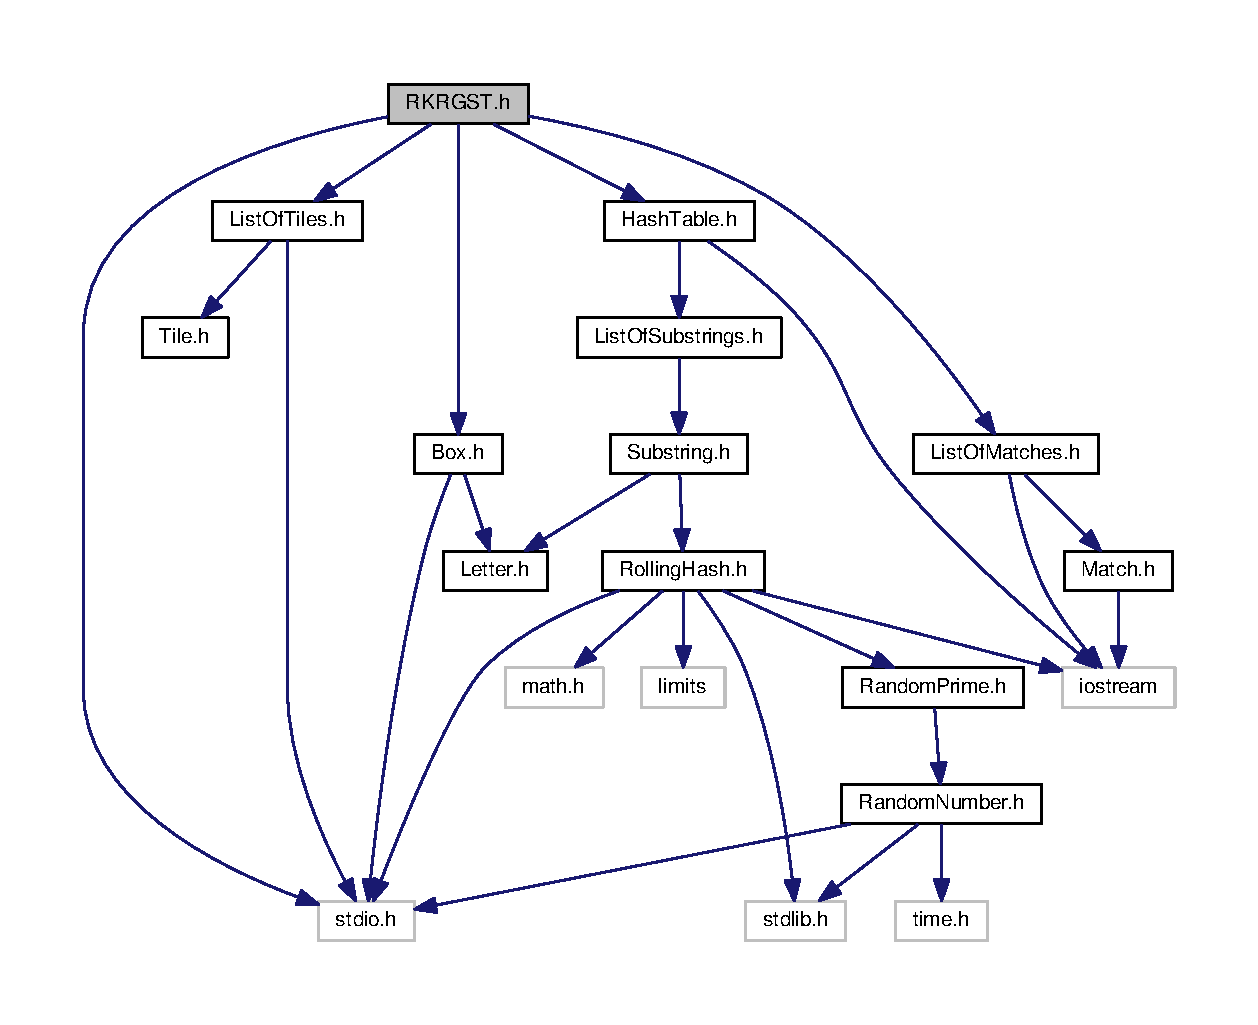
\includegraphics[width=350pt]{RKRGST_8h__incl}
\end{center}
\end{figure}
This graph shows which files directly or indirectly include this file\+:\nopagebreak
\begin{figure}[H]
\begin{center}
\leavevmode
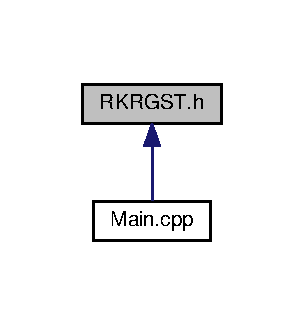
\includegraphics[width=146pt]{RKRGST_8h__dep__incl}
\end{center}
\end{figure}
\subsection*{Classes}
\begin{DoxyCompactItemize}
\item 
class \hyperlink{classRKRGST}{R\+K\+R\+G\+S\+T$<$ Type\+Of\+Content $>$}
\end{DoxyCompactItemize}
\subsection*{Macros}
\begin{DoxyCompactItemize}
\item 
\#define \hyperlink{RKRGST_8h_a7a9a231e30b47bc0345749c8bd1e5077}{M\+A\+X\+\_\+\+L\+E\+N\+G\+T\+H}~20
\end{DoxyCompactItemize}


\subsection{Macro Definition Documentation}
\hypertarget{RKRGST_8h_a7a9a231e30b47bc0345749c8bd1e5077}{\index{R\+K\+R\+G\+S\+T.\+h@{R\+K\+R\+G\+S\+T.\+h}!M\+A\+X\+\_\+\+L\+E\+N\+G\+T\+H@{M\+A\+X\+\_\+\+L\+E\+N\+G\+T\+H}}
\index{M\+A\+X\+\_\+\+L\+E\+N\+G\+T\+H@{M\+A\+X\+\_\+\+L\+E\+N\+G\+T\+H}!R\+K\+R\+G\+S\+T.\+h@{R\+K\+R\+G\+S\+T.\+h}}
\subsubsection[{M\+A\+X\+\_\+\+L\+E\+N\+G\+T\+H}]{\setlength{\rightskip}{0pt plus 5cm}\#define M\+A\+X\+\_\+\+L\+E\+N\+G\+T\+H~20}}\label{RKRGST_8h_a7a9a231e30b47bc0345749c8bd1e5077}


Definition at line 38 of file R\+K\+R\+G\+S\+T.\+h.



Referenced by R\+K\+R\+G\+S\+T$<$ Type\+Of\+Content $>$\+::execute(), and R\+K\+R\+G\+S\+T$<$ Type\+Of\+Content $>$\+::scan\+Pattern().


\hypertarget{RollingHash_8h}{\section{Rolling\+Hash.\+h File Reference}
\label{RollingHash_8h}\index{Rolling\+Hash.\+h@{Rolling\+Hash.\+h}}
}
{\ttfamily \#include $<$math.\+h$>$}\\*
{\ttfamily \#include $<$limits$>$}\\*
{\ttfamily \#include $<$stdlib.\+h$>$}\\*
{\ttfamily \#include \char`\"{}Random\+Prime.\+h\char`\"{}}\\*
{\ttfamily \#include $<$stdio.\+h$>$}\\*
{\ttfamily \#include $<$iostream$>$}\\*
Include dependency graph for Rolling\+Hash.\+h\+:\nopagebreak
\begin{figure}[H]
\begin{center}
\leavevmode
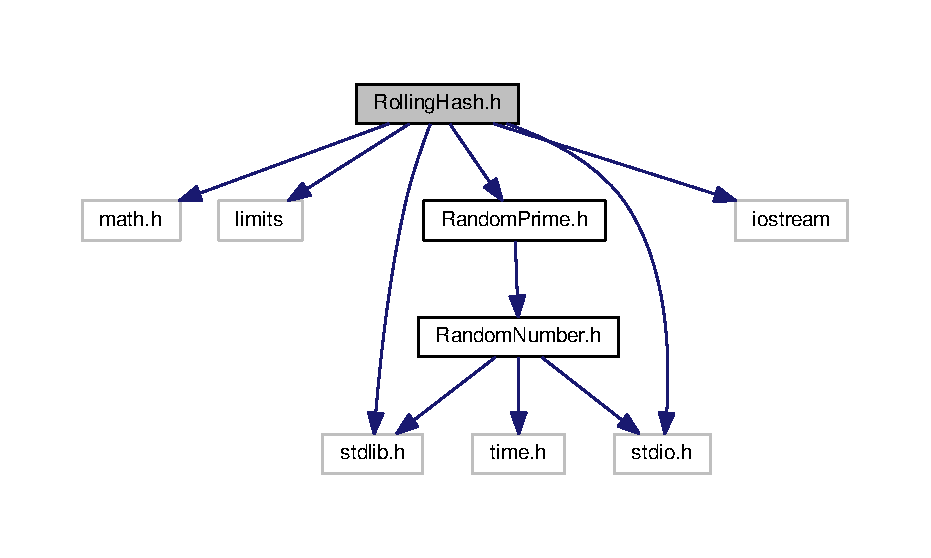
\includegraphics[width=350pt]{RollingHash_8h__incl}
\end{center}
\end{figure}
This graph shows which files directly or indirectly include this file\+:\nopagebreak
\begin{figure}[H]
\begin{center}
\leavevmode
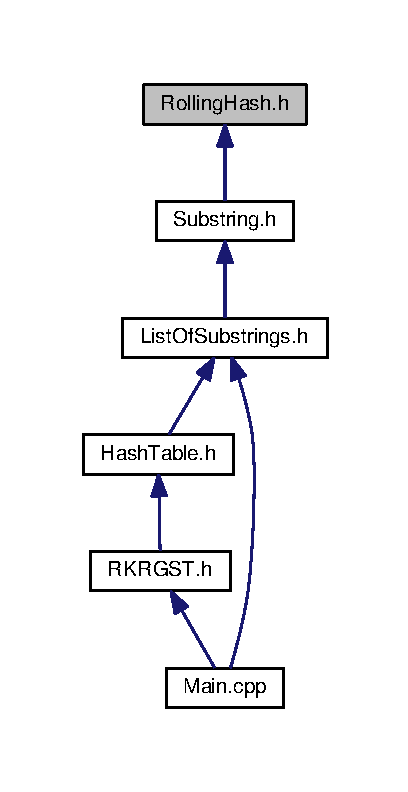
\includegraphics[width=196pt]{RollingHash_8h__dep__incl}
\end{center}
\end{figure}
\subsection*{Classes}
\begin{DoxyCompactItemize}
\item 
class \hyperlink{classRollingHash}{Rolling\+Hash$<$ Type\+Of\+Content $>$}
\end{DoxyCompactItemize}

\hypertarget{Substring_8h}{\section{Substring.\+h File Reference}
\label{Substring_8h}\index{Substring.\+h@{Substring.\+h}}
}
{\ttfamily \#include \char`\"{}Letter.\+h\char`\"{}}\\*
{\ttfamily \#include \char`\"{}Rolling\+Hash.\+h\char`\"{}}\\*
Include dependency graph for Substring.\+h\+:\nopagebreak
\begin{figure}[H]
\begin{center}
\leavevmode
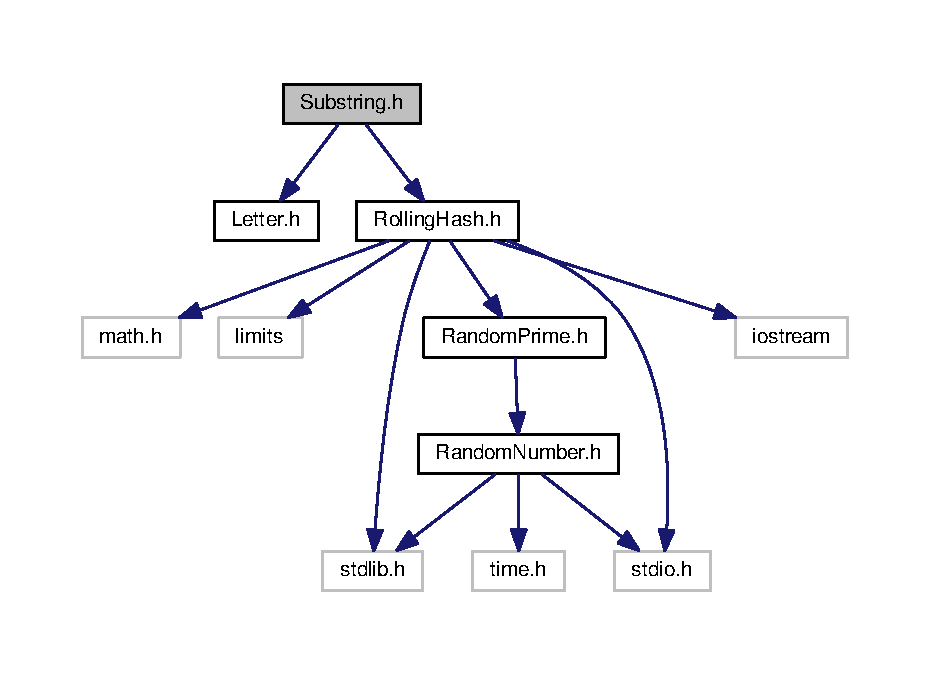
\includegraphics[width=350pt]{Substring_8h__incl}
\end{center}
\end{figure}
This graph shows which files directly or indirectly include this file\+:\nopagebreak
\begin{figure}[H]
\begin{center}
\leavevmode
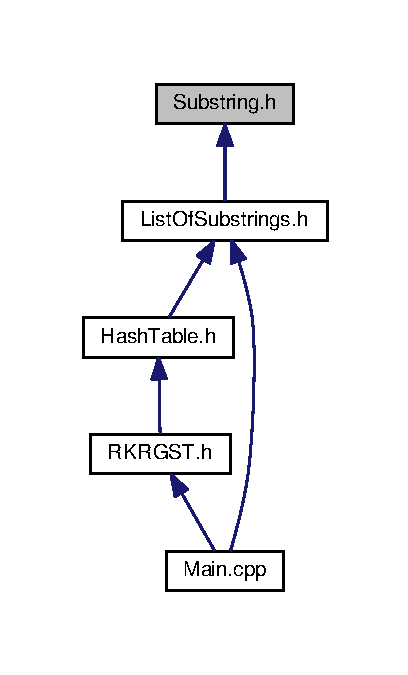
\includegraphics[width=196pt]{Substring_8h__dep__incl}
\end{center}
\end{figure}
\subsection*{Classes}
\begin{DoxyCompactItemize}
\item 
class \hyperlink{classSubstring}{Substring$<$ Type\+Of\+Content $>$}
\end{DoxyCompactItemize}

\hypertarget{Tile_8h}{\section{Tile.\+h File Reference}
\label{Tile_8h}\index{Tile.\+h@{Tile.\+h}}
}
This graph shows which files directly or indirectly include this file\+:\nopagebreak
\begin{figure}[H]
\begin{center}
\leavevmode
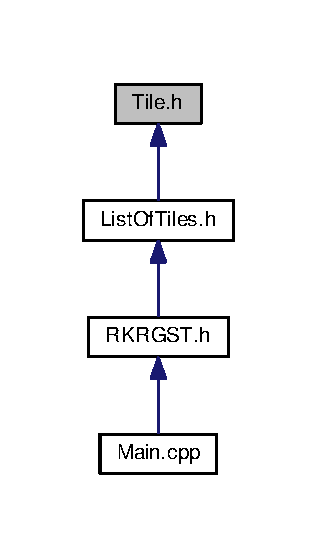
\includegraphics[width=152pt]{Tile_8h__dep__incl}
\end{center}
\end{figure}
\subsection*{Classes}
\begin{DoxyCompactItemize}
\item 
class \hyperlink{classTile}{Tile}
\end{DoxyCompactItemize}

%--- End generated contents ---

% Index
\newpage
\phantomsection
\addcontentsline{toc}{chapter}{Index}
\printindex

\end{document}
